\documentclass[11pt]{article}


\usepackage{amssymb, amsmath, verbatim, amsthm,url, multirow,fullpage,mathtools}
\usepackage{longtable, rotating,makecell,array}
\usepackage[aligntableaux=top]{ytableau}


\setlength{\parindent}{0pt}
\setlength{\parskip}{1.5ex plus 0.5ex minus 0.2ex}


%***************************
%Frontmatter Table of contents
%***************************
% Annotations
%xypic packages
%WLD tkx program
%Useful numeric rings and fields
%Other useful mathematical operations and functions
%Equation display shortcuts
%Shortcuts for frequently used special characters
%Theorem environments
%***************************

%*****************
% Annotations
\usepackage{soul}
\usepackage[colorinlistoftodos,textsize=footnotesize]{todonotes}
\newcommand{\hlfix}[2]{\texthl{#1}\todo{#2}}
\newcommand{\hlnew}[2]{\texthl{#1}\todo[color=green!40]{#2}}
\newcommand{\sanote}{\todo[color=violet!30]}
\newcommand{\note}{\todo[color=green!40]}
\newcommand{\newstart}{\note{The inserted text starts here}}
\newcommand{\newfinish}{\note{The inserted text finishes here}}
\setstcolor{red}
%***************************


%*****************
%xypic packages
\usepackage[all]{xy}
\xyoption{poly}
\xyoption{arc}
%*****************

%*****************
%%% WLD drawing and 2,6 shortcuts

\usetikzlibrary{decorations.pathmorphing,calc}
\usetikzlibrary{intersections}


\definecolor{light-gray}{gray}{0.6}


\tikzstyle{propagator}=[decorate,decoration={snake,amplitude=0.8mm}]
\tikzstyle{smallpropagator}=[decorate,decoration={snake,segment length=3mm,amplitude=0.5mm}]

% these two for drawing partial propagators
\tikzstyle{firstdash}=[dashed,line cap=round, dash pattern=on 2pt off 1pt]
\tikzstyle{seconddash}=[dashed,line cap=round, dash pattern=on 0.5pt off 1pt]

% vertices, radius
\newcommand{\drawWLD}[2]{

\pgfmathsetmacro{\n}{#1}
\pgfmathsetmacro{\radius}{#2}
\pgfmathsetmacro{\angle}{360/\n}
\draw (0,0) circle (\radius);
    \foreach \i in {1,2,...,\n} {
      \draw (\angle*\i:\radius) node {$\bullet$};
       %\pgfmathsetmacro{\x}{\angle*\i}
       %\draw[-,shorten >=-\radius*0.1 cm,shorten <=-\radius*0.1 cm]  (\x:\radius cm)-- (\x + \angle: \radius cm);
    }

}

\newcommand{\drawpolypart}[2]{
\pgfmathsetmacro{\n}{#1}
\pgfmathsetmacro{\radius}{#2}
\pgfmathsetmacro{\angle}{360/\n}
    \foreach \i in {1,2,...,\n} {
      \draw (\angle*\i+ \angle/2:\radius) node {$\bullet$};
     \pgfmathsetmacro{\x}{\angle*\i - \angle/2}
      \pgfmathsetmacro{\concave}{((\n-1.5)/\n)}
      \draw (\x:\radius cm) .. controls (\angle *\i: \concave* \radius cm) .. (\x + \angle:\radius cm);
      %\draw (\angle *\i: .8* \radius cm) node {$\bullet$};
    }

}


% r, bumpr, s, bumps: r, s are start/end vertices, bumpr and bumps are how many steps to bump the start/end for multiple props on one edge
\newcommand{\drawprop}[4]{
\pgfmathsetmacro{\r}{#1}
\pgfmathsetmacro{\bumpr}{#2}
\pgfmathsetmacro{\s}{#3}
\pgfmathsetmacro{\bumps}{#4}
\pgfmathsetmacro{\perturbe}{\angle/\n}

\begin{scope}
%\clip (\angle*\r:\radius) -- (\angle + \angle*\r:\radius) -- (\angle*\s:\radius) -- (\angle + \angle*\s:\radius) -- (\angle*\r:\radius);
\draw[propagator] (\angle*\r + \angle/2 + \bumpr*\perturbe:\radius) -- (\angle*\s + \angle/2 + \bumps*\perturbe:\radius);
\end{scope}
}

\newcommand{\drawlabeledprop}[5]{
\pgfmathsetmacro{\r}{#1}
\pgfmathsetmacro{\bumpr}{#2}
\pgfmathsetmacro{\s}{#3}
\pgfmathsetmacro{\bumps}{#4}
\pgfmathsetmacro{\perturbe}{\angle/\n}

\begin{scope}
%\clip (\angle*\r:\radius) -- (\angle + \angle*\r:\radius) -- (\angle*\s:\radius) -- (\angle + \angle*\s:\radius) -- (\angle*\r:\radius);
\draw[propagator] (\angle*\r + \angle/2 + \bumpr*\perturbe:\radius) -- (\angle*\s + \angle/2 + \bumps*\perturbe:\radius) node[midway, below] {#5};
\end{scope}
}


\newcommand{\drawchord}[2]{
\pgfmathsetmacro{\r}{#1}
\pgfmathsetmacro{\s}{#2}

\begin{scope}
%\clip (\angle*\r:\radius) -- (\angle + \angle*\r:\radius) -- (\angle*\s:\radius) -- (\angle + \angle*\s:\radius) -- (\angle*\r:\radius);
\draw (\angle*\r + \angle/2:\radius) -- (\angle*\s + \angle/2:\radius);
\end{scope}
}


% for anything that requires modifying the propagator, e.g. colour, different amplitude,etc
% 5th argument should be {propagator,<other stuff>} or {smallpropagator,<otherstuff>} otherwise you'll get a straight line
\newcommand{\modifiedprop}[5]{
\pgfmathsetmacro{\r}{#1}
\pgfmathsetmacro{\bumpr}{#2}
\pgfmathsetmacro{\s}{#3}
\pgfmathsetmacro{\bumps}{#4}
\pgfmathsetmacro{\perturbe}{\angle/\n}

\begin{scope}
\clip (\angle*\r:\radius) -- (\angle + \angle*\r:\radius) -- (\angle*\s:\radius) -- (\angle + \angle*\s:\radius) -- (\angle*\r:\radius);
\draw[#5] (\angle*\r + \angle/2 + \bumpr*\perturbe:\radius) -- (\angle*\s + \angle/2 + \bumps*\perturbe:\radius);
\end{scope}
}


\newcommand{\boundaryprop}[4]{
\pgfmathsetmacro{\r}{#1}
\pgfmathsetmacro{\bumpr}{#2}
\pgfmathsetmacro{\s}{#3}
\pgfmathsetmacro{\perturbe}{\angle/\n}

\begin{scope}
\clip (\angle*\r:\radius) -- (\angle + \angle*\r:\radius) -- (\angle*\s - \angle:\radius) -- (\angle*\s:\radius) -- (\angle + \angle*\s:\radius) -- (\angle*\r:\radius);
\draw[#4] (\angle*\r + \angle/2 + \bumpr*\perturbe:\radius) -- (\angle*\s:\radius);
\end{scope}
	
}

\newcommand{\drawnumbers}{
  \foreach \i in {1,2,...,\n} {
  \pgfmathsetmacro{\x}{\angle*\i}
  \draw (\x:\radius*1.15) node {\footnotesize \i};
}
}

\newcommand{\drawnumbersshift}{
  \foreach \i in {1,2,...,\n} {
  \pgfmathsetmacro{\x}{\angle*\i + \angle/2}
  \draw (\x:\radius*1.15) node {\footnotesize \i};
}
}



\newcommand{\boundA}[3]{
	\pgfmathsetmacro{\r}{#1}
	\pgfmathsetmacro{\bumpr}{#2}
	\pgfmathsetmacro{\destination}{#3}
	\pgfmathsetmacro{\perturbe}{\angle/\n}
	\path [name path=polyedge1] (\angle*\r:\radius) -- (\angle*\r + \angle:\radius);
	\path [name path=radius1] (0:0) -- (\angle*\r + \angle/2 + \bumpr*\perturbe:\radius);
	\draw[->,
	name intersections={of=polyedge1 and radius1,by=p},
	shorten >=\radius*0.1 cm] (p) ++(\angle*\r + \angle/2 + \bumpr*\perturbe:\radius*0.15) -- (\angle*\destination: \radius*1.15);

}



\newcommand{\boundB}[3]{
	\pgfmathsetmacro{\rangle}{#1*\angle + \angle/2 + #2*\angle/\n}
	\pgfmathsetmacro{\sangle}{#1*\angle + \angle/2 + #3*\angle/\n}


	\draw[->,shorten <=\radius*0.02cm,shorten >=\radius*0.05cm] (\rangle:\radius*1.05) -- (\sangle:\radius*1.05);

}

\newcommand{\makediag}[8]{
	\begin{tikzpicture}[rotate=60,baseline=(current bounding box.east)]
	\begin{scope}
	\drawWLD{6}{0.8}
	%\drawnumbers
	\drawprop{#1}{#2}{#3}{#4}
	\drawprop{#5}{#6}{#7}{#8}
	\end{scope}
	\end{tikzpicture}
}



%*****************

%*****************
%Useful numeric rings and fields
\newcommand{\Q}{\mathbb{Q}}
\newcommand{\Z}{\mathbb{Z}}
\newcommand{\C}{\mathbb{C}}
\newcommand{\R}{\mathbb{R}}
\newcommand{\N}{\mathbb{N}}
\newcommand{\RP}{\mathbb{R}\mathbb{P}}
\newcommand{\id}{\mathbb{I}}
\newcommand{\Gr}{\mathbb{G}_{\R, \geq 0}}
\newcommand{\Grtnn}{\mathbb{G}_{\R, +}}
\newcommand{\CW}{\overline{\mathcal{W}}} % CW complex of W(k,n)
\newcommand{\BW}{\widehat{\mathcal{W}}} % complex minus bald spots
%*****************


%*****************
%Other useful mathematical operations and functions
\newcommand{\D}{\partial}
\newcommand{\rk}{\textrm{rk }}
\newcommand{\spn}{\textrm{span }}
\newcommand{\rd}{\textrm{d}}
\newcommand{\Res}{\textrm{Res}}
%*****************


%*****************
%Equation display shortcuts
\def\ba #1\ea{\begin{align} #1 \end{align}}
\def\bas #1\eas{\begin{align*} #1 \end{align*}}
\def\bml #1\eml{\begin{multline} #1 \end{multline}}
\def\bmls #1\emls{\begin{multline*} #1 \end{multline*}}
%*****************


%*****************
%Shortcuts for frequently used special characters
\newcommand{\fB}{\mathfrak{B}}
\newcommand{\cP}{\mathcal{P}}
\newcommand{\fZ}{\mathfrak{Z}}
\newcommand{\cM}{\mathcal{M}}
\newcommand{\cA}{\mathcal{A}}
\newcommand{\cI}{\mathcal{I}}
\newcommand{\cC}{\mathcal{C}}
\newcommand{\cB}{\mathcal{B}}
\newcommand{\G}{\mathbb{G}}
\newcommand{\Prop}{\textrm{Prop}}
\newcommand{\cW}{\mathcal{W}}
\newcommand{\bM}{\mathbb{M}}
\newcommand{\cZ}{\mathcal{Z}}
\newcommand{\cY}{\mathcal{Y}}
\newcommand{\Dom}{\textrm{Dom}}
\newcommand{\detzr}[1] {\langle (\cZ_*^\mu|V(p))^{#1} \rangle}
\newcommand{\II}{\mathcal{I}}
\newcommand{\PP}{\mathcal{P}}
\newcommand{\BB}{\mathcal{B}}
\newcommand{\CS}{\mathcal{S}}
\newcommand{\interval}[2]{[\![#1,#2]\!]}
\newcommand{\gale}[1]{\preccurlyeq_{#1}}
\newcommand{\sgale}[1]{\prec_{#1}}
\renewcommand\vec[1]{\overrightarrow{#1}}
\newcommand\cev[1]{\overleftarrow{#1}}
%*****************

%*****************
%Theorem environments
\newtheorem{thm}{Theorem}[section]
\newtheorem{conj}[thm]{Conjecture}
\newtheorem{lem}[thm]{Lemma}
\newtheorem{cor}[thm]{Corollary}
\newtheorem{prop}[thm]{Proposition}
\newtheorem{algorithm}[thm]{Algorithm}


\theoremstyle{remark}
\newtheorem{eg}[thm]{Example}
\newtheorem{claim}[thm]{Claim}

\theoremstyle{definition}
\newtheorem{dfn}[thm]{Definition}
\newtheorem{rmk}[thm]{Remark}
\newtheorem{ntn}[thm]{Notation}
%*****************





\title{Combinatorics of the geometry of Wilson loop diagrams}
\author{Susama Agarwala, Si\^an Fryer, and Karen Yeats}
%\date{}

\begin{document}
\maketitle

This paper studies the combinatorics of Wilson Loop Diagrams.
\section{Wilson Loop diagrams}\label{section background}

What are Wilson loop diagrams and their integrals.

\begin{dfn}\label{WLdfn}
A Wilson loop diagram is given by the following data: a cyclicly ordered set $V$, along with a choice of first vertex (labeled $1$), and $k$ pairs, called propagators, written $\{p_r = (i_r, j_r)\}_{r=1}^k$.  \end{dfn}

Generally speaking, the propagators are undirected, so $p = (i,j) = (j,i)$. In order to fix a convention, we write $p = (i,j)$ with  $i +1 < j$ relative to the first vertex. However, at times (section \ref{sec:propagator configs}), we consider directed propagators, where $p= (i,j)$ denotes a particular propagator flowing in one direction, while $p= (j,i)$ denotes the \emph{same} propagators flowing in the opposite direction. \sanote{Addendum 1}

We depict this data as a circle with marked points, called vertices. The vertices are labeled by $V$ (preserving the cyclic ordering). The arc between consecutive vertices are called edges. There are $k$ wavy lines in the interior of the diagram, depicting the proagators, with endpoints on the edges. A propagator, $p =(i,j)$ has one endpoint on the edge between the vertex labeled $i$ and $i+1$ and another endpoint on the edge defined by $j$ and $j+1$. The condition on $i_r$ and $j_r$ means that the propagator does not go between adjacent edges. Let $\cP = \{p_r\}_{r=1}^k$ be the set of propagators. Then we write \bas W = (\cP, V) \;.\eas

Note that the marked circle gives the vertices of $W$ a cyclic ordering. The choice of first vertex gives it a compatible linear order. Both the cyclic and the linear order become the correct perspective at various points in this paper. 

Often we take $V$ to be $[n]$, the cyclically ordered set of integers, $1 \ldots n$. In this case, we write $W = (\cP, [n])$. We introduce some notation to speak of vertices supporting a propagator, and the set of propagators supported on a vertex set.

\begin{dfn} \label{VPropdfn}
Let $W = (\cP, [n])$.
\begin{enumerate}
\item For $p \in \cP$, let $V(p) = \{i_p, i_p+1, j_p, j_p+1\}$ be the set of vertices supporting $p$. Then, for $P \subseteq \cP$, the set $V(P) = \cup_{p \in P} V(p)$ is the vertex support of $P$.
\item For $V \subseteq [n]$, write $\Prop(V) = \{ p \in \cP | V(p) \cap V \neq \emptyset \} $.
\item For $P \subseteq \cP$, define $F(P) = V(P^c)^c$ to be the set of vertices in $[n]$ that do not support any propagators outside the set $P$.
\item The set of vertices that are not in the support of any propagotors is denoted  $F(\emptyset)$. Vertices in this set are called non-supporting.  
\end{enumerate}
\end{dfn}

\begin{rmk}\label{alt F(P) rmk}
Note that a more explicit definition of $F(P)$ is \bas F(P)  = \big(V(P) \setminus V(P^c) \big) \cup F(\emptyset) \;.\eas Furthermore, note that by construction $\Prop(F(P)) \subseteq P$.  
\end{rmk}

It is sometimes useful to discuss propagators in terms of the edges supporting them, rather than the vertices.

\begin{dfn}
The $i^{th}$ edge of $W$ is the edge of the external polygon that lies between the vertices $i$ and $i+1$.
\end{dfn}

In this manner, the propagator $p = (i, j)$ is supported by the $i^{th}$ and $j^{th}$ edges.

\begin{dfn}\label{admisdfn}
A Wilson loop diagram is admissible if \begin{enumerate}
\item $|V| \geq |\cP| + 4$
\item There does not exists a set of propagators, $P \subseteq \cP$ such that $|V(P)| < |P| + 3$.
\item There does not exist a pair of propagators, $p, q \subseteq \cP$ such that $i_p < i_q < j_p <j_q$.
\end{enumerate}
A Wilson loop diagram is weakly admissible if the second and third conditions hold.
 \end{dfn}

The first conditions states that there are at least four more vertices than propagators in an admissible Wilson Loop Diagram. The second imposes an upper bound on how densely the propagators can be fitted in the diagram. The third ensures that ensures that no propagators cross in the interior of the diagram. In other words, a Wilson loop diagram, $(\cP, [n])$ is admissible if and only if $n > \cP +4$, and has neither crossing propagators nor any pairs of propagators that start and end on the same pair of non-adjacent edges.

Note that if we take any admissible Wilson loop diagram and remove the unsupported vertices then we will obtain a weakly admissible Wilson loop diagram that may or may not be admissible itself.

In what follows, we will talk about admissible Wilson Loop diagrams and subdiagrams thereof.

\begin{dfn} \label{subdiagramdfn}
Let $W = (\cP, [n])$ be an admissible Wilson loop diagram. The weakly admissible diagram, $W'$ is a subdiagram of $W$, written $W' \subseteq W$, if \bas W' = (P, V); \quad P \subseteq \cP ; \quad V(P) \subseteq V \subseteq [n]\;.\eas
\end{dfn}

There is one particular type subdiagram that deserves special attention.

\begin{dfn}
For $W$ an admissible diagram, $(P, V(P))$ is exact if $|V(P)| = |P| + 3$.
\end{dfn}

The exact subdiagrams define an equivalence relation amongst Wilson loop diagrams.

\begin{dfn}\label{equivdfn} 
There is an equivalence relationship on the set of admissible Wilson loops diagrams given by the transititve closure the following binary relation: $W = (\cP, [n]) \sim W'= (\cP', n)$ if
\begin{enumerate}
\item There exist two different exact subdiagrams, $(P, V(P))$ and $(P', V(P'))$ of $W$ and $W'$ respectively such that $V(P) =  V(P')$.
\item The complementary subdiagrams are identical: $(\cP \setminus P, V(P)^c) = (\cP' \setminus P', V(P')^c)$.
\end{enumerate}
\end{dfn}

\begin{eg} \label{eg:equivdiags}
Note that since this is an equivalence relation, we may find that two Wilson loop diagrams are equivalent, even if they do not have complements of (non-trivial) exact subdiagrams in common. Consider the following three Wilson loop diagrams,
\bas
W_1 = 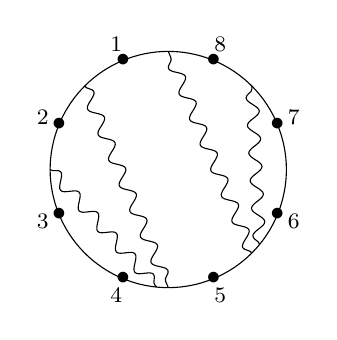
\begin{tikzpicture}[rotate=67.5,baseline=(current bounding box.east)]
	\begin{scope}
	\drawWLD{8}{1.5}
	\drawnumbers
	\drawprop{1}{0}{4}{0}
	\drawprop{2}{0}{4}{-1}
    \drawprop{5}{0}{8}{0}
    \drawprop{5}{1}{7}{0}
		\end{scope}
	\end{tikzpicture} \quad
W_2 = 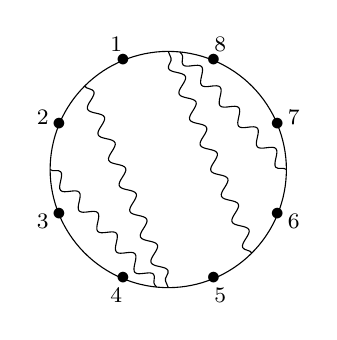
\begin{tikzpicture}[rotate=67.5,baseline=(current bounding box.east)]
	\begin{scope}
	\drawWLD{8}{1.5}
	\drawnumbers
	\drawprop{1}{0}{4}{0}
	\drawprop{2}{0}{4}{-1}
    \drawprop{5}{0}{8}{0}
    \drawprop{6}{0}{8}{-1}
		\end{scope}
	\end{tikzpicture} \quad
W_3 = 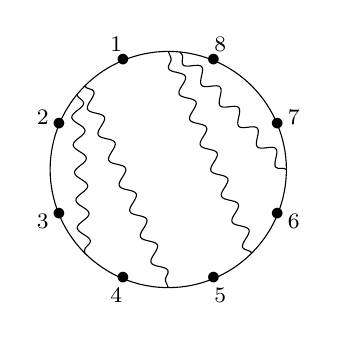
\begin{tikzpicture}[rotate=67.5,baseline=(current bounding box.east)]
	\begin{scope}
	\drawWLD{8}{1.5}
	\drawnumbers
	\drawprop{1}{0}{4}{0}
	\drawprop{1}{1}{3}{0}
    \drawprop{5}{0}{8}{0}
    \drawprop{6}{0}{8}{-1}
		\end{scope}
	\end{tikzpicture} .
\eas


The diagrams $W_1 \sim W_2$ because $(\{(5,8), (5,7)\}, \{5,6,7,8,1\})$ and $(\{(5,8), (7,8)\}, \{5,6,7,8,1\})$ are the corresponding differing subdiagrams. Furthermore, there is the equivalence $W_2 \sim W_3$ due to the exact subdiagrams $(\{(1,4), (3,4)\}, \{1,2,3,4,5\})$ and $(\{(1,4), (1,3)\}, \{1,2,3,4,5\})$. This forces an equivalence between $W_1$ and $W_3$, even though one cannot partition the propagators of each into a an exact subdiagram (that may vary between the diagrams) and a complement that is fixed.  \end{eg}

Each Wilson loop diagram, $W = (\cP, [n])$ with $|\cP| = k$ is associated to a $k \times n$ matrix with non-zero real variable entries, called $C(W)$:

\ba C(W)_{p,q} = \begin{cases} c_{p,q} & \textrm{ if } q \in V(p) \\
0  & \textrm{ if } q \not \in V(p)  \end{cases}
\;. \label{C(W) dfn}\ea

\begin{eg}
For example, ordering the propagators of $W_1$ from Example \ref{eg:equivdiags}: \bas (1,4), \, (2,4), \, (5,7), \, (5,8) \eas we may write
\bas C(W_1) = \left(
\begin{array}{cccccccc}
c_{1,1} & c_{1,2} & 0 & c_{1,4} & c_{1,5} & 0 & 0 & 0 \\
0 & c_{2,2} & c_{2,3} & c_{2,4} & c_{2,5} & 0 & 0 & 0 \\
0 & 0 & 0 & 0 & c_{3,5} & c_{3,6} & c_{3,7} & c_{3,8} \\
c_{4,1} & 0 & 0 & 0 & c_{4,5} & c_{4,6} & 0 & c_{4,8}  \\
\end{array}
\right) \;.\eas

\end{eg}

These $C(W)$ parametrize a subspace of $\Gr(k, n)$ as shown in \cite{wilsonloops}, call it $\Sigma(W)$. The Wilson loop diagrams also define a volume form on $\Sigma(W)$: \bas \Omega(W) = \frac{\prod_{r=1}^{|\cP|} \prod_{v \in V_{p_r}} \textrm{d}c_{p_r}}{R(W)} \;. \eas The denominator $R(W)$ is a polynomial defined by $2 \times 2$ and $1 \times 1$ minors of $C(W)$ as defined below.

\begin{dfn}\label{def R(W)}
For $W = (\cP, [n])$, $R(W) = \prod_{e=1}^n R_e$, with $R_e$ defined by the propagators ending on it. For any edge $e$ of $W$, order the propagators incident on $e$ as $\{p_1 \ldots p_r\}$, ordered such that $p_1$ is closest to the vertex $e$, $p_r$ closest to $e+1$, and $p_i$ is closer to $e$ than $p_{i+1}$. Then \bas R_e =  c_{p_1,e+1} \prod_{j= 1}^{r-1} \left((c_{p_j,e} c_{p_{j+1},e+1} - c_{p_{j+1},e} c_{p_{j},e+1} ) \right) c_{p_s,e}\;.\eas Note that in this notation, if $r = 1$, $R_e = c_{p,e} c_{p,e+1}$.
\end{dfn}


\section{Equivalence classes of Wilson loop diagrams}

In \cite{wilsonloop}, Agarwala and Amat show that Wilson loop diagrams can be interpreted as positroids, a certain well behaved class of realizable matroids (this correspondence is stated precisely in Theorem \ref{thm WLD defines matroid} below). This opens up the study of Wilson loop diagrams to techniques from geometry and combinatorics. In particular we examine the partial result shown in \cite{wilsonloop}, that shows that equivalent Wilson Loop Diagrams define the same matroid. In section 2.4, we make the relationship between Wilson Loop diagrams and matroids explicit. We count the size of each equivalence class, and enumerate the {\color{violet} the number of said classes}. We also show that two Wilson Loop diagrams map to the same matroid if and only if they are equivalent. 

In subsection \ref{sec matroid background}, we discuss a few matroidal facts about Wilson loop diagrams. In section \ref{sec: polygon partitions}, we show that there is a one to one correspondence between exact subdiagrams of Wilson loop diagrams and triangulated pieces of the corresponding polygon partion. In section \ref{sec: exact diagram matroidal props}, we prove some matroidal properties of exact subdiagrams. We show that a subdiagram of $W$ defines a uniform matroid if and only if the subdiagram is exact (Theorem \ref{exactuniformthm}). Furthermore, this uniform matroid is the restriction of the dual matriod of $W$ restricted to the exact subdiagram (Remark \ref{remark exact dual restiction}). The main result of section \ref{sec: matroids and equivalence} shows that that two admissible Wilson loop diagrams define the same matroid if and only if they are equivalent (Theorem \ref{same matroid iff equiv}). We obtain a formula for the number of admissible Wilson loop diagrams in each equivalence class (Corollary \ref{number of equiv diagrams}) {\color{violet}as well as the number of equivalence classes}. In this way, we give a comple characterization of the relationship between Wilson Loop diagrams and their associated matroids. 



\subsection{Wilson loop diagrams as matroids\label{sec matroid background}}

We first give a quick summary of the matroid terminology that we will need; it is not intended as a comprehensive introduction to matroids and the interested reader is referred to [ref][find a good matroid reference].

A {\em matroid} $M = (E,\cB)$ consists of a finite ground set $E$ and a non-empty family $\cB \subseteq \cP(E)$ whose elements satisfy the {\em basis exchange property}: for any distinct $B_1,B_2 \in \cB$ and any $a \in B_1 \setminus B_2$, there exists some $b \in B_2 \setminus B_1$ such that $(B_1 \setminus \{a\})\cup \{b\} \in \cB$ as well. The elements of $\cB$ are called the {\em bases} of the matroid. Note that the basis exchange property immediately implies that all bases have the same size.

A subset $A \subseteq E$ is called {\em independent} in $M$ if $A \subseteq B$ for some $B \in \cB$, and {\em dependent} else. The {\em rank}  $\rk(A)$ of a subset $A \subseteq E$ is the size of the largest independent set contained in $A$. The rank of the matroid itself is defined to be $\rk(E)$.

A {\em circuit} in $M$ is a minimally dependent set. That is, it is a set $C \subseteq E$ such that $C$ is dependent but $C \setminus \{e\}$ is independent for any $e \in C$. A union of circuits is called a {\em cycle}. On the other hand, a {\em flat} is a maximally dependent set, i.e. a set $F \subseteq E$ such that $\rk(F \cup \{e\}) = \rk(F) + 1$ for any $e \in E \setminus F$. Unsurprisingly, a {\em cyclic flat} is a set which is both a flat and a cycle. The set of circuits in a matroid uniquely defines that matroid, as does the set of flats; thus one could specify a matroid by listing its independent sets, bases, circuits, or flats. [ref]

Finally, we describe several important types of matroids. A matroid of rank $k$ with a ground set of size $n$ is called {\em realizable} if there exists some $A \in Gr(k,n)$ whose non-zero $k\times k$ minors are exactly those with columns indexed by elements of $\cB$. A {\em positroid} is a matroid which can be realized by an element of the totally nonnegative Grassmannian $\Gr(k,n)$. Finally, a {\em uniform matroid} of rank $r$ is a matroid in which any set of size $\leq r$ is independent.


Matroid theory relates to the study of Wilson loop diagrams as follows. In \cite{wilsonloop}, Agarwala and Amat show that every admissible Wilson loop diagram with $k$ propagators defines a positroid of rank $k$, and that the independent sets can be read directly from the diagram:

\begin{thm} \label{thm WLD defines matroid} \cite[Theorem 3.6]{wilsonloop} Any admissible Wilson loop diagram $W =(\cP, [n])$ defines a matroid $M(W)$ with ground set $[n]$. The independent sets are exactly those subsets $V \subseteq [n]$ such that $\nexists U\subseteq V$ satisfying $|\Prop(U)| < |U|$. \label{thm:WLDmatroid}\end{thm}
In other words, the independent sets of $M(W)$ correspond to the sets of vertices in $W$ such that no subset supports fewer propagators than the vertices it contains.

Throughout, we take the {\em matroid defined by $W$} to be the matroid $M(W)$ of Theorem \ref{thm WLD defines matroid}. Note that since vertices of the diagram $W$ correspond to columns of the associated matrix $C(W)$, $M(W)$ can also be thought of as the matroid realized by $C(W)$. 


% The identification of Theorem \ref{thm WLD defines matroid} is not 1-1: by \cite[Theorem 1.18]{wilsonloop}, if two admissible Wilson loop diagrams are equivalent (as in Definition~\ref{equivdfn}) then they define the same matroid. 


Let $W = (\cP,n)$ be an admissible Wilson loop diagram, and $M(W)$ its associated matroid. Where it will not cause confusion we conflate the two objects, identifying vertices of $W$ with elements of the ground set $[n]$ in $M(W)$. 

In particular, this allows us to prove results about $M(W)$ by considering the behavior of propagators in $W$. We record a few elementary facts about the rank and cycles of $M(W)$ here as an example of this.

\begin{lem}\label{lem facts about WLD matroids}
Let $W = (\cP,n)$ be an admissible Wilson loop diagram. Then:
\begin{enumerate}
\item The rank of a set $V \subseteq [n]$ is bounded above by $\min\{|V|,|\Prop(V)|\}$, with $\rk(V) = |V|$ if and only if $V$ is an independent set.
%\item Let $v \in [n]$ and $q \in \Prop(v)$. Then for any $V \subset [n]$ such that $q \not \in \Prop(V)$, we have $\rk(V \cup \{v\}) = \rk(V) +1$, i.e. adding a vertex that supports a new propagator to a set increases the rank of the set.
\item If $C \subseteq [n]$ is a cycle, then $\rk(C) = |Prop(C)|$.
\item If $[n]$ can be partitioned into at least two non-empty sets, each of which support different sets of propagators that form a partition of the propagotor set, \bas [n] = \sqcup_i V(P_i) \quad \textrm{s.t.} \quad \sqcup P_i = \cP; \quad V(P_i) \cap V(P_j) = \emptyset; \quad  P_i \cap P_j = \emptyset \;, \eas then the matroid $M(W)$ is seperable, \bas M(W) = \bigoplus_i M(P_i, V(P_i)) \;.\eas 
\item $F(P)$ is a flat of $M(W)$, thus justifying the name ``propagator flat''.
\end{enumerate}
\end{lem}
\begin{proof}
The first part of (1) is \cite[Equation (9)]{wilsonloop} and surrounding discussion, and the second part is standard matroid theory. (2) is \cite[Lemma 3.27]{wilsonloop}. (3) is a direct consequence of \cite[Lemma 3.20]{wilsonloop} and the fact that $F(P_1)^c = V(P_1^c)$

To prove (4), we need to show that $F(P)$ is maximally dependent. If $F(P) = [n]$ then this is automatic, so suppose not and let $v \in [n] \setminus F(P)$. In other words, $v \in V(P^c)$ and so $v$ supports some propagator $q \not\in P$.  Let $S \subseteq F(P)$ be an independent set of maximal size. Then $\Prop(S) \subseteq P$ by (1), and no subset of $S$ supports fewer propagators than the number of vertices it contains (this is the definition of an independent set in $M(W)$). Since $v$ supports a new propagator $q \not\in P$, the set $S \cup \{v\} \subseteq F(P) \cup\{v\}$ also satisfies this independence condition. Thus $\rk(F(P) \cup\{v\}) = \rk(F(P)) + 1$, as required.
\end{proof}

Note that this means that the set, $F(\emptyset)$, of non-supporting vertices is the maximal subset of vertices of $W$ of rank $0$. That is, it is the unique flat of rank $0$ in $M(W)$. 

\subsection{Polygon partitions of Wilson loop diagrams\label{sec: polygon partitions}}


The equivalence relation on Wilson loop diagrams is defined in terms of exact subdiagrams; thus in order to understand the equivalence, we need a way to extract and compare exact subdiagrams. We do this via the notion of a polygon partition of $W$.

\begin{dfn}
  Let $W = (\cP, [n])$ be an admissible Wilson loop diagram.  The \emph{polygon partition} associated to $W$, denoted $\tau(W)$, is defined as follows.
  \begin{itemize}
  \item The vertices of $\tau(W)$ correspond to the edges of $W$.
  \item Labeling the vertices of $\tau(W)$ with the edge number of $W$gives a cyclic order to the vertices. Connecting consecutive vertices gives a graph theoretic cycle called the polygon of $\tau(W)$.
  \item Each propagator of $W$ defines a chord edge of $\tau(W)$; specifically,  a propagator $(i,j) \in \cP$ defines a chord connecting the vertices $i$ and $j$ in $\tau(W)$.
  \end{itemize}
\end{dfn}

\begin{lem}\label{tausimpleplanarlem}
If $W = (\cP, [n])$ is an admissible Wilson loop diagram, then $\tau(W)$ is a simple planar graph whose outer face is a cycle. It is embedded such that the vertices all lie on this infinite face\footnote{That is, it is an \emph{outerplanar} graph}. These vertices are cyclically ordered, with a choice of first vertex giving it an additional compatible linear order.
\end{lem}

\begin{proof}
Since the vertices of $\tau(W)$ are labeled by the edges of $W$, which are cyclically ordered, this gives an ordering to the vertices and the outer face of $\tau(W)$ is a cycle. Since $W$ is admissible, no pairs of propagators cross. Therefore, it is a planar embedding. Similarly, $W$ does not admit any propagators of the form $p = (i, i+1)$; therefore there is exactly one edge connecting any two adjacent edges of $\tau(W)$. Finally, there does not exist two propagators $p,q$ such that both $p$ and $q$ start at edge $i$ and end at edge $j$. Therefore, no other two vertices of $\tau(W)$ can be connected by more than one edge. Finally, the embedding of $\tau(W)$ is induced from the embedding of the graph $W$.
 \end{proof}

\begin{comment}
\hlfix{For an admissible $W$ no propagators cross and so no chord edges of $\tau(W)$ cross.  Thus, in graph theoretic language, we can view $\tau(W)$ as a planar embedding of a
graph with no cut vertices, where all vertices lie on the infinite face, along with a distinguished start vertex and direction around the infinite face.  From this viewpoint the polygon of $tau(W)$ is the boundary of the infinite face.}{I've smushed this together a bit in the prev. lem. Tell me if I've missed anything. Its a lemma for emphasis, not difficulty}
\end{comment}

\begin{eg}\label{WLDtopolygonpartition}
In this example we return to two of the Wilson loop diagrams in Example \ref{eg:equivdiags}. We can pair diagrams with their polygon partitions as follows:
\bas W_1 = 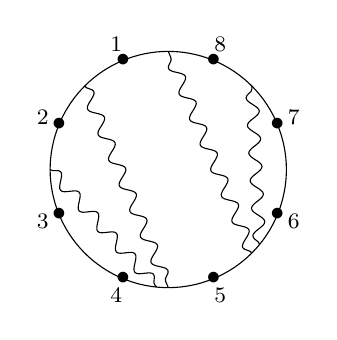
\begin{tikzpicture}[rotate=67.5,baseline=(current bounding box.east)]
	\begin{scope}
	\drawWLD{8}{1.5}
	\drawnumbers
	\drawprop{1}{0}{4}{0}
	\drawprop{2}{0}{4}{-1}
    \drawprop{5}{0}{8}{0}
    \drawprop{5}{1}{7}{0}
		\end{scope}
	\end{tikzpicture} \quad; \quad
\tau(W_1) = 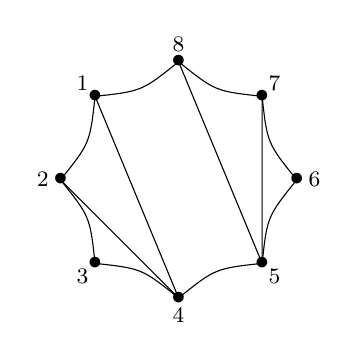
\begin{tikzpicture}[rotate=67.5,baseline=(current bounding box.east)]
	\begin{scope}
	\drawpolypart{8}{1.5}
    \drawnumbersshift
    \drawchord{1}{4}
    \drawchord{2}{4}
    \drawchord{5}{8}
    \drawchord{5}{7}
	\end{scope}
	\end{tikzpicture}
\eas and
\bas W_3 = 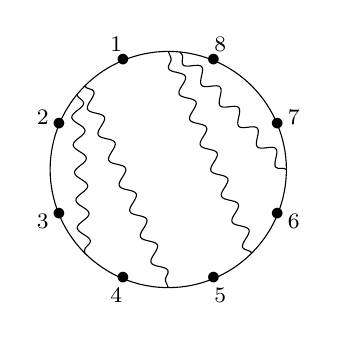
\begin{tikzpicture}[rotate=67.5,baseline=(current bounding box.east)]
	\begin{scope}
	\drawWLD{8}{1.5}
	\drawnumbers
    \drawprop{1}{0}{4}{0}
	\drawprop{1}{1}{3}{0}
    \drawprop{5}{0}{8}{0}
    \drawprop{6}{0}{8}{-1}	
		\end{scope}
	\end{tikzpicture}\quad; \quad
\tau(W_3) = 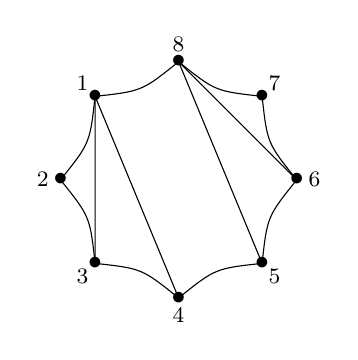
\begin{tikzpicture}[rotate=67.5,baseline=(current bounding box.east)]
	\begin{scope}
	\drawpolypart{8}{1.5}
    \drawnumbersshift
    \drawchord{1}{4}
    \drawchord{1}{3}
    \drawchord{5}{8}
    \drawchord{6}{8}
	\end{scope}
	\end{tikzpicture} .
\eas

\end{eg}

Recall that a planar embedding of a graph is a \emph{triangulation} if all faces, except possibly the infinite face, are triangles.

\begin{dfn}
  Let $W$ be an admissible Wilson loop diagram and $\tau(W)$ its polygon partition. A \emph{triangulated piece} of $\tau(W)$ is a 2-connected subgraph of $\tau(W)$ which is a triangulation. We will take the convention that a subgraph consisting of a single chord edge is called a \emph{trivial} triangulated piece.
A {\em maximal} triangulated piece is one which is not contained in any strictly larger triangulated piece.
\end{dfn}

\begin{dfn}
 A {\em decomposition} of a polygon partition $\tau(W)$ is a set of 2-connected induced subgraphs of $\tau(W)$ which partition the edges of $\tau(W)$.  
\end{dfn}

\begin{eg} \label{eg: unique decomposition} For the Wilson loop diagrams and polygon partitions in Example \ref{WLDtopolygonpartition}, the vertex sets $\{1, 2, 3,4\}$ and $\{5, 6, 7, 8\}$ give maximal triangulated pieces for both $\tau(W_1)$ and $\tau(W_3)$. The vertex set $\{4,5, 8, 1\}$ is not a triangulation in either polygon partition. 
\end{eg}

\begin{lem} \label{decompositionlem}
  For $W$ an admissible Wilson loop diagram, the polygon partition $\tau(W)$ has a unique decomposition into maximal triangulated pieces, and edges in the polygon of $\tau(W)$.
\end{lem}



\begin{proof}
We begin by giving an algorithm for the decomposition, then prove its uniqueness. Let $W = (\cP, [n])$, with $|\cP| = k$.

By \emph{splitting} a vertex $v$ we will mean replacing $v$ by new vertice $v_1, v_2,\ldots, v_{\text{deg}(v)}$ such that each $v_i$ has exactly one neighbour and the union of the of the $v_i$ is the neighbourhood\footnote{The neighbourhood of a vertex is the set of adjacent vertices} of $v$.

Let $T(W)$ be the dual graph of $\tau(W)$ with the vertex corresponding to the infinite face split.
%In other words, place a vertex on each finite face of $\tau(W)$. These vertices are connected if there is a chord edge separating the edges. Furthermore, if the face is bounded by an edge of the polygonal cycle of $\tau(W)$, the corresponding vertex gets a leaf edge for each such boundary.
Since $\tau(W)$ is an embedded graph (with a fixed distinguished embedding) by Lemma \ref{tausimpleplanarlem}, $T(W)$ is an uniquely defined graph.

Furthermore $T(W)$ is a tree because it is connected, has $n+k+1$ vertices ($k+1$ from the internal faces of $\tau(W)$ and $n$ from the outer face) and $n+k$ edges (since $\tau(W)$ has $n+k$ edges).  Additionally, since $\tau(W)$ is simple, $T(W)$ has no vertices of degree $2$.  

%We claim that $T(W)$ is a tree. Since $\tau(W)$ is a planar graph with $k$ chord edges and no internal vertices, there are $k+1$ internal faces of $\tau(W)$. Each of these internal faces corresponds to a vertex of $T(W)$, and there are $n$ vertices of $T(W)$ from the splitting of the dual graph, so $T(W)$ has $n+k+1$ vertices in total. On the other hand, $T(W)$ has $n+k$ edges, corresponding to the $n +k$ edges of $\tau(W)$. Therefore, $T(W)$ is a tree.

Split every vertex of $T(W)$ which has degree $>3$.
%By construction, each face of $\tau(W)$ is a polygon. Therefore, each vertex of $T(W)$ is at least 3 valent (one for each edge of the polygon). \hlfix{If split each vertex of $T(W)$ if it is strictly greater than $3$ valent.}{???} (In other words, we fail to split exactly when the face is a triangle).
The connected components of $T(W)$ correspond to the decomposition of $\tau(W)$ into maximal triangulated pieces and edges originally in the polygon of $\tau(W)$.  Let $f$ be the forest thus obtained.
The vertices of $f$ either have degree 1 or 3.
%, (if they correspond leaf vertices) or 3,  (if they correspond to triangular faces).
Trees of $f$ with no trivalent vertices correspond to either edges in the polygon of $\tau(W)$, if they were originally leaves of $T(W)$, or to maximal trivial triangulated pieces.
Splitting at all the faces that are not triangles ensures maximality of the decomposition. If the splitting were not maximal, then one could add a triangle to a connected component of the splitting, but this would imply that that splitting happened at a valence $3$ vertex.

\bas 
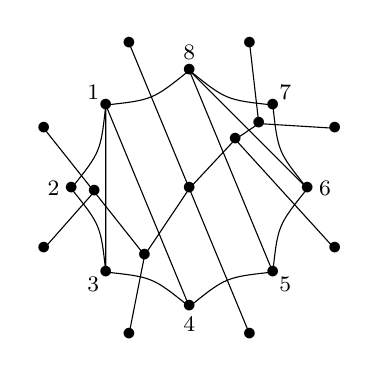
\begin{tikzpicture}[rotate=67.5,baseline=(current bounding box.east)]
	\begin{scope}
	\drawpolypart{8}{1.5}
    \drawnumbersshift
    \drawchord{1}{4}
    \drawchord{1}{3}
    \drawchord{5}{8}
    \drawchord{6}{8}
 \draw (0,0) node {$\bullet$};
\draw (-1,.2) node {$\bullet$};	
\draw (-.5,1.1) node {$\bullet$};
\draw (.8,-.3) node {$\bullet$};	
\draw (1.1,-.5) node {$\bullet$};
\draw(1.1,-.5) -- (.8,-.3) --(0,0)--(-1,.2) -- (-.5,1.1);
\foreach \i in {1,2,...,8} {
      \draw (45*\i:2) node {$\bullet$};
    }
\draw (45*1:2) --(0,0) -- (45*5:2);
\draw (45*6:2) -- (.8,-.3);
\draw (45*8:2) -- (1.1,-.5) -- (45*7:2);
\draw (45*2:2) -- (-.5,1.1) -- (45*3:2);
\draw (45*4:2) -- (-1,.2);
	\end{scope}
	\end{tikzpicture} \rightarrow 
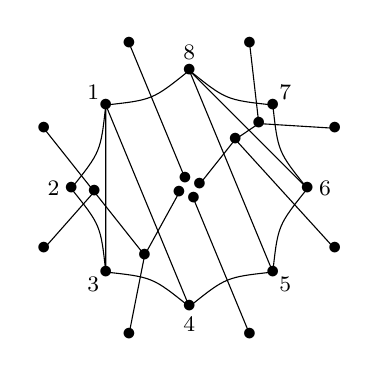
\begin{tikzpicture}[rotate=67.5,baseline=(current bounding box.east)]
	\begin{scope}
	\drawpolypart{8}{1.5}
    \drawnumbersshift
    \drawchord{1}{4}
    \drawchord{1}{3}
    \drawchord{5}{8}
    \drawchord{6}{8}
 \draw (.1,.1) node {$\bullet$};
\draw (.1,-.1) node {$\bullet$};
\draw (-.1,-.1) node {$\bullet$};
\draw (-.1,.1) node {$\bullet$};
\draw (-1,.2) node {$\bullet$};	
\draw (-.5,1.1) node {$\bullet$};
\draw (.8,-.3) node {$\bullet$};	
\draw (1.1,-.5) node {$\bullet$};
\draw(1.1,-.5) -- (.8,-.3) --(.1,-.1); 
\draw (-.1, .1) --(-1,.2) -- (-.5,1.1);
\foreach \i in {1,2,...,8} {
      \draw (45*\i:2) node {$\bullet$};
    }
\draw (45*1:2) --(.1,.1);
\draw (-.1, -.1) -- (45*5:2);
\draw (45*6:2) -- (.8,-.3);
\draw (45*8:2) -- (1.1,-.5) -- (45*7:2);
\draw (45*2:2) -- (-.5,1.1) -- (45*3:2);
\draw (45*4:2) -- (-1,.2);
	\end{scope}
	\end{tikzpicture}
\eas



To see uniqueness, consider a different maximal decomposition of $\tau(W)$. This induces a splitting on $T(W)$, where each connected component of the new decomposition corresponds to a subtree. Call this forest $f'$. Since $f' \neq f$, there are two trees, $t$ and $t'$ in $f$ and $f'$ that are distinct, but share at least one edge of $T(W)$. Since $f'$ is also maximal, $t'$ is not a subtree of $t$. Therefore, the edges of $t'$ can be found in at least two trees in the forest $f$. In particular, there is a vertex $v$ in $t'$ that corresponds to a split vertex of $T(W)$ in the original decomposition.
This implies that $v$ has valence greater than $3$ in $T(W)$, and thus the corresponding face of $\tau(W)$ is not a triangle. In other words, the decomposition corresponding to $f'$ is not a triangulation. 
\end{proof}

\begin{cor} \label{maxtriangdisjointcor}
Given a maximal decomposition of $\tau(W)$, the maximal triangulated pieces are edge disjoint.
\end{cor}

\begin{proof}
Consider any two distinct maximal triangulated pieces of $\tau(W)$. These two pieces correspond to subtrees of $T(W)$ and intersect, at most, at a vertex in the interior of $\tau(W)$. Since the subtrees corresponding to the maximal triangulated pieces are edge disjoint, and the edges of $T(W)$ correspond to the edges of $\tau(W)$, this forces the maximal triangulated pieces to be edge disjoint as well.
\end{proof}


We are now in a position to relate the triangulated pieces of $\tau(W)$ to exact subdiagrams of $W$.

Every triangulated piece $t$ of an admissible Wilson loop diagram $W$ corresponds to a subdiagram of $W$ by taking the set of propagators $P$ corresponding to edges of $t$ and then taking the subdiagram $W_P = (P, V(P))$.  Conversely, given a subdiagram $W_P = (P, V(P))$ of $W$ we can obtain a subgraph of $\tau(W)$, called $t$, as follows:
\begin{itemize}
\item The vertex set of the subgraph $t$ is
  \begin{itemize}
  \item the vertices of $\tau(W)$ corresponding to edges of $W$ defined by cyclically consecutive elements of $V(P)$ as a subset of $[n]$
  \end{itemize}
\item The edge set of the subgraph is
  \begin{itemize}
  \item the edges of $\tau(W)$ corresponding to propagators of $P$
  \item along with the outer edges of $\tau(W)$ for which both their end points are in the vertex set
  \end{itemize}
\end{itemize}
Note that the subgraph $t$ depends on how the propagators of $P$ sit inside $[n]$, not on how they sit in $W_P$ itself.  In particular $t$ is not the subgraph of $\tau(W)$ consisting only of edges corresponding to propagators of $P$. 


\begin{lem}\label{lem triang to exact}
  Let $W$ be an admissible Wilson loop diagram and $\tau(W)$ its polygon partition.  The triangulated pieces of $\tau(W)$ correspond to the exact subdiagrams of $W$ using the correspondence described above.
\end{lem}

\begin{proof}
Let us first record a few standard facts about polygon triangulations (that is, about triangulations with all vertices on the outer face).  If such a triangulation has $n$ vertices then it has $n$ edges on the polygon (that is, on the outer face) and $n-3$ edges which are not.  No planar graph with the same vertices and the same outer face can have more edges than the triangulation, and every such simple graph with $n-3$ edges off the outer face is a triangulation.

Since $W$ is admissible, by Lemma \ref{tausimpleplanarlem} $\tau(W)$ is a simple graph. Let $t$ be a triangulated piece of the decomposition of $\tau(W)$ given in Lemma \ref{decompositionlem}; note that $t$ cannot be equal to $\tau(W)$ by the definition of admissible diagrams.

If $t$ has 2 vertices then $t$ corresponds to a propagator that connects two non-adjacent edges. Therefore, the trivial triangulation is a trivial exact subdiagram.

Now suppose that $t$ has $m>2$ vertices.  We count how many edges of $t$ are not on the outer face of $\tau(W)$.  These are exactly the edges of $t$ defined by propagators of $W$. Consider the intersection of $t$ with the outer face of $\tau(W)$: this is a possibly disconnected subgraph of the polygon of $\tau(W)$ and this subgraph has $m$ vertices. Call this new subgraph $S$, and let $j$ be the number of connected components of $S$.   To join the components of $S$ into the outer face of $t$, $t$ must have $j$ edges in its outer face which are not in the outer face of $\tau(W)$.  Furthermore $t$ has $m-3$ edges not in its outer face and so also not in the outer face of $\tau(W)$.  Thus there are $m-3+j$ edges of $t$ not in the outer face of $\tau(W)$.

Each of these $m-3+j$ internal edges corresponds to a propagator in $W$; call this set of propagators $P$.  Next we count the size of $V(P)$.  Each of the $m$ vertices in the outer face of $t$ corresponds to an edge of $W$. These $m$ edges define $j$ connected components of the outer polygon of $W$. Thus the set $V(P)$ has $m+j$ vertices.  In other words, 
\[|V(P)| = m+j = |P| +3\;.\]
Thus the subdiagram $(P,V(P))$ defined by $t$ is exact.


Conversely, suppose we have an exact subdiagram $(P, V(P))$ of $W = (\cP, [n])$ supported on $|V(P)| = |P|+3$ vertices, and let $t$ be the subgraph of $\tau(W)$ corresponding to $(P,V(P))$.

Suppose $|P|=1$. Let $p$ be the element of $P$. The exactness condition on $(P, V(P))$ says that the four supporting vertices of $p$ are distinct.  If the support of $p$ is four consecutive vertices, then $V(p)$ defines three consecutive boundary edges of $W$, so $t$ is a single triangle, hence a triangulated piece.  If the support of $p$ is not four consecutive vertices, then the vertices which are the ends of $t$ are separated by at least two vertices along the cycle.  This implies that $t$ is a trivial triangulated piece.

Now suppose $|P|>1$.  Let $j=|P|$, $m=|V(P)|$, and 
suppose that the set $V(P)$ defines $c$ disjoint cyclic intervals of $[n]$. Then $t$ has $m-c$ vertices.  If $t$ were a triangulation, $t$ would have $j -c$ internal edges.

The graph $t$ has $j$ edges that come from propagators, and $m - 2c$ edges that come from the boundary polygon of $\tau(W)$. Since $t$ has $m-c$ vertices, it has $m-c$ external edges, of which $c$ come from propagators. Therefore, of the $j$ edges of $t$ that come from propagators, $j-c$ are internal to the connected component. Therefore, $t$ is a triangulated piece.


%  The statement of the lemma then follows form the fact that inclusion is preserved under $\tau$ and so maximality also corresponds under $\tau$.
\end{proof}





To avoid the issue of exact diagrams being subdiagrams of other exact subdiagrams (for instance, any subdiagram $(q, V(q))$, for $q \in \cP$ is exact), we introduce the notion of maximal exact subdiagrams.

\begin{dfn}
An exact subdiagram $(P, V(P))$ is a {\em maximal exact subdiagram} of $W$ if there is no other exact subdiagram $(Q, V(Q))$ in $W$ that contains $(P,V(P))$ as a strict subdiagram.
\end{dfn}


\begin{cor} \label{uniqueproppartitioncor}
Any admissible Wilson loop diagram $W = (\cP, [n])$ can be uniquely decomposed into maximal exact subdiagrams. These maximal subdiagrams partition $\cP$.
\end{cor}

\begin{proof}
Combining Lemmas \ref{decompositionlem} and \ref{lem triang to exact} yields the unique decomposition into maximal exact subdiagrams, and Corollary \ref{maxtriangdisjointcor} ensures that no propagator appears in more than one subdiagram in this decomposition. Since the chord edges of $\tau(W)$ correspond to the propagators of $W$, the decomposition of $\tau(W)$ induces a partition of $\cP$.
\end{proof}

\subsection{Matroidal properties of exact subdiagrams \label{sec: exact diagram matroidal props}}

Since Corollary \ref{uniqueproppartitioncor} allows us to decompose any admissible Wilson loop diagram into a collection of maximal exact subdiagrams, in this section we examine the matroid properties of exact subdiagrams more closely. In this section, we show prove two results:
\begin{enumerate}
\item The matriod assoicated to an exact subdiagram of $W$ can be written as a contraction of the matroid $M(W)$ by the complementary propagator flat (Theorem \ref{exact diagrams contractions}). 
\item The matroid associated to an exact subdiagram is uniform (Theorem \ref{exactuniformthm} ).
\end{enumerate}

We begin by proving some useful facts about propagator flats, and flats of matroids associated to admissible Wilson loop diagrams more generally.

\begin{comment}


\begin{dfn}\label{def prop flat} 
Let $W = (\cP,[n])$ be an admissible Wilson loop diagram and $P \subseteq \cP$. The set $F(P) := V(P^c)^c$ is called the {\em propagator flat} of $P$.
\end{dfn}
Thus in Lemma \ref{contractsubdiaglem} above we would contract $M(W)$ by the propagator flat $F(P^c)$ of the {\em complement} of $P$ in order to study $(P,V(P))$. The justification for this notation is given by (1) of the next lemma: the set $F(P)$ consists of vertices which {\em only} support propagators in $P$ (or no propagators at all).

\begin{lem}\label{lem properties of prop flats} \sanote{do we need the first 2? They follow directly from the definition 1.2. Do we use them later?}
Let $F(P)$ be a propagator flat as defined above. Then
\begin{enumerate}
\item $F(\emptyset)$ is exactly the set of vertices which support no propagators, while for $P \neq \emptyset$ we have \[F(P) = \big(V(P) \setminus V(P^c)\big) \cup F(\emptyset).\] \note{updated (1) to match new definition of $F(P)$; }
\item If $Q\subseteq P$ then $F(Q) \subseteq F(P)$.
\item $F(P)$ is a flat of $M(W)$, thus justifying the name ``propagator flat''.
\end{enumerate}
\end{lem} \sanote{I'd like to attach this to the "generic facts about matroids" in lemma 2.2?}
\begin{proof}
The proof of (1) and (2) are routine applications of the definition and are omitted.

To prove (3), we need to show that $F(P)$ is maximally dependent. If $F(P) = [n]$ then this is automatic, so suppose not and let $v \in [n] \setminus F(P)$. In other words, $v \in V(P^c)$ and so $v$ supports some propagator $q \not\in P$.  Let $S \subseteq F(P)$ be an independent set of maximal size. Then $\Prop(S) \subseteq P$ by (1), and no subset of $S$ supports fewer propagators than the number of vertices it contains (this is the definition of an independent set in $M(W)$). Since $v$ supports a new propagator $q \not\in P$, the set $S \cup \{v\} \subseteq F(P) \cup\{v\}$ also satisfies this independence condition. Thus $\rk(F(P) \cup\{v\}) = \rk(F(P)) + 1$, as required.
\end{proof}


\end{comment}

\begin{lem} \label{lem decompose flat}Let $F$ be a flat in $M(W)$, and let $C \subseteq F$ be the union of all circuits contained in $F$. Then the following are true:
\begin{enumerate}
\item $C = F(\Prop (C))$, i.e. $C$ is a propagator flat.
\item $F \setminus C$ is an independent set. Furthermore, If $F\setminus C$ is an independent flat if and only if $F(\emptyset) = \emptyset$, that is $W$ has no non-supporting vertices.  
\end{enumerate}
\end{lem}

\begin{proof}
(1) If $F$ is an independent flat, then $C = \emptyset$ and the statement is trivially true. Now suppose that $F$ is a dependent set, so $C$ is non-empty.

Let $v \in C$. Clearly $\Prop(v) \subseteq \Prop(C)$. Since $F(P)  = V(P^c)^c$, we have $F(\Prop(v)) \subseteq F(\Prop(C))$. Since $v \in F(\Prop(v))$ by the definition of propagator flat, we have $v \in F(\Prop(C))$ as required, and $C \subseteq F(\Prop(C))$. 

Now suppose there exists some $w \in  F(\Prop(C)) \setminus C$. Let $B$ be an independent subset of $C$ of maximal rank; we first show that $B \cup \{w\}$ is a dependent set in $M(W)$. By Lemma \ref{lem facts about WLD matroids}, \bas |\Prop(C)| = \rk(C) = |B| = \rk(B) .\eas Since $B \subseteq C$ implies that  $\Prop(B) \subseteq \Prop(C)$, this implies that $\Prop(B) = \Prop(C)$. Furthermore, since $w \in F(Prop(C)$, $\Prop(B\cup w) \subseteq \Prop(B)$. By Lemma \ref{lem facts about WLD matroids} $\rk (B \cup w) \leq \min\{|B\cup w|, |\Prop(B\cup w)|\}$, and therefore $\rk (B \cup w) < |B\cup w|$. That is, $B\cup w$ is a circuit in $F(\Prop(C))$. Therefore, $B \cup w \subset C$, leading to a contradiction.


For part (2), first note that $F \setminus C$ is automatically independent as it contains no circuits.

Note that since $F(\emptyset)$ has rank $0$, $F(\emptyset)$ is contained in every flat of $W$. Therefore, if $F(\emptyset) \neq \emptyset$, then $F\setminus C$ cannot be a flat. 

If $F(\emptyset) = \emptyset$, for any $e \not\in F$, we certainly have $\rk((F\setminus C)\cup\{e\}) = \rk(F\setminus C) +1$ since $F$ is a flat. Now let $e \in C$, and suppose that $\rk((F\setminus C)\cup\{e\}) = \rk(F\setminus C)$. This implies that $(F\setminus C)\cup \{e\}$ is dependent, and hence contains a circuit, $S$. Since $F(\emptyset) = \emptyset$, this circuit must contain at least two elements but this contradicts the fact that $C$ was the union of all circuits in $F$. 

Thus $\rk((F\setminus C)\cup \{e\}) = \rk(F\setminus C) + 1$ for any $e \not\in F\setminus C$, and hence $F\setminus C$ is a flat.
\end{proof}

\begin{cor} \label{classifyflats}
If $F$ is a flat of a Wilson loop diagram, it can be written as the disjoint union of a cyclic propagator flat and an independent set and the set of non-supportive vertices. \end{cor}
 
In particular, any propagator flat can be written as a union of a cyclic propagator flat, an independent set and $F(\emptyset)$ for the appropriate Wilson loop diagram.

Next we examine properties of propagator flats associated to the complement of Wilson Loop diagrams.
%Finally, we note the differences between subdiagrams of Wilson loop diagrams, and restrictions or cotractions of the associated matroids.

%Given any matroid, one may restrict it to a subset of the base set. The bases of the restricted matroid come from intersecting bases of the original with the subset. It is worth noting that a the matroid defined by a subdiagram is different from the restriction of the matroid of a Wilson loop diagram to a set of vertices.

% \begin{dfn} \label{restrictiondfn}
% For $W = (\cP, [n])$, the restricted diagram, $W|_V$ is the matroid defined by only looking at the vertices $V \subset [n]$.
% \end{dfn}

% The key difference between a subdiagram and a restriction is that the propagator support function does not change in the case of restriction, while it may in the case of a subdiagram. In particular, for $v \in V$, $\Prop_W(v) = \Prop_{W|_V}(v)$, while $\Prop_{(P, V(P))} (v) = \Prop_W(v) \cap P$.

% A subdiagram is more closely related to a contracted matroid.



\begin{lem} \label{maxexactcomplementrank}
Let $W = (\cP, [n])$ be a Wilson loop diagram, and $P \subseteq \cP$. Then: \begin{enumerate}
\item If $(P,V(P))$ is an exact subdiagram in $W$, then $F(P^c)$ is not an independent flat.
\item If $(P,V(P))$ is a maximal exact subdiagram in $W$, then $F(P^c)$ is a cyclic flat.                                                                                                                                                                                                                                                                                                                                                                                                                                                                                                                                                                                                                                                                                                                                                                                                                                                                                                                                                                          \item If $(P,V(P))$ is an exact subdiagram in $W$, then $\rk(F(P^c)) = |P^c|$.
\end{enumerate}
\end{lem}


\begin{proof}
%Note that $|P^c|$ is always an upper bound on the rank of $F(P^c)$ for any $P \subseteq \cP$, since $F(P^c)$ supports at most $P^c$ propagators (see Remark \ref{alt F(P) rmk}), and $\rk (F(P^c)) = \min\{ |F(P^c)|, |\Prop(F(P^c))|\}$. To show equality, we need to show that $F(P^c)$ is not an independent set and that $\Prop(F(P^c)) = P^c$. 

First note that if $(P,V(P))$ is exact then the admissiblity of $W$ guarantees that $F(P^c)$ is a non-empty flat. That is, $V(P) \subsetneq [n]$.

Since $W$ is admissible, we have $n \geq |\cP| + 4$. Rewriting this as
\[|V(P)| + |F(P^c)|  \geq  |P| + |P^c| +4,\]
and combining it with the fact that $|V(P)| = |P| + 3$ (from the exactness of $(P,V(P))$), we obtain
\begin{equation}\label{eq F is dependent}|F(P^c)| > |P^c| \;.\end{equation}
Equation \eqref{eq F is dependent} is therefore saying that $F(P^c)$ supports fewer propagators than the number of vertices it contains, i.e. $F(P^c)$ is not an independent set.

For part (2), suppose that $(P, V(P))$ is a maximal exact subdiagram. By Corollary \ref{classifyflats} we can decompose $F(P^c)$ as
\begin{equation}\label{eq decompose F}V(P)^c = F(P^c) = C \sqcup S = F(\Prop(C)) \sqcup S,\end{equation}
where $C$ is the largest cyclic flat contained in $F(P^c)$ and $S$ is an  independent set. Note that $C$ must be non-empty since $F(P^c)$ is non-empty and dependent (by part (1)).

Since $S$ is an independent set, $\rk(S) = |S|$, and every element of $S$ is independent of $C$, $\rk\big(F(P^c)\big) = \rk(C) + \rk(S)$. By Lemma \ref{lem facts about WLD matroids}(2), \ba \rk(S) = \rk\big(F(P^c)\big) -  \rk(S) \leq |P^c| - \rk(C) \;. \label{increasingrank} \ea

Let $Q^c = \Prop(C)$. Then $C = F(Q^c)$ and, by Lemma \ref{lem facts about WLD matroids}(1), $\rk(C) = |Q^c|$. By equation \eqref{increasingrank}, \ba |P| + |S| \leq |P| + |P^c| - \rk(C) = |\cP| - |Q^c| = |Q| \;. \label{Qsizebound}\ea From equation \eqref{eq decompose F}, \bas |V(Q)| = V(P) \sqcup S = C^c = F(\Prop(C))^c = F(Q^c)^c = V(Q) \;. \eas Combining this with equation \eqref{increasingrank} gives \ba |V(Q)| = | V(P) | + |S| = | V(P) | + 3 + |S| \leq |Q| +3 \;. \label{Q defines exact}\ea Since $W$ is admissible, one must have $V(Q) = |Q| +3$, that is the subdiagram $(Q, V(Q))$ is exact.

Next, note that \bas C = F(Q^c) = V(Q)^c \subset F(P^c) = V(P)^c \;,\eas which implies that $P \subseteq Q$. That is, $(P, V(P))$ is a subdiagram of $(Q, V(Q))$. Since $(P, V(P))$ is maximally exact by hypothesis, and $(Q, V(Q))$ is exact by \eqref{Q defines exact}, we are forced to have $S = \emptyset$. Therefore, $F(P^c)$ is a cyclic flat.

To see (3), first note that the second point of this Lemma, combined with Lemma \ref{lem facts about WLD matroids} that
\bas\rk(F(P^c)) = |\Prop(F(P^c))| = |P^c|.\eas 

To prove this in the general case, let let $(R,V(R))$ be an exact subdiagram that is not maximal and $P$ be the maximal exact subdiagram containing it. That is, $R \subsetneq P$.

Since $R \subset P$, $V(P) = V(R) \sqcup S$, where $S = V(P) \setminus V(R)$. Since $P$ and $R$ both define exact subdiagrams, we may write $|V(P)| = |V(R)| + |P \setminus R|$, where $S$ is a vertex set of size $|P \setminus R|$ with $(P \setminus R \subset \Prop(S)$. Since  $|S| = |V(P) \setminus V(R)| = |P \setminus R| \leq |\Prop(S) |$, by Lemma \ref{lem facts about WLD matroids}, $\rk(S) = |S|$, implying that $S$ is independent. Taking the complements, we may write \bas F(R^c ) = F(P^c) \sqcup S \;.\eas Taking the rank of both sides, \bas \rk(F(R^c )) = \rk(F(P^c) \sqcup S ) \leq \rk(F(P^c)) + |S| = |P^c| + |\Prop(S)| \leq |R^c| \;.\eas Combining this with \eqref{eq F is dependent} gives the desired result.

\end{proof}

We are now ready to show that any exact subdiagram $(P, V(P)$ of $W$ can be written as a contraction of $M(W)$ by $F(P^c)$. We begin with a definition.

\begin{dfn}\label{matroid contraction}
Let $M = (E,\cB)$ be a matroid, and $S \subseteq E$. The {\em contraction} of $M$ by $S$ is the matroid $M/S = (E \setminus S, \cB / S)$, where
\[\cB / S = \{B \setminus S \ \big| \ |B\cap S | \text{ is maximal amonst all }B \in \cB\}.\]
\end{dfn}

In \cite{wilsonloop}, Agarwala and Amat show that certain subdiagrams of $W$ can be realized as contractions of $M(W)$:

\begin{lem} \label{contractsubdiaglem} \cite[Theorem 3.33]{wilsonloop} 
Let $W = (\cP, [n])$ be an admissible Wilson loop diagram and $P \subseteq \cP$. If the set $V(P)^c$ has rank $|P^c|$, then the matroid defined by the subdiagram $(P, V(P))$ is equal to the contraction $M(W)/V(P)^c$.
\end{lem}

\begin{thm} \label{exact diagrams contractions}
If $(P, V(P)$ is an exact subdiagram of of $W$, one may write \bas M\big((P, V(P))\big) = M(W)  / F(P^c) \;.\eas 
\end{thm}

\begin{proof}
This follows from Lemma \ref{matroid contraction}. Lemma \ref{maxexactcomplementrank} shows that the supports of exact subdiagrams satisfy the conditions of this lemma.
\end{proof}

\begin{rmk} \label{remark exact dual restiction}
Let $M^*$ denote the dual of a matroid. The the dual of a contraction of a matroid is the same as the restriction of the dual matroid by the complement: \bas M / S = M^*|_{S^c} \;.\eas Then Theorem \ref{exact diagrams contractions} implies that, for $(P, V(P))$ an exact subdiagram of $W$ \bas M\big((P, V(P))\big) = M(W)  / F(P^c) = M(W)^*|_{V(P)} \;.\eas
\end{rmk}

Matroids coming from exact subdiagrams have an especially nice structure, namely, they are uniform. Recall from Section \ref{sec matroid background} that a uniform matroid of rank $r$ is one in which all sets of size $ \leq r$ are independent.

\begin{thm} \label{exactuniformthm}
Let $W':= (P, V(P))$ be a subdiagram of an admissible Wilson loop diagram $W= (\cP, [n])$. Then $W'$ is an exact subdiagram if and only if $M(W')$ is a uniform matroid of rank $|P|$.
\end{thm}

\begin{proof}
It follows directly from the definitions that a matroid of rank $r$ is uniform if and only if all circuits have rank $r$; we therefore focus on the circuits of $M(W')$.

We prove the following claim: $W'$ is exact if and only if $V(P)$ contains no circuits $C$ with $\rk C< |P|$ in $(P, V(P))$. Since $\rk(M(W'))$ is bounded above by $|P|$, the result follows.

Suppose $C \subseteq V(P)$ is a circuit of rank $m < |P|$; by Lemma \ref{lem facts about WLD matroids}, we know that $|\Prop_{W'}(C)| = m$ as well, where the subscript to $\Prop$ specifies the diagram we are working in.  Observe that $\Prop_{W'}(C)\subseteq P$ by definition. The set $P \setminus \Prop_{W'}(C)$ is thus nonempty, and we can consider the subdiagram $W'':= (P\setminus \Prop_{W'}(C),V(P\setminus\Prop_{W'}(C))$. By the density condition on subdiagrams of admissible diagrams, we have
\[|V(P\setminus\Prop_{W'}(C))| \geq |P\setminus\Prop_{W'}(C)| + 3.\]
It is easy to verify that $V(P\setminus\Prop_{W'}(C)) \subseteq V(P)\setminus C$; since $C \subseteq V(P)$ and $\Prop_{W'}(C) \subseteq P$, we can therefore rewrite the previous inequality as
\[|V(P)| - (m+1) \geq |V(P\setminus\Prop(C))| \geq |P| - m + 3.\]
Simplifying, we obtain $|V(P)| \geq |P| + 4$, i.e. $(P,V(P))$ is not an exact diagram.

Conversely, suppose that $W'$ is not exact and for a contradiction suppose also that $M(W')$ is uniform of rank $|P|$.  Take $p \in P$.  Then $|V(P)\setminus V(p)| = |V(P)| - 4 \geq |P|$ by non-exactness.  By uniformity there is an independent set of size $|P|$ in $V(P)\setminus V(p)$.  This is impossible because the submatrix corresponding to this independent set has $|P|$ rows but the one corresponding to $p$ is all $0$ one of them is all 0 so it cannot be full rank.
%suppose that $(P,V(P))$ is not exact, i.e. $|V(P)| \geq |P| +4$. We have 
%\[|V(P)| - (m+1) \geq |P| - m + 3\]
%as above, but \hlfix{we need to know that $P\setminus\Prop(C)$ is non-empty before we can complete the argument.}{and if we knew this, it would be immediate that $\rk(C) < |P|$}
\end{proof}

We now make a few observations about the geometry of matroids defined by exact diagrams.

In \cite{wilsonloop}, the authors show that all admissible Wilson loop diagrams correspond to positroids. That is, they correspond to matroids that can be represented by elements of the positive Grassmannians $\Gr(|\cP|, n)$. Any positroid of rank $k$ on $n$ elements defines a subspace of the positive Grassmannians $\Gr(k, n)$, namely the points which represent it. These subspaces give a CW structure on $\Gr(k,n)$, with each positroid defining a cell. 

\begin{dfn}
Given a Wilson loop diagram $W = (\cP, [n])$, define the positroid cell associated to a Wilson loop diagram, $\Sigma(W)$, to be the cell in the CW complex on $\Gr(|\cP|, n)$ defined by the positroid $M(W)$.
\end{dfn}

With this definition in mind, we have the following corollary:

\begin{cor}
Let $(P, V(P))$ be an exact subdiagram of $W$. The matroid associated to this subdiagram corresponds to the top dimensional cell in $\Gr(|P|, |V(P)|)$.
\end{cor}

\begin{proof}
The unique top dimensional cell of $\Gr(|P|, |V(P)|)$ is defined by all points in $\Gr(|P|, |V(P)|)$ such that all Plucker coordinates are strictly greater than $0$. Since $(P, V(P))$ is an exact subdiagram, this all $|P| \times |P|$ minors are non-zero. Intersecting these with the cases with the positive Grassmannians demands that all minors be strictly positive.
\end{proof}

%Since the matroid defined by the subdiagram $(P , V(P))$ is not the same as the matroid associated to $W_{V(P)}$, one cannot say that the $W_{V(P)}$ is a uniform matroid. In fact, for any subset $U \subset V(P)$, $\rk_{W_{V(P)}}(U) \geq \rk_{(P , V(P))}(U)$. This is because adding propagators to vertices can only increase the rank. In particular this implies that, for any subset $U \subset V(P)$, if $|U| \leq |P|$, then $U$ is independent in both the restricted matroid $W_{V(P)}$, and the original, $W$.



\subsection{Matroids and equivalent diagrams \label{sec: matroids and equivalence}}
\note{Si\^an postponed reading this section until the earlier ones are fixed.}
Now we are ready to prove the main results of this section, namely that two Wilson loop diagrams define the same matroid if and only if they are equivalent (Theorem \ref{same matroid iff equiv}). We also {\color{violet}count the number of equivalence classes amongst Wilon Loop diagrams with $n$ vertices and $k$ propagators and} give a formula for the number of Wilson loop diagrams in a given equivalence class (Corollary \ref{number of equiv diagrams}), completing the characterization of the correspondence between Wilson Loop diagrams and matroids starting in \cite{wilsonloop}.

\begin{thm}\label{same matroid iff equiv}
Let $W= (\cP, [n])$ and $W'= (\cP', [n])$ be two Wilson Loop diagrams. They define the same matroid if and only if $W \sim W'$.
\end{thm}

\begin{proof}
One direction has been proved in \cite[Theorem 1.18]{wilsonloop}, but we give a different proof here to be consistent with the method of this document.

Assume that $W$ and $W'$ are equivalent. Without loss of generality, write $W = (P \cup R, [n])$ and $W' = (P \cup R', [n])$, where $P \subset \cP \cap \cP'$ and $(R, V(R))$ and $(R', V(R'))$ are two maximally exact subdiagrams, with $R \neq R'$, but $V(R) = V(R')$. If this is not the case, one may always find a family of diagram, $\{W_i\}$ satisfying this condition and forming a transitive chain connecting $W$ to $W'$ in the equivalence class.

Let $U \subset V(R)$ be any subset of size $|U| = |R|$. Since $(R, V(R))$ defines a uniform matroid, by Lemma \ref{exactuniformthm}, the set $U$ is independent in the subdiagram $(R, V(R))$, and thus in $W$. The complementary set $F(P)$ is a flat of maximal rank by lemma \ref{maxexactcomplementrank} ($\rk(F(P)) = |P|$). Let $B \subset F(P)$ be a maximal indpendent set ($\rk B = |P|$) in $F(P)$. Since $F(P)$ is a flat, adding any element of $V(R)$ to $B$ increases the rank. Therefore, any basis of $W$ can be written as $B \cup U$ for some $B$ and $U$ of the form indicated. However, since $F(P)$ is common to both $W$ and $W'$, and $V(R) = V(R')$, any any basis of $W'$ can also be written $B \cup U$. Thus both matroids have the same bases sets, proving that they are the same.

For the converse, assume that the matroids associated to $W$ and $W'$ are the same: $M(W) = M(W')= M$. Let $\mathcal{R} = \{(P_i, V(P_i)\}_{i=1}^k$ and $\mathcal{R}' = \{(P'_i, V(P'_i)\}_{i=1}^l$ be the sets of maximally exact subdiagrams of $W$ and $W'$. Write $F_i = F(P_i^c)$ and $F'_i = F(P^{'c}_i)$ to be the complementary cyclic flats. By Theorem \ref{exactuniformthm} and Theorem \ref{exact diagrams contractions},  $M/F_i$ and $M/F_i'$ are uniform matroids. Since, by Theorem \ref{exactuniformthm}, any subset $V$ of $M$ such that $M/(V^c)$ is uniform defines an exact subdiagram of both $W$ and $W'$. If $U \subset V$ are two such thsets, then the corresponding exact subdiagrams are also subsets. Therefore, $|\mathcal{R}| = |\mathcal{R}'|$, and we write $V(P_i) = V(P'_i)$, after possibly reindexing $\mathcal{R}$ and $\mathcal{R}'$.

Since the sets of propagators defining maximal exact subdiagrams partition $\cP$, by Lemma \ref{uniqueproppartitioncor}, write $\cup_{i = 1}^k P_i = \cup_{i = 1}^k P'_i = \cP$. Reorganize the vertex sets of maximal exact subdiagrams as follows: \ba \cup_{P_i \not \in \mathcal{R}'} V(P_i) = V(\cup_{P_i \not \in \mathcal{R}'} P_i)  = F(\cup_{P_i \in \mathcal{R}'} P_i)^c\label{vertexsets}\; .\ea The final flat may, of course, be empty.

Thus, we have partitioned the vertices of $W$ and $W'$ into two complementary sets. The first, $ \cup_{P_i \not \in \mathcal{R}'} V(P_i)$,  is comprised of the union of supports of maximal exact subdiagrams whose propagators differ between $W$ and $W'$. The second, $ F(\cup_{P_i \in \mathcal{R}'} P_i)$,  is the propagator flat of all propagators in common between $W$ and $W'$.

Without loss of generality, assume that $|\mathcal{R}| = |\mathcal{R}'| = 1$. Then the two Wilson loop diagrams are equivalent. If  $|\mathcal{R}| = |\mathcal{R}'| > 1$, then one may define a family of Wilson loop diagrams, $W_0$ to $W_k$ defined such that $W_0 = W$ and $W_i$ is derived from $W_{i-1}$ by replacing the propagator set $P_i$ with $P'_i$. In this manner, $W' = W_k$ and $W_i \sim W_{i+1}$, making $W \sim W'$.
\end{proof}

Since there is a unique way to decompose $W$ into maximal exact subdiagrams, it is logical to ask how many diagrams there are in an equivalence class. It is a classical fact the the number of triangulations of an $n$-gon is the $n-2$ Catalan number, namely $\frac{1}{n-1}\binom{2(n-2)}{n-2}$.  Thus we can count the number of equivalent diagrams. [CITATION?]

\begin{cor}\label{number of equiv diagrams}
  Let $W$ be an admissible Wilson loop diagram where the sizes of the supports of the nontrivial maximal connected exact subdiagrams are $n_1, n_2, \ldots, n_j$.  Then the number of admissible Wilson loop diagrams equivalent to $W$ (including $W$ itself) is
  \[
  \prod_{i=1}^{j} \frac{1}{n_i-1}\binom{2(n_i-2)}{n_i-2}
  \]
\end{cor}

In this section we have characterized the correspondence between Wilson loop diagrams and positroids, showing that Wilson Loop diagrams define the same matroid if and only if they are equivalent (Theorem \ref{same matroid iff equiv}). Corollary \ref{number of equiv diagrams} enumerates the fibres of the map from Wilson Loop diagrams to positroids. {\color{violet} By counting the number of equivalence classes (Theorem \ref{}), we enumerate the number of positroids defined by Wilson Loop diagrams. In section \ref{}, Theorem \ref{}, we show that each Wilson Loop diagram with $n$ vertices and $k$ propagators define a positroid cell of dimension $3k$. Comparing the result of Theorem \ref{} to the number of positroid cells of a particular dimension in $\Grtnn(n, k)$, [CITE AND FIND FORMULA HERE], we see that \emph{Wilson loop diagrams do not map onto all positroids of the correct dimension.}} 



\begin{comment}
\subsection{Counting exact subdiagrams}


\begin{dfn}
  Say two admissible Wilson loop diagrams $W_1$ and $W_2$ are \emph{triangulation-equivalent} if there is a bijection $\alpha$ between the set of triangulated pieces in the decomposition of $\tau(W_1)$ and the set of triangulated pieces in the decomposition of $\tau(W_2)$, where $t$ and $\alpha(t)$ have the same vertex set for all triangulated pieces $t$ of $\tau(W_1)$.
\end{dfn}

***draw an example***

\begin{thm}
  Two admissible Wilson loop diagrams have the same matroid iff they are triangulation equivalent
\end{thm}

Again do I want matroid or positroid in this theorem?

\begin{proof}
  By Lemma~\ref{lem triang to exact} two admissible Wilson loop diagrams are triangulation equivalent iff their decompositions into maximal connected exact subdiagrams have matching supports, that is if they are equivalent.
  Theorem~\ref{thm orig equiv} then gives the result.
\end{proof}



\end{comment}

\section{Geometry of Wilson Loop diagram}\label{sec GN algorithm}


Since Wilson loop diagrams correspond to positroids, it is natural to study the subspace of $\Gr(|\cP|, n)$ they define. 

[words about what's in this section]

Throughout this section, $W = (\cP,[n])$ is an admissible Wilson loop diagram with $k$ propagators.

\subsection{Background}\label{sec:positroid background}

[positroids]

Let $\binom{[n]}{k}$ be the set of all $k$-subsets of the cyclically ordered set $[n]$.  For each $j \in [n]$, we can define a total order $\leq_j$ on the interval $[n]$ by
\[ j <_j j+1 <_j \dots <_j n <_j 1 \dots <_j j-1\;.\]
This in turn induces a total order on $\binom{[n]}{k}$, namely the lexicographic order with respect to $<_j$.  It also induces a separate partial order $\gale{j}$ on $\binom{[n]}{k}$ (the {\bf Gale order} \cite{Gale}), which is defined as follows: for 
\[A = \{a_1 <_j a_2 <_j \dots <_j a_k\} \text{ and } B = \{b_1 <_j b_2 <_j \dots <_j b_k\} \in \binom{[n]}{k},\] we define
\[A \gale{j} B \text{ if and only if } a_r \leq_j b_r \text{ for all }1 \leq r \leq k.\]
For example, in $\binom{[6]}{3}$ we have $\{2,5,6\}\gale{2} \{2,6,1\}$ but $\{2,5,6\}\not\gale{2}\{3,4,6\}$.


\begin{dfn}\label{def:grassmann necklace}
A {\bf Grassmann necklace} of type $(k,n)$ is a sequence $(I_1, \dots, I_n)$ of $n$ sets $I_i \in \binom{[n]}{k}$ such that for each $i \in [n]$:
\begin{itemize}
\item if $i \in I_i$, then $I_{i+1} = \big(I_i \backslash \{i\}\big) \cup \{j\}$ for some $j \in[n]$.
\item if $i \not\in I_i$, then $I_{i+1} = I_i$.
\end{itemize}
By convention, we set $I_{n+1} = I_1$.
\end{dfn}

By \cite[Theorem 17.1]{Postnikov}, the Grassmann necklaces of type $(k,n)$ are in 1-1 correspondence with the positroid cells in $\Gr(k,n)$.  This correspondence is given explicitly in \cite[Theorem 8]{Oh}: if $(I_1, \dots, I_n)$ is the Grassmann necklace associated to a positroid $M = ([n],\cB)$, then the bases of $M$ are exactly
\[\cB = \left\{J \in \binom{[n]}{k}\ :\ I_i \gale{i} J \ \forall i \in [n]\right\}.\]

\begin{dfn}\label{def:le diagram}
A {\bf Le diagram} is a Young diagram in which every square contains either a $+$ or a $0$, subject to the rule that if a square contains a $0$ then either all squares to its left (in the same row) must also contain a $0$, or all squares above it (in the same column) must also contain a $0$, or both.
\end{dfn}

By [ref], the set of all Le diagrams that fit within a $k\times(n-k)$ rectangle is in 1-1 correspondence with the positroid cells of $\Gr(k,n)$. The dimension of a positroid cell is equal to the number of $+$ squares in its Le diagram [ref].

The rows and columns of a Le diagram are labelled as follows: given a Le diagram fitting inside a $k\times (n-k)$ box, arrange the numbers $1,2, \dots, n$ along its southeast border, starting from the top-right corner. See Figure \ref{fig:row column numbering} for examples.

\begin{figure}[h!]
\[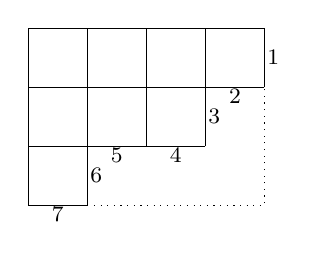
\begin{tikzpicture}[baseline=(current bounding box.east),scale=0.75]
\draw (1,0) grid (2,3);
\draw (2,1) grid (4,3);
\draw (4,2) grid (5,3);
\draw[dotted] (2,0) -- (5,0) -- (5,2);

\node at (5.15,2.5) {\footnotesize$1$};
\node at (4.5,1.85) {\footnotesize$2$};
\node at (4.15,1.5) {\footnotesize$3$};
\node at (3.5,0.85) {\footnotesize$4$};
\node at (2.5,0.85) {\footnotesize$5$};
\node at (2.15,0.5) {\footnotesize$6$};
\node at (1.5,-0.15) {\footnotesize$7$};
%\node at (0.5,-0.15) {\footnotesize$8$};
\end{tikzpicture}
\qquad \qquad
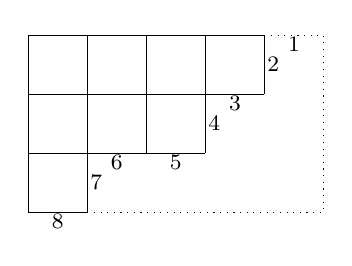
\begin{tikzpicture}[baseline=(current bounding box.east),scale=0.75]
\draw (1,0) grid (2,3);
\draw (2,1) grid (4,3);
\draw (4,2) grid (5,3);
\draw[dotted] (2,0) -- (6,0) -- (6,3) -- (5,3);

\node at (5.5,2.85) {\footnotesize$1$};
\node at (5.15,2.5) {\footnotesize$2$};
\node at (4.5,1.85) {\footnotesize$3$};
\node at (4.15,1.5) {\footnotesize$4$};
\node at (3.5,0.85) {\footnotesize$5$};
\node at (2.5,0.85) {\footnotesize$6$};
\node at (2.15,0.5) {\footnotesize$7$};
\node at (1.5,-0.15) {\footnotesize$8$};
%\node at (0.5,-0.15) {\footnotesize$9$};
\end{tikzpicture}
\]
\caption{Row and column numbering for a Young diagram with $k = 3$, $n = 7$ (left) and $k = 3$, $n = 8$ (right). The top left box in each diagram has coordinates $(1,7)$ (left diagram), $(2,8)$ (right diagram).}
\label{fig:row column numbering}
\end{figure}

An algorithm for constructing the Le diagram associated to a Grassmann necklace was given by Agarwala and Fryer in [ref]. Since we will make use of this algorithm in Section [ref] below, we summarise the process here.
\begin{algorithm}\label{alg:GN to Le} \ [ref]
Let $(I_1,\dots,I_n)$ be a Grassmann necklace of type $(k,n)$. Within a $k \times(n-k)$ square, draw the Young diagram whose rows are labelled by $I_1$ (as per the convention above).

For each $i$, $2 \leq i \leq n$:
\begin{itemize}
\item Write \[I_1 \setminus I_i = \{a_1 > a_2 > \dots > a_r\}, \quad I_i \setminus I_1 = \{b_1 < b_2 < \dots < b_r\},\]
where the inequalities denote the $<_1$ order (subscripts suppressed for clarity).
\item For $1 \leq j \leq r$ , place a $+$ in square $(a_j,b_j)$ of the diagram. (We will sometimes refer to this $+$ as being {\em in the $a_j \rightarrow b_j$ position}.)
\end{itemize}
After performing the above for $2 \leq i \leq n$, place a $0$ in any remaining unfilled boxes.
\end{algorithm}

An algorithm for constructing the Grassmann necklace of a Le diagram also exists; this was given by Oh in [ref]. A method for using the Le diagram to test whether a given $k$-subset is a basis for the corresponding positroid or not was given by Casteels in [ref].


\subsection{Propagator configurations in admissible Wilson loop diagrams}\label{sec:propagator configs}

Before we can describe the algorithm for extracting the Grassmann necklace of $M(W)$ from the Wilson loop diagram $W$, we require some initial results about the behavior of propagators in admissible WLD.

Note that for any Wilson loop diagram, $W = (\cP, n)$, each propagator $p$ partions $[n]$ into three subsets of $[n]$, $\{[i+2, j-1], V(p), [j+2, i-1]\}$, the support of $p$ and the vertices that lie on either side of $p$. In the sequel we refer to the latter two intervals as an interval inside and outside of $p$, depending on a ordering we associate to the propagator.

\begin{dfn}\label{props inside p}
Let $W = (\cP, n)$ be an admissible Wilson loop diagram, with $p = (i,j) \in \cP$. Write $(p, <_a)$ be the same propagator with a direction induced by the linear ordering $<_a$. Then \bas V_{in}(p, <_a) = \{b \in [n] | i+1 <_a b <_a j \}\eas the region of $W$ {\bf inside} $p$, and \bas V_{out}(p, <_a) = \{b \in [n] | j+1 <_a b <_a i \} \;.\eas the region {\bf outside }$p$. 
\end{dfn} 

Depending on the ordering associated to $p$, the vertices on the inside and outside chagne. In particular, for $p = (i,j)$, $V_{in}(p, <_i) = V_{out}(p, <_j)$ and $V_{out}(p, <_i) = V_{in}(p, <_j)$.

This in turn defines two sets of propagators, $\{\cP_{in}(p, <_i), \cP_{out}(p, <_i)\}$, where (for $\bullet \in \{in, \; out\}$) \bas \cP_{\bullet} = \{ q \in (\cP \setminus p) | V(q) \cap V_{\bullet}(p)  \neq \emptyset \} \;.\eas When clear, we drop the parentetical and just write $\cP_{in}$ (resp. $\cP_{out}$). These sets are the sets of propagators, not equal to $p$, \hlfix{whose support contains points in $V_{in}(p, <_*)$ (resp. $V_{in}(p, <_*)$), where $<_*$ refers to the appropriate ordering.}{Note, this means that paralell propagators are neither on the inside and outside of $p$. Is that okay?} If $W$ has no propagators crossing $p$ and no other propagator supported entirely on $V(p)$, then the set $\{\cP_{in}, p, \cP_{out}\}$ partitions $\cP$. Under these circumstances, the set $\cP_{in}$ defines the propagators with end points on one side of $p$, while $\cP_{out}$ defines the propagators with end points on the other side. In particular, for (weakly) admissible Wilson loop diagrams, the set $\{\cP_{in}, p, \cP_{out}\}$ is a partition for every propagators $p \in \cP$. Recall from Definition~\ref{admisdfn} that a {\em weakly admissible} diagram is one that satisfies the density and non-crossing conditions but does not require that $|V(\cP)| \geq |\cP| + 4$.

As with the vertex sets,  which set of propagators lie inside and outside of $p$ switch depending on the direction imposed $p$. 

\begin{dfn}\note{right now this doesn't depend on the order of $i$ and $j$, but that might matter later on?}
Let $p = (i,j) \in cP$ be a propagator in $W$.  Define the \textit{length} of $p$ to be 
\[\ell(p) = min\big\{|V_{in}(p)|,|V_{out}(p)|\big\} +2 = min\big\{|[i+1,j]|,|[j+1,i]|\big\}.\]
\end{dfn}
In other words, $\ell(p)$ is the size of the smaller of the number of vertices that lie on either side of the progator $p$.



\begin{rmk}\label{rem:props of length 2 and 3} 
The following observations about configurations of propagators of short length in an (weakly) admissibly Wilson loop diagram, $W$, are easily verified:
\begin{enumerate}
\item If $p = (i,i+3)$ is a propagator of length 3, then the middle vertex $i+2$ supports at most one propagator.
\item If every vertex in $W$ supports at least one propagator, then $W$ admits at least one propagator of length 2.
\end{enumerate}
\end{rmk}


The following lemma establishes certain configurations of propagators that must exist in any admissible diagram with no non-supporting vertices (i.e. with $F(\emptyset) = \emptyset$). We make use of this result in several induction proofs below. 

\begin{lem}\label{lem sian}
  Let $W$ be a weakly admissible WLD with at least 5 vertices and in which each vertex supports at least one propagator.  Then at least one of the following two things occurs.
  \begin{enumerate}
    \item $W$ has a propagator of length $\leq 6$ with a propagator of length 2 on one side it and nothing else on that side.\label{item big and 2}
    \item There exists a pair of propagators of length $2$ with the property that the first propagator is $(i, i+2)$, the second is $(j, j+2)$, no other propagator ends between vertices $i+2$ and $j+1$, and $j\in\{i+2, i+3, i+4\}$.\label{item pair of 2s}
  \end{enumerate}
\end{lem}

\begin{proof}
Suppose first that $W$ has a propagator of length $3$, say $p=(i, i+3)$.  By Remark~\ref{rem:props of length 2 and 3} and the fact that every vertex of $W$ supports at least one propagator, we have that $i+2$ supports exactly one propagator and this propagator must have length 2 by noncrossingness.  This gives us an instance of configuration~\ref{item big and 2} from the statement.

Now suppose $W$ has no propagators of length $3$.
%  We will prove the following stronger result: that $D$ admits a pair of propagators of length 2 in the following configuration:
%\begin{equation}\label{eq:2 prop config}
%\begin{tikzpicture}[baseline=(current bounding box.east)]
%\pgfmathsetmacro{\radius}{2}
%\pgfmathsetmacro{\angle}{20}
%
%\begin{scope}
%\clip (-\radius*1.1,\radius*0.25) rectangle (\radius*1.1,\radius*1.25);
%
%\begin{scope}
%\clip (-\radius*1.1,\radius*0.45) rectangle (\radius*1.1,\radius*1.1);
%\draw[-] (0,0) circle[radius=\radius cm];
%\end{scope}
%
%% vertices
%\foreach \i in {2,3,...,7}{
%	\draw (\angle*\i:\radius*0.98) --  (\angle*\i:\radius*1.02);
%}
%
%\begin{scope}
%\clip (0,0) circle[radius=\radius];
%\draw[propagator] (2.5*\angle:\radius*1.1 cm) to [bend left=90] (4.35*\angle:\radius*1.1 cm);
%\draw[propagator] (4.65*\angle:\radius*1.1 cm) to [bend left=90] (6.5*\angle:\radius*1.1 cm);
%
%\end{scope}
%
%\node at (80:\radius*1.1) {\tiny $j$};
%\node at (100:\radius*1.1) {\tiny $j+1$};
%\node at (90:\radius*0.5) {\small $s_j = s_{j+1} = 2$};
%
%\end{scope}
%\end{tikzpicture}
%\end{equation}

We need a bit of notation: Let $W = (\cP, n)$ a weakly admissible Wilson loop diagram, and $Q \subseteq \cP$. Define the restriction $W|_Q$ to be the diagram $W$ with the propagators not in $Q$ removed. That is , \bas W|_Q = (Q, n). \eas 


%to a region $[i,j]$ to be the subdiagram obtained by forgetting all propagators not wholly supported on vertices in the cyclic interval $[i,j]$; the vertex set remains the same as in $W$.  Denote this diagram by $W_{[i,j]}$. That is, if $W = (\cP, n)$ is a Wilson loop diagram, \bas W_{[i,j]} = (\cP \setminus \Prop([i,j]^c), n)\eas


Given a propagator $p = (i, j)$ oriented $(p, <_i)$,  we can consider two obvious restrictions of $W$, namely \bas W|_{\cP_{in} \cup p} \quad \textrm{and} \quad  W|_{\cP_{out}\cup p}, \eas where the set of non-supportive vertices of  $W|_{\cP_{in} \cup p}$ is $V_{out}$ and  the set of non-supportive vertices of  $W|_{\cP_{out} \cup p}$ is $V_{in}$. That is, these restrictions contain the propagators on the inside and outside of $(p, <_i)$ respectively, as well as $p$ itself. \footnote{If we denote $V \subset [n]$ and $Q = \Prop(V^c)$, then we can write \bas M(W|_{Q^c}) = M(W)/F(Q) \oplus M_{\emptyset, n-|i-j+1|} \eas where  $M_{\emptyset, k}$ is the matroid of rank $0$ on a set of $k$. That is $M_{\emptyset, n-|i-j+1|} =M((\emptyset, n-|i-j+1|))$. }  

%We say that $p$ \textit{bounds the regions} $[i,j+1]$ and $[j,i+1]$ which we call outside and inside respectively. The ordering of the start and end points allow us to identify one or the other region unambiguously. 

With these observations in mind we can return to the proof.
  
We will inductively construct a sequence of pairs of propagators $(p_r,q_r)$ satisfying: $\ell(p_r) = 2$, and $p_r$ either forms part of configuration \ref{item big and 2} or \ref{item pair of 2s} from the statement,
  %a configuration \eqref{eq:2 prop config} in $D$
or there is a propagator $q_r$ satisfying
\begin{itemize}
\item $\ell(q_r) \geq 4$.
\item $\{p_1, \ldots, p_r\}$ and $\{q_1, \ldots, q_{r-1}\}$ are all on the same side of $q_r$.  
\end{itemize}
Note that we will be interested in the orientation of $q_r$ so that the previous $p_i$ and $q_i$ are on the outside of $q_r$.
By the finiteness of $W$ this must eventually terminate in one of the desired configurations. %a configuration of the form \eqref{eq:2 prop config}.

Start by choosing a propagator $p_1 = (j_1,j_1+2)$ of length 2 in $W$ (which exists by Remark~\ref{rem:props of length 2 and 3}).  If it is part of one of the configurations we are looking for then we are done, 
%a configuration \eqref{eq:2 prop config} we are done,
so suppose otherwise. 
By assumption: $p_1$ is not in configuration \ref{item pair of 2s}, there are no propagators of length $3$, and every vertex supports at least one propagator.  Therefore there must exist a propagator $q_1$ of length $\geq 4$ with one end on edge $j_1$ or on edge $j_1-1$ or on edge $j_1-2$.  Orient $q_1 = (i_1, k_1)$ such that  $p_1 \in \cP_{out}(q_1)$, (that is $(q_1, <_{i_1})$).

%This bounds a region $[i_1,k_1] = V_{out}(q_1) \cup V(q_1)$ on the outside of $(q_1, <_{i_1})$ (where $k_1 \in \{j_1-1, j_1, j_1+1\}$) which does not contain $p_1$.

INSERT PICTURE HERE? 

Now suppose $q_{r} = (i_r, k_r)$ exists by the induction hypothesis and is oriented $(q_r, <_{i_r})$ so that the previous $p_i$ and $q_i$ are on the outside. For the rest of this proof, we assume this orientation and drop the $<_{i_r}$ from the notation.

Call let $W_r := W|_{\cP_{in} \cup q_r}$. By the original hypotheses on $W$ every vertex in $v \in V_{in}(q_r)$ (which is a non-empty interval since $\ell(q_r) \geq 4$) must have support at least one propagator ($|\Prop(v)| \geq 1$), while the same is true for $V(q_r)$ because these vertices support $q_r$. By construction, the remaining vertices of $W|_{\cP_{in} \cup {q_r}}$, i.e. $V_{out}(q_r)$, are non-supporting.

By Remark~\ref{rem:props of length 2 and 3}, $W_r$ admits at least one propagator of length 2.  $W_r$ has no propagators of length $3$ since $W$ has none.  Let $p_{r+1}$ be a propagator of length 2 in $W_r$; if it forms part of configuration \ref{item big and 2} or \ref{item pair of 2s}
%the configuration \eqref{eq:2 prop config}
then we are done, so assume otherwise. 

Note we may replace $q_r$ by any other propagator, $q'_{r}$ of length $\geq 4$ in $W_r$ such that $p_{r+1}$ and $q_r$ are on opposite sides; such a new $q'_{r}$ still satisfies all the hypotheses, and so, without loss of generality we may assume that $q_r$ has minimal length among propagators of length $\geq 4$ which have $p_{r+1}$ on their inside.

Write $p_{r+1} = (j_{r+1}, j_{r+1}+2)$.
There are two cases to consider.
The first case is that $i_r \leq j_{r+1} \leq i_r+2$ and $k_r-2 \leq j_{r+1}+2 \leq k_{r}$ (so $p_{r+1}$ has one end before $i_{r} + 3$ and the
other after $k_{r} - 2$).  Then since $p_{r+1}$ has length 2, it must be that $(i_r+3)+1 \geq k_r-2$ and so $q_r$ has length $\leq 6$.  By the minimality assumption on $q_r$ no propagator in $W_r$ has $q_r$ on one side and $p_{r+1}$ on the other side. Therefore, any propagator in $W_r$ other than $p_{r+1}$ itself must be of the form $(i,j)$ with $i_r\leq i, j\leq i_r+2$ or $k_r-2 \leq i,j\leq k_r$. That is, this propagator must be of length 2, and so we have configuration \ref{item pair of 2s} which we have already assumed does not occur.  Consequently, $\cP_{in}(q_r)$ contains only $p_{r+1}$ and so we have congifuratin  \ref{item big and 2} from the lemma statement which again we have assumed does not occur.
Therefore this first case cannot occur.

The second case is that one of the following three things happen (we continue to write $p_{r+1} = (j_{r+1}, j_{r+1}+2)$) 
\begin{itemize}
\item $i_r+3 \leq j_{r+1}\leq k_r-3$ or $i_r+3 \leq j_{r+1}+2\leq k_r-3$,
\item $i_r = j_{r+1}$, or 
\item $k_r-2 = j_{r+1}$
\end{itemize}
(Phrased more causually, this is that $p_{r+1}$ has either at least one end on an edge bounded by the vertices in the interval $[i_r+3, k_r-2]$ or both ends lie in $[i_r, i_r+3]$ or both ends lie in $[k_r-2, k_r+1]$.)
These situations all behave similarly.
By symmetry it suffices to only consider the second situation and the second possiblity of the first situation. Note that since $j_{r+1}+4 \leq k_r-1$ in both situations, and $j_{r+1}+4 \in V_{in}(q_r)$, thus $j_{r+1}+4$ is supported by a propagator in $W_r$ other than $q_r$.  Let $t$ be this propagator.  Since $p_{r+1}$ is not part of configuration \ref{item pair of 2s} and $W_r$ has no propagators of length 3, we must have that the length of $t$ is $\geq 4$.  If $q_r$ and $p_{r+1}$ were on different sides of $t$ then this would contradict the minimal length hypothesis on $q_r$.  Therefore $t$ has all the previous $q_i$ and $p_i$ on the same side and length $\geq 4$ and so we may set $q_{r+1} = t$ to continue the induction.

The overall result then follows by induction.
\end{proof}

%% this was 100% a productive use of my time
%
%\[\begin{tabular}{ccc}
%% possibility 1
%\begin{tikzpicture}
%\pgfmathsetmacro{\radius}{2}
%\pgfmathsetmacro{\angle}{15}
%\begin{scope}
%\clip (-\radius*1.1,0) rectangle (\radius*1.1,\radius*1.1);
%
%% vertices 
%\foreach \i in {2,3,4,6,7,8,9,10}{
%	\draw (\angle*\i:\radius*0.98) --  (\angle*\i:\radius*1.02);
%}
%
%% \dots 
%\foreach \i in {1,2,3}{
%	\node at (65 + \i*5:\radius cm) {$\cdot$};
%}
%
%\begin{scope} % this scope contains the propagators
%\clip (0,0) circle[radius=\radius];
%
%\draw[propagator] (\angle*2.4:\radius*1.2 cm) to [bend left=30] (\angle*9.7:\radius*1.2 cm); % q_r
%\draw[propagator] (\angle*7.7:\radius*1.1 cm) to [bend left=90] (\angle*9.45:\radius*1.1 cm); % p_{r+1}
%
%% grey prop begins here
%
%\begin{scope}
%\clip (\angle*7.5:\radius cm) circle[radius=\radius*0.45cm];
%\draw[light-gray,propagator,seconddash] (\angle*6:\radius*1.02 cm) circle[x radius=\radius*0.4cm, y radius = \radius*0.3cm];
%\end{scope}
%
%\begin{scope}
%\clip (0,0) circle[radius=\radius];
%\clip (\angle*7.5:\radius cm) circle[radius=\radius*0.4cm];
%\draw[light-gray,propagator,firstdash] (\angle*6:\radius*1.02 cm) circle[x radius=\radius*0.4cm, y radius = \radius*0.3cm];
%\end{scope}
%
%\begin{scope}
%\clip (\angle*7.5:\radius cm) circle[radius=\radius*0.3cm];
%\clip (0,0) circle[radius=\radius];
%\draw[light-gray,propagator] (\angle*6:\radius*1.02 cm) circle[x radius=\radius*0.4cm, y radius = \radius*0.3cm];
%\end{scope}
%% end gray prop
%
%\end{scope}
%
%
%\node at (90:\radius*0.30 cm) {\tiny $q_r$};
%\node at (\angle*8:\radius*0.73) {\tiny $p_{r+1}$};
%\node[light-gray] at (\angle*4.9:\radius*0.77 cm) {\tiny $q_{r+1}$};
%\node at (2*\angle:\radius*1.1) {\tiny $i_r$};
%\node at (9*\angle:\radius*1.1) {\tiny $j_r$};
%
%
%% circle/edges; needs to happen last to overlap gray
%\begin{scope}
%\clip (-\radius*1.1,0.9) rectangle (\radius*1.1,\radius*1.1);
%\draw[-] (0,0) circle[radius=\radius cm];
%\end{scope}
%
%\end{scope} % ends the overall rectangle clipping
%\end{tikzpicture}
%
%&
%
%% possibility 2
%\begin{tikzpicture}
%\pgfmathsetmacro{\radius}{2}
%\pgfmathsetmacro{\angle}{15}
%\begin{scope}
%% overall clipping to make the size sensible
%\clip (-\radius*1.1,0) rectangle (\radius*1.1,\radius*1.1);
%
%
%% vertices
%\foreach \i in {2,3,4,6,7,8,9,10}{
%	\draw (\angle*\i:\radius*0.98) --  (\angle*\i:\radius*1.02);
%}
%
%% \dots
%\foreach \i in {1,2,3}{
%	\node at (65 + \i*5:\radius cm) {$\cdot$};
%}
%
%\begin{scope} % props
%\clip (0,0) circle[radius=\radius cm]; 
%\draw[propagator] (\angle*2.4:\radius*1.2 cm) to [bend left=30] (\angle*9.6:\radius*1.2 cm); % q_r
%\draw[propagator] (\angle*6.7:\radius*1.1 cm) to [bend left=90] (\angle*8.6:\radius*1.1 cm); % p_{r+1}
%
%%% grey prop starts here
%
%\clip (\angle*6.5:\radius cm) circle[radius=\radius*0.45cm];
%\draw[light-gray,propagator,seconddash] (\angle*4.5:\radius*1.3 cm) circle[y radius = 0.5*\radius cm,x radius=\radius*0.7cm];
%\end{scope}
%
%\begin{scope}
%\clip (0,0) circle[radius=\radius];
%\clip (\angle*6.5:\radius cm) circle[radius=\radius*0.4cm];
%\draw[light-gray,propagator,firstdash] (\angle*4.5:\radius*1.3 cm) circle[y radius = 0.5*\radius cm,x radius=\radius*0.7cm];
%\end{scope}
%
%\begin{scope}
%\clip (\angle*6.5:\radius cm) circle[radius=\radius*0.3cm];
%\clip (0,0) circle[radius=\radius];
%\draw[light-gray,propagator] (\angle*4.5:\radius*1.3 cm) circle[y radius = 0.5*\radius cm,x radius=\radius*0.7cm];
%\end{scope}
%% grey prop ends here
%
%
%\node at (90:\radius*0.32 cm) {\tiny $q_r$};
%\node at (\angle*7.75:\radius*0.75) {\tiny $p_{r+1}$};
%\node[light-gray] at (\angle*4.5:\radius*0.7 cm) {\tiny $q_{r+1}$};
%\node at (2*\angle:\radius*1.1) {\tiny $i_r$};
%\node at (9*\angle:\radius*1.1) {\tiny $j_r$};
%
%% circle/edges
%\begin{scope}
%\clip (-\radius*1.1,0.9) rectangle (\radius*1.1,\radius*1.1);
%\draw[-] (0,0) circle[radius=\radius cm];
%\end{scope}
%
%\end{scope} % ends overall clip
%\end{tikzpicture}
%
%&
%
%% possiblitiy 3
%\begin{tikzpicture}
%\pgfmathsetmacro{\radius}{2}
%\pgfmathsetmacro{\angle}{12}
%\begin{scope}
%\clip (-\radius*1.1,0) rectangle (\radius*1.1,\radius*1.1);
%
%% vertices
%\foreach \i in {2,3,6,7,8,9,12,13}{
%	\draw (\angle*\i:\radius*0.98) --  (\angle*\i:\radius*1.02);
%}
%
%% \dots
%\foreach \i in {1,2,3}{
%	\node at (44 + \i*5:\radius cm) {$\cdot$};
%	\node at (116 + \i*5:\radius cm) {$\cdot$};
%}
%
%\begin{scope} % props
%\clip (0,0) circle[radius=\radius cm];
%\draw[propagator] (\angle*2.4:\radius*1.2 cm) to [bend left=30] (\angle*12.6:\radius*1.2 cm); % q_r
%\draw[propagator] (\angle*6.5:\radius*1.1 cm) to [bend left=100] (\angle*8.5:\radius*1.05 cm); % p_{r+1}
%
%%  grey prop 1
%% not q_{r+1}
%\begin{scope}
%\clip (\angle*6.5:\radius cm) circle[radius=\radius*0.45cm];
%\draw[light-gray,propagator,seconddash] (\angle*6.5:\radius*1.1 cm) to [bend left=90] (\angle*12.5:\radius*1.1cm);
%\end{scope}
%
%\begin{scope}
%\clip (\angle*6.5:\radius cm) circle[radius=\radius*0.4cm];
%\draw[light-gray,propagator,firstdash] (\angle*6.5:\radius*1.1 cm) to [bend left=90] (\angle*12.5:\radius*1.1cm);
%\end{scope}
%\begin{scope}
%\clip (\angle*6.5:\radius cm) circle[radius=\radius*0.3cm];
%\draw[light-gray,propagator] (\angle*6.5:\radius*1.1 cm) to [bend left=90] (\angle*12.5:\radius*1.1cm);
%\end{scope}
%% grey prop 1 ends here
%
%% grey prop 2
%% this is q_{r+1}
%\begin{scope}
%\clip (\angle*8.5:\radius cm) circle[radius=\radius*0.45cm];
%\draw[propagator,seconddash,light-gray] (\angle*8.8:\radius*1.1 cm) to [bend left=90] (\angle*12:\radius*1.1cm);
%\end{scope}
%
%\begin{scope}
%\clip (\angle*8.5:\radius cm) circle[radius=\radius*0.4cm];
%\draw[propagator,firstdash,light-gray] (\angle*8.8:\radius*1.1 cm) to [bend left=90] (\angle*12:\radius*1.1cm);
%\end{scope}
%
%\begin{scope}
%\clip (\angle*8.5:\radius cm) circle[radius=\radius*0.3cm];
%\draw[light-gray,propagator] (\angle*8.8:\radius*1.1 cm) to [bend left=90] (\angle*12:\radius*1.1cm);
%\end{scope}
%
%% grey prop 2 ends here
%
%
%
%\end{scope}
%
%\node at (90:\radius*0.15 cm) {\tiny $q_r$};
%\node at (\angle*7.5:\radius*0.83) {\tiny $p_{r+1}$};
%\node[light-gray] at (\angle*11:\radius*0.75 cm) {\tiny $q_{r+1}$};
%
%\node at (2*\angle:\radius*1.1) {\tiny $i_r$};
%\node at (12*\angle:\radius*1.1) {\tiny $j_r$};
%
%
%
%% overall circle
%\begin{scope}
%\clip (-\radius*1.1,0.7) rectangle (\radius*1.1,\radius*1.1);
%\draw[-] (0,0) circle[radius=\radius cm];
%\end{scope}
%
%
%\end{scope} % ends overall clip
%\end{tikzpicture}
%
%\end{tabular}
%\]
%In each case, the diagram indicates how to choose $q_{r+1}$ satisfying the induction hypothesis.  In the third case, note that \textit{both} ends of $p_{r+1}$ must share their edge with a propagator of length $\geq 4$; the non-crossing hypothesis on propagators guarantees that at least one will bound a region not containing $p_{r+1}$.


\begin{rmk}
In the case that all vertices of an admissible WLD $W$ support at least two propagators, then Lemma~\ref{lem sian} substantially simplifies.  By Remark~\ref{rem:props of length 2 and 3}, $W$ has no propagators of length $3$.  Configuration \ref{item big and 2} necessarily entails vertices with support $1$ as does configuration \ref{item pair of 2s} unless $j=i+2$.  So in the case that $W$ has all vertices with support at least two then $W$ must contain a pair of propagators of length $2$  with the property that the first propagator is $(i, i+2)$, the second is $(i+2, i+4)$ and no other propagator ends on the edge $i+2$.
\end{rmk}


\subsection{From Wilson Loop diagrams to Grassmann Necklaces}\label{sec:GN alg}

Until now, the positroid associated to a Wilson loop diagram $W$ could only be obtained by computing the matrix $C(W)$ associated to $W$, listing all bases of the induced matroid $M(W)$, and constructing the Le diagram or Grassmann necklace of the positroid ``by eye'' from this list. 

In this section, we give an algorithm for passing directly from the Wilson loop diagrams to its Grassmann necklace. This not only greatly simplifies the process above, but will also allow us to relate the behavior of the positroid $M(W)$ directly to the configuration of progators in $W$.

The fact that Algorithm~\ref{alg:put GN on WLD} does construct the required Grassmann necklace is proved in Theorem~\ref{res:alg gives GN}.

\begin{algorithm}\label{alg:put GN on WLD}
Let $W = (\cP, [n])$ be an admissible Wilson loop diagram. This gives an algorithm for calculating the set $I_a$, for $a \in [n]$.

\begin{enumerate}
\item Fix a vertex $a \in [n]$. Set $i:=a$ and $I_a = \emptyset$.
\item While $\cP \neq \emptyset$, perform the following steps.
\begin{enumerate}
\item \textbf{Step $i$ for vertex $a$}: If $\Prop(i) \neq \emptyset$ in $W$, write $I_a = I_a \cup i$. Let $p \in \Prop(p)$ be the clockwise most propagator supported on $i$. Write $W = (\cP \setminus p, n)$.
\item If $Prop(i) = \emptyset$ do nothing.
\item Increment $i$ by 1 and repeat from (a).
\end{enumerate}
\end{enumerate}
\end{algorithm}

If the algorithm assigns vertex $j$ to propagator $p$ from starting vertex $i$, we say that $p$ \emph{contributes} $j$ to $I_i$. Notationally, we represent this by allowing the $I_i$ symbol to represent a function as well as a set, as follows:
\begin{dfn}\label{def I_i as a function}
Let $W = (\cP, [n])$ be an admissible Wilson loop diagram. For each $i \in [n]$, define a function $I_i : \cP \longrightarrow [n]$ by
\[I_i(p) := \text{the vertex label that $p$ contributes to $I_i$ in Algorithm~\ref{alg:put GN on WLD},}\]
for each $p \in \cP$.
\end{dfn}


Given a propagator $p$ and a vertex $i$ in its support, it will be very useful in the following to understand on what set of vertices the Grassmann necklace algorithm assigns $i$ to $p$.  The answer is that the set is a non-empty cyclic interval.  Lemma~\ref{vertex cyclic int lem} establishes this, but first we need a preliminary lemma which is also useful in its own right.


\begin{lem}\label{lem no fourth vertex}
Let $W$ be an admissible Wilson loop diagram containing at least one propagator. For any $i \in [n]$ and for any $p=(a,b)$ with $i\leq_i a <_i b$, we have $I_i(p) \neq b+1$.
\end{lem}
\begin{proof}
Suppose for contradiction that we have $p = (a,b)$ with $i\leq_i a <_i b$ and $I_{i}(p) = b+1$. We may choose $p$ such that $|[a+1,b]|$ is minimal amongst propagators with this property.

Since $I_i(p) \neq b$, there must exist a propagator $q$ inside of $p$ with $I_i(q) = b$. The propagator $q$ cannot end on the edge $(b-1,b)$, as this would contradict the minimality of $p$, so $q = (c,c+1,b,b+1)$ with $a <_i c <_i b$, and $I_i(q) = b$. 

In order for $q$ to remain unassigned until vertex $b$, there must be another propagator $r$ with an end on $(c,c+1)$ and $I_i(r) = c+1$; the only way this can occur is if $r$ is outside $q$ but inside $p$. Now $r$ contributes its fourth vertex to $I_i$, again contradicting the minimality of $p$.
\end{proof}

\begin{cor}\label{GN alg well defined}
If $W$ is an admissible Wilson loop diagram with $k$ propagators, then Algorithm~\ref{alg:put GN on WLD} assigns exactly $k$ vertices to each $I_i$.
\end{cor}
\begin{proof}
It follows from the proof of Lemma~\ref{lem no fourth vertex} that Algorithm~\ref{alg:put GN on WLD} can never reach the fourth vertex of a propagator's support (with respect to the starting vertex). Therefore if the algorithm starts at vertex $i$, it must have assigned vertices to all propagators by the time it reaches $i-1$, ensuring that $I_i$ contains exactly $k$ distinct vertices.
\end{proof}





%Next we prove that this algorithm actually gives a Grassmann Necklace as claimed. We begin with some useful definitions and lemmas
%
%\begin{dfn}\label{protect dfn}
%Let $W = (\cP,n)$ be an admissible diagram and $a \in[n]$ a vertex. For $p= (i,j) \in \cP$ an a propagator of $W$  and $v \in \{i, j\}$ a vertex of $W$, let $P_{v}(p)$ or $P_{v+1}(p)$ to be two \emph{protecting sets of $p$ at $v$ and ${v+1}$} be a set of propagators defined as follows: \begin{enumerate}
%\item Work under the linear order on $[n]$, $<_{v+1}$, every propagator is now written as $p = (i_p, j_p)$ such that $i_p <_{v+1} j_p$.
%\item If there is a propagator $s_1 \in \cP$ such that $s_1 = (i_{s_1}, v)$ or $s_1 = (i_{s_1}, v-1)$, then $s_1 \in P_v(p)$.
%\item If $s_1$ as above does not exists, then $P_v(p) = \emptyset$. In this case, $P_w(p) = \emptyset$. When $P_v(p) \neq \emptyset$, if there exists a propagator $t_1 \in \cP$ defined such that $t_1 = (i_{t_1}, v)$ and $s_1 = (i_{s_1}, v)$ with $i_p <_{v+1} i_{t_1} <_{v+1} i_{s_1}$, $P_w(p) = t_1$.
%\item If $s_1 = (i_{s_1}, v)$ then \bas P_v(p)=  \begin{cases} \{s_1\} \cup P_{i_{s_1}}(s_1) \cup P_{i_{s_1}+1}(s_1) & \textrm{ if } P_{i_{s_1}+1}(s_1) \neq \emptyset \\ s_1 &  \textrm{ else } \end{cases}. \eas  If $s_1 = (i_{s_1}, v-1)$ then \bas P_v(p)=  \begin{cases}  \emptyset & \textrm{ if } P_{v-1}(s_1) = \emptyset \\ \{s_1\} \cup P_{v-1}(s_1) & \textrm{ else } \end{cases} \eas.
%\end{enumerate}
%\end{dfn}
%
%The protective sets $P_\cdot(p)$ are designed to prevent $p$ from contributing the vertex indicated in the subscript at certain points in the Grassmann Necklace, $I_a$. Write $P_v(p) = \{s_1, \ldots s_r, t_2,  \ldots t_r\}$ with the $t_x = P_{i_{s_{x-1}}+1}(s_{x-1})$ and $s_x \in P_{i_{s_{x-1}}}(s_{x-1})$ for $x \geq 2$. We place the restrictions on the vertex $a$ as follows: \begin{enumerate} \item $P_v$ prevents $p$ from contributing to $I_a$ if \bas i_{s_r}  <_{v+1} a-1 <_{v+1} v\eas \item $P_{v+1}(p)$ prevents $p$ from contributing to $I_a$ only if $P_v(p)$ prevents $p$ from contributing $v$ to $I_a$. \end{enumerate}
%
%
%\begin{eg} \label{eg: protective sets}
%Consider the admissible Wilson loop diagram
%\bas W=\begin{tikzpicture}[rotate=120,baseline=(current bounding box.east)]
%	\begin{scope}
%	\drawWLD{17}{3}
%	\drawnumbers
%	\drawprop{1}{0}{16}{0}
%	\drawlabeledprop{2}{0}{15}{1}{p}
%    \drawprop{6}{2}{15}{0}
%    \drawprop{3}{0}{6}{1}
%    \drawprop{4}{0}{6}{0}
%    \drawprop{7}{0}{11}{0}
%    \drawprop{8}{0}{10}{0}
%    \drawprop{11}{1}{14}{1}
%    \drawprop{12}{0}{14}{0}
%		\end{scope}
%	\end{tikzpicture}
%\eas Consider the two sets of propagators $Q = \{(3, 6), (4, 6), (6,15)\}$ and $R = \{ (7, 11), (8, 10), (11, 14), (12, 14)\}$. The propagator $p = (2, 15)$ is protected at $a = 5$ from contributing $15$ to $I_5$ by the set $P_{15} = Q$. There is no set preventing $p$ from contributing $16$ to $I_{15}$. At $a = 9$, the set $P_{15} = \{(6,15)\} \subset Q$. We may just as easily right $P_{15} = Q$, though the other two propagators in the set prove unnecessary to keep $p$ from contributing $15$ to $I_{9}$. At $a = 14$, both $P_{15}$ and $P_{16}$ exists, with $P_{15} = \{(11, 14), (12, 14)\} \subset R $ and $P_{16}= \{(6,15)\} \subset Q$. We may just as easily right $P_{15} = R$ and $P_{16} = R$, though the other two propagators in each set are unnecessary.
%
%Note that for $a=1$, the propagator $p$ contributes $2$ to $I_1$. However, in this case, we say that neither $P_{15}$ or $P_{16}$ exist.
%\end{eg}
%
%
%\begin{lem}\label{protecting lem}
%Let $W = (\cP, [n])$ be an admissible Wilson loop diagram, and $p = (i,j) \in \cP$, and $a \in [n]$ be a vertex. For $v \in \{i,j\}$, if $P_v(p) \neq \emptyset$, write $P_v(p) = \{s_1 \ldots s_r, t_2, \ldots t_r\}$ as above. Then $p$ does not contribute $v$ to $I_a$ if $i_{s_r} +1 <_{v+1} a <_{v+1} v+1 $. If both $P_v(p)$ and $P_{v+1}(p)$ are non empty, then $p$ also does not contribute $v+1$ to $I_a$.
%\end{lem}
%
%\begin{proof}
%Note that if $s_1 \in P_v(p)$ exists at step $v$ of Algorithm \ref{alg:put GN on WLD}, then $p$ cannot contribute $p$ to $I_a$. Further, if $P_{v+1}(p) \neq \emptyset$, $p$ cannot contribute $v+1$ to $I_a$ either.
%
%Next we show that if $P_v(p)$ is as above, with $i_{s_r}+1 <_{v+1} a$, then the propagator $s_1$ exists at step $v$ of Algorithm \ref{alg:put GN on WLD}. Let $x$ be the largest integer that such that $a <_{v_1} j_{x}+1$. Then $s_x$ cannot contribute to $I_a$ before vertex $v$. By construction $P_{i_{s_x}+1}(s_{x-1})\subset P_v(p)$. Therefore, $s_{x-1}$ does not contribute $i_{s_x}+1$ to $I_a$. Thus we conclude that $s_1$ does not contribute $i_{s_1}$ or $i_{s_1}+1$ to $I_a$. In other words, $s_1$ has not been removed from the diagram at vertex $v$.
%
%\end{proof}
%
%Thus we say that $P_v(p)$ protects $p$ at $v$ from $a$, for $a \in [i_{s_r}+2, v]$. There is an easy corollary to this, describing when such a protecting set cannot exist.
%
%\begin{cor} \label{protecting cor}
%Let $W = (\cP, [n])$ be an admissible Wilson loop diagram, and $p = (i,j) \in \cP$. Picking a $v \in \{i, j\}$ write $p = (i_p, j_p)$ with $i_p <_{v+1} j_p$. If $a \in [j_p+1, i_p+1]$ then there can be no protecting set $P_v$ or $P_{v+1}$ protecting $p$ at $v$ or $v+1$ from $a$.
%\end{cor}
%
%\begin{proof}
%Since $W$ is admissible, it cannot have crossing propagators. Therefore neither $P_v$ cannot have the requisite propagator $s_r$ with $i_{s_r}+1  <_{v+1} a$.
%\end{proof}
%
%The converse, however requires an extra condition.
%
%\begin{lem} \label{protect conv lem}
%For $W = (\cP, [n])$, $p = (i,j)$, and $v \in \{i, j\}$ and $ a \in [n]$ a vertex of $W$, if $v$ (resp. $v+1$) is the first vertex of $V(p)$ in the $<_a$ order such that $P_v$ (resp. neither $P_v$ nor $P_{v+1}$) does not exist, then $p$ contributes $v$ (resp. $v+1$) to $I_a$.
%\end{lem}
%
%\begin{proof}
%Write $p = (i_p, j_p)$ with $i_p <_{v+1} j_p$.
%
%
%If $p$ doesn't contribute $v$ (or $v+1$) to $I_a$, then either $p$ contributes a different supporting vertex $u$ earlier in the $<_a$ order or there is a propagator $s_1$ at step $v$ of the algorithm \ref{alg:put GN on WLD} preventing $p$ from contributing $v$ to $I_a$, (or there are a pair of propagators $s_1$ and $t_1$ at step $v$ preventing $p$ from contributing $v+1$ at $I_a$.)
%
%If there are propagators $s_1, t_1 \in \cP$ that are still in the diagram at step $v$, (write them $s_1 = (i_{s_1}, j_{s_1})$, and $t_1 = (i_{t_1}, j_{t_1})$) with $j_{s_1} \in \{v, v-1\}$, and $i_p \leq_{v+1} i_{t_1} <_v i_{s_1} <_v j_{s_1} \leq_{v} j_{t_1} = v$) then $s_1$ or $t_1$ did not contribute $i_{s_1}$ or  $i_{s_1} +1 $ (resp. $i_{t_1}$ or $i_{t_1}+1$) to $I_a$. Then one of the following three situations hold: \begin{enumerate} \item $i_{s_1}+1 <_{v+1} a$ and $j_{s_1} = v$: In this case, $s_1$ cannot be removed until $v$. \item $i_{s_1}+1 <_{v+1} a$ and $j_{s_1} = v-1$: in this case there exists a propagator $s_2 = (i_{s_2}, j_{s_2})$ with $i_{s_1} \leq_{v+1} i_{s_2} <_{v+1} j_{s_2}$ and $j_{s_2} \in \{j_{s_1}-1, j_{s_1}\}$. \item $i_{s_1}+1 \not <_{v+1} a$ and $j_{s_1} = v$: and there must be two other propagators $s_2 = (i_{s_2}, j_{s_2})$ and $t_2 = (i_{t_2}, j_{t_2})$, with $j_{s_2} \in \{i_{s_1}, i_{s_1}-1\}$ and $i_{s_1} \leq_{v+1} i_{t_2} <_{v+1} i_{s_2} <_{v+1} j_{s_2} \leq_{v+1} j_{t_2} = j_{s_1}$   \end{enumerate}
%
%However, now one must ensure that the newly identified propagators $s_2$ and $t_3$ do not contribute to $I_a$ before $i_{s_1}$. One does this by a similar construction to above. In this manner, we begin to build the sets $P_v(p)$ and $P_{v+1}(p)$.  By finiteness and admissiblity of the Wilson loop diagram, both these sets are finite; one cannot continue to add propagators $s_i$, $t_i$ ad infinitum.
%
%We claim that this implies that at some point there is a terminal propagator, $s_m \in P_v(p)$ such that $i_{s_m} + 1 <_{v+1} a$, and \bas  \textrm{ either }= \begin{cases} j_{s_m}=i_{s_{m-1}} & \textrm{ }\\ j_{s_m}=j_{s_{m-1}} & \textrm{ } \end{cases} .\eas We show that all other possibilities lead to a contradiction. For the remainder of this proof, indicate by $p_k$ some propagator identified at an earlier stage of this construction. That is, for $0 < k < m$, $p_k \in \{s_k, t_k\}$. Futher define $p_0 = p$.
%
%
%%\begin{cases} j_{s_{m}=i_{s_{m-1}} & \textrm{ } \\  j_{s_m}=j_{s_{m-1}} & \text{ }\end{cases}
%
%If $j_{s_m} \in \{i_{s_{m-1}}-1, j_{s_{m-1}}-1\}$, then, this cannot be the final propagator added to $P_v(p)$, as one would need a means of preventing $s_m$ from contributing $i_{s_{m-1}}-1$ or $j_{s_{m-1}}-1$ to $I_a$.
%
%If $i_{s_m} + 1 \not <_{v+1} a$, then there are two.
% \begin{description}
%
%\item[$j_{s_m} = i_{s_{m-1}}$ and $i_{s_m} \in \{i_{p_k}+2, i_{p_k}+1\}$] for some $k<m$. By admissibility, there is not room to place both the propagators $s_{m+1}$, and $t_{m+1}$. Thus $s_m$ is removed at the step $i_{s_m}$ or $i_{s_m} + 1$. Therefore, $s_1$ contributes at either $i_{s_1}$ or $i_{s_1}+1$. This leads to a contradiction.
%\item[$j_{s_m} = i_{s_{m-1}}$ and $i_{s_m} = i_{p_k}+2$] for some $k<m$. This requires either crossing propagators or propagators starting and ending at the same edge, which violates admissibility.
% \end{description} \note{correct but clear as mud? Help?}
%\end{proof}
%
%We use these results to prove some properties about the Algorithm \ref{alg:put GN on WLD}.
%\begin{prop}\label{res:alg k labels}
%If $W = (\cP, [n])$ is an admissible Wilson loop diagram with $|\cP| = k$, then Algorithm~\ref{alg:put GN on WLD} puts exactly $k$ distinct labels on each edge.
%\end{prop}
%\begin{proof}
%It is enough to show that the algorithm terminates in at most $n$ steps for each $a \in [n]$. In other words, that all $k$ propagators of $W$ are removed by the time the algorithm has cycled through all the vertices, starting at $a$. Suppose this doesn't happen, i.e. there is a propagator $p= (i,j)\in \cP$ which survives the first $n$ steps of the algorithm for some starting vertex $a$. Without loss of generality, assume $a \leq_a i <_a j$. Otherwise, change the roles of $i$ and $j$.
%
%Since $p$ is not removed by step $j+1$, by Lemma \ref{protecting lem} there are $4$ protecting sets, $P_i,P_{i+1}, P_{j}$ , and $P_{j+1}$ respectively, allowing $p$ to remain after $n$ steps.

%However, since the cyclic interval $[i,j] \subseteq [a,j]$, $P_j$ and $P_{j+1}$ cannot be protecting sets by Corrollary \ref{protecting cor}.
%\end{proof}



%\begin{lem}\label{lem last vert}
%  Let W be an admissible WLD on $n$ vertices with Grassmann necklace $I_1, \ldots, I_n$.  Then for all $1\leq a \leq n$, $a-1 \not\in I_a$ interpreted cyclically (that is for $a=1$, $a-1$ is interpreted to be $n$.)
%\end{lem}
%
%\begin{proof}
%Without loss of generality we can suppose $a=1$, so it suffices to show that $C(W)$ with the $n$th column removed is full rank.  (This suffices because if $C(W)$ with the $n$th column removed had full rank but the lexicographically minimal basis of $C(W)$ included the $n$th column, then we'd obtain a contradiction by taking this minimal basis with the $n$th column removed and extending it to a basis using a column from the first $n-1$ columns of $C(W)$ which is possible by the full rank assumption.)
%
%Because the nonzero entries of $C(W)$ are independent indeterminants, it suffices to show that there is some choice of nonzero entries of $C(W)$, one in each row, each in different columns, and none of which are the $n$th column.  This is equivalent to an assignment of all propagators to supporting vertices so that no two are assigned to the same vertex and none are assigned to vertex $n$.  The lemma is proved if we show such an assignment exists.
%
%Consider an assignment $f$ of a subset of propagators to vertices not including vertex $n$ with the maximal number of propagators.  If $f$ assigns $n$ propagators then we are done.  Otherwise there is a propagator $p$ which is not assigned but, by maximality, all of $p$s supporting vertices (other than possibly $n$) are assigned.  Build a sequence of sets $S_i$ of propagators and $T_i$ of vertices as follows.
%
%\begin{enumerate}
%  \item $S_0={p}$ and $T_0$ is the support of $p$ except for $n$.  Set $i=0$.
%  \item Let $R$ be the set of propagators which are assigned to a vertex in $T_i$ by $f$. Let $S_{i+1}= S_i \cup R$.  Let $T_{i+1} = T_i \cup (\text{supp}(R) - \{n\})$.\label{item loop step}
%  \item If there is a vertex $v_{i+1}$ in $T_{i+1}$ which has not been assigned by $f$ then by construction there is a propagator $q_{i+1} \in S_{i+1}-S_i$ which can be assigned to $v_{i+1}$.  Do so, removing $q_{i+1}$'s old assignment.  This frees up a vertex $v_{i}$ in $T_i$ and so there is a propagator $q_{i} \in S_{i}$ which can be assigned to this vertex freeing up an earlier vertex and so on until $p$ has been assigned.  This new assignment contradicts the maximality of $f$.
%  \item  If nothing changed in step \ref{item loop step} then all vertices of $T_{i+1}$ are assigned to propagators in $S_{i+1}-\{p\}$ and vice versa.  Thus $|S_{i+1}| = |T_{i+1}|+1$.  Also all the support of propagators in $S_{i+1}$ is in $T_{i+1} \cup \{n\}$, which is a set of size $|T_{i+1}|+1 = |S_{i+1}|$.  Thus we have $|S_{i+1}|$ propagators supported on $|S_{i+1}|$ vertices contradicting admissibility.
%  \item Increment $i$ and go to \ref{item loop step}
%\end{enumerate}
%
%This procedure must be finite as either a contradiction is found or $S_i$ grows at each step but $W$ has finitely many propagators.  However, the only way for the process to end is by reaching a contradiction.  Therefore any maximal assignment is a basis not including column $n$ which proves the lemma.
%\end{proof}


Given a propagator $p$ of an admissible WLD $W$ and a vertex $i$ in the support of $p$, define
\[J_p^{(W)}(i) = \{m \in [n] \ : \ I^{(W)}_m(p) = i \},\]
i.e. the set of indices $m$ for which Algorithm~\ref{alg:put GN on WLD} assigns the value $i$ to the propagator $p$ in $W$. The following lemma establishes that these sets behave in a simple and predictable manner, a fact which we will repeatedly use in subsequent proofs.

\begin{lem} \label{vertex cyclic int lem}
  
Let $p=(i,j)$ be a propagator of an admissible WLD $W$ on $n$ vertices.  Then $J_p^{(W)}(i)$, $J_p^{(W)}(i+1)$, $J_p^{(W)}(j)$, and $J_p^{(W)}(j+1)$ are each non-empty cyclic intervals which partition $[n]$ and occur in the given cyclic order.
\end{lem}


\begin{proof}
We will prove the result by induction on the number of propagators.  If $W$ has one propagator then the result is immediate.  Now suppose $W$ has more than one propagator.  Since non-supporting vertices have no effect on the Grassmann necklace algorithm, it suffices to prove the result for $W$ with $F(\emptyset) = \emptyset$.  Then by Lemma~\ref{lem sian}, $W$ has at least one of the four situations illustrated in Figure~\ref{fig 3 cases}.

\begin{figure}
    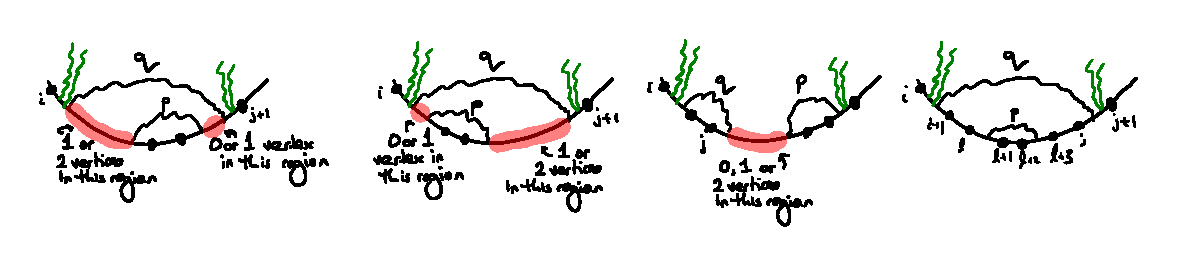
\includegraphics[scale=0.8]{3cases}
    \caption{Four cases for admissible WLDs with no non-supporting vertices. The green half-propagators illustrate where propagators may occur, but are not required to exist; no other regions illustrated may support additional propagators.}\label{fig 3 cases}
  \end{figure}


In each of the four cases, when we remove the propagator labelled $p$ we obtain a diagram which satisfies the statement of the theorem by the induction hypothesis, and contains a propagator ${q = (i,j)}$ with no other propagators inside it (although this region may or may not contain non-supporting vertices, which we will call $l, l+1, \ldots$ as necessary). Let $V$ be the diagram obtained by removing the propagator $p$ from $W$ (Figure \ref{fig V diagram}). 


\begin{figure}
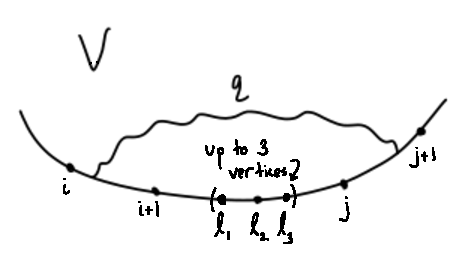
\includegraphics[scale=0.8]{Vdiagram_modified}
\caption{Diagram $V$ is $W$ with $p$ removed; there are no propagators inside $q = (i,j)$, though there may be up to 4 non-supporting vertices labelled $l, l+1, \ldots$.}
\label{fig V diagram}
\end{figure}


Consider the fourth case of Figure~\ref{fig 3 cases} first, as it is the easiest.  In this case, the vertices $\{l,l+1,l+2,l+3 \}$ which support $p$ in $W$ are non-supporting in $V$, so for every propagator $r$ in $V$ (including $q$) we have $J_r^{(V)} = J_r^{(W)}$; these are non-empty cyclic intervals in the correct order by the induction hypothesis.  Additionally, it is clear from Figure~\ref{fig 3 cases} that $J_p^{(W)}(l+a) = \{l+a\}$ for $a\in\{1,2,3\}$ and $J_p^{(W)}(l) = [n] \backslash \{l+1, l+2, l+3\}$. The result therefore holds in this case.


Now we proceed to consider the first three cases of Figure~\ref{fig 3 cases}.
We first describe $J_q^{(V)}(*)$, which can be handled identically for all three cases.

In $V$ there are no propagators inside $q$, so we see from Figure~\ref{fig V diagram} that
\[l, l+1, \ldots ,j \in J^{(V)}_q(j) \text{ (if $l$ exists) and }  j+1 \in J^{(V)}_q(j+1).\]
Note that $j+2 \not\in J^{(V)}_q(j+1)$ by Lemma~\ref{lem no fourth vertex}, so by the induction hypothesis we must have $J^{(V)}_q(j+1) = \{j+1\}$ and $j+2 \in J^{(V)}_q(i)$. Thus there exist vertices $d,e \in [j+2,i+1]$ with $d <e$, such that
\[J^{(V)}_q(i) = [j+2,d-1], \quad J^{(V)}_q(i+1) = [d,e-1], \quad J^{(V)}_q(j) = [e,j], \quad J^{(V)}_q(j+1) = \{j+1\},\]
and all intervals are non-empty.




We now consider what happens as we move from $V$ to each of the three remaining cases for $W$. We need to consider both $J^{(W)}_p$ and $J^{(W)}_r$ for $r \neq p$, since the addition of $p$ can have a knock-on effect on later steps in the algorithm.

%%%%%%%%%

\textbf{Left two cases}: These cases behave essentially identically (except when $j$ or $j+1$ are not in the support of $p$, which can occur in the second case only; see below) so we handle the majority of the proof for these two cases simultaneously. Let $1\leq a\leq 3$ be the number of non-supporting vertices inside $q$ in $V$; so these vertices are $l, \ldots, l+a-1$.  Write $p=(m,m+2)$ where $m\in \{i, i+1, l\}$.  Note that $l, \ldots, l+a-1$ are all in the support of $p$.

We first calculate $I^{(W)}_w$ for a starting vertex ${w \in [n]\backslash \{l, l+1, \ldots,j,j+1\}}$. Note that $p$ has no effect on other propagators for starting vertices in this range, while the value of $I^{(W)}_w(p)$ depends on how soon $q$ is assigned to a vertex, i.e. on the value of $I^{(V)}_w(q)$. Thus, if $w\in J_q^{(V)}(i)$ then
    \[
    I_w^{(W)}(r) =  \begin{cases}
        \max\{i+1, m\} & \text{if } r=p \\
        I_{w}^{(V)}(r) & \text{if } r\neq p
      \end{cases} 
    \]
    while if $w\in J_q^{(V)}(i+1)$ or $w\in J_q^{(V)}(j)$ then
    \[
    I_w^{(W)}(r) =  \begin{cases}
        l & \text{if } r=p \\
        I_{w}^{(V)}(r) & \text{if } r\neq p
      \end{cases} 
      \]
We also need to understand $I^{(W)}_w$ for $w \in \{l,l+1,\ldots,j,j+1\}$. For the majority of these vertices, we use the following observation: if $p$ is the first propagator to be assigned a value by $I_w^{(W)}$, then the remainder of $I_w^{(W)}$ proceeds identically to the assignments of $I^{(V)}_{w+1}$.  Thus we have for any $0\leq b <a$
    \[
    I_{l+b}^{(W)}(r) = \begin{cases}
      l+b & \text{if } r=p\\
      I_{l+b+1}^{(V)}(r) & \text{if } r\neq p
    \end{cases}
    \]
Similarly, if $j$ is in the support of $p$, then we have
     \[
       I_j^{(W)}(r) = \begin{cases}
         j & \text{if $r=p$ and $j$ is in the support of $p$}\\
         I_{j+1}^{(V)}(r) & \text{if $r\neq p$ and $j$ is in the support of $p$}\\
       \end{cases}
       \]
If $j$ is not in the support of $p$, then we must be in the second case of Figure~\ref{fig 3 cases} with two vertices in the right hand region.  In this case, if we start the algorithm at $j$ we need to know whether there will be any unassigned propagators other than $p$ when we reach vertex $i$, so as to know what $p$ contributes.

Consider the WLD $X$ formed from $V$ by moving the second end of $q$ to the edge $j-1$ instead of $j$.  $X$ is still admissible since we have not decreased the support of any set of propagators, so the induction hypothesis applies to it as well.  Note that $J_{j}^{(V)}(r) = J_{j}^{(X)}(r)$ for all $r\neq p$ and $J_{j}^{(X)}(r) = J_{j+1}^{(X)}(r)$ for $r\neq q,p$.  Additionally $I_{j+1}^{(X)}(q) = i$ by the induction hypothesis applied to $X$, and so if we start at $j+1$ and assign propagators to vertices according to the algorithm, when we reach vertex $i$ in $X$ all propagators other than $q$ must have been assigned.  Therefore if we start at $j$ in $W$, we first assign $q$ to $j$ then proceed to assign as in $X$ starting at $j+1$, and hence when we get to $i$ the only remaining unassigned propagator is $p$. Therefore
       \[
       I_j^{(W)}(r) = \begin{cases}

       m & \text{if $r =p$ and $j$ is not in the support of $p$} \\
       I_{j}^{(V)}(r) & \text{if $r\neq p$ and $j$ is not in the support of $p$}\end{cases}
       \] 
Finally, we consider what happens when we start the algorithm at vertex $j+1$. If $j+1$ is in the support of $p$ then we can argue as above to get
\[
       I_{j+1}^{(W)}(r)  = \begin{cases}
         j+1 & \text{if $r=p$ and $j+1$ is in the support of $p$}\\
         I_{j+2}^{(V)}(r) & \text{if $r\neq p$ and $j+1$ is in the support of $p$}.
       \end{cases}
       \]
Now suppose $j+1$ is not in the support of $p$. If we start at $j+1$ we need to know whether there are any unassigned propagators supported on edge $i$ when we reach vertex $i$. We already know that $J_q^{(V)}(j+1) = \{j+1\}$; in particular this means that $q$ contributes $i$ in $I_{j+2}^{(V)}$.  However the construction of $I^{(V)}_{j+1}$ first associates $q$ to $j+1$ and then proceeds identically to $I^{(V)}_{j+2}$.  In particular if $i$ was assigned in $I^{(V)}_{j+1}$, then it would not be available to assign to $q$ in $I^{(V)}_{j+2}$ as all other propagators supported at $i$ in $V$ come before $q$. 

Therefore $p$ is the only potentially unassigned propagator on edge $i$ when we reach vertex $i$ in $W$, and
    \[
    I_{j+1}^{(W)}(r)  = \begin{cases}
      m & \text{if  $r=p$ and $j+1$ is not in the support of $p$}\\
      I_{j+1}^{(V)}(r) & \text{if  $r\neq p$ and $j+1$ is not in the support of $p$}
    \end{cases}
    \]
We can now describe the intervals $J^{(W)}_r(*)$ for the first two cases of Figure~\ref{fig 3 cases}. For $r \neq p$ the intervals are clearly still cyclic and appear in the correct order, and we can assemble the intervals for the $J_p^{(W)}(*)$ as follows.
    \begin{itemize}
      \item 
    If $m=l$ then either $a=2$ (so $l+1=m+1$, $j=m+2$, and $j+1=m+3$) or $a=3$ (so $l+1=m+1$, $l+2=m+2$, $j=m+3$, and $j+1$ is not in the support of $p$), and in both cases
    \begin{gather*}
    J^{(W)}_p(m) = [m+4, m], \qquad  J^{(W)}_p(m+1) = \{m+1\}, \\ J^{(W)}_p(m+2) = \{m+2\}, \qquad  J^{(W)}_p(m+3) = \{m+3\},
    \end{gather*}
    which are nonempty and otherwise as required.
  \item
        If $m=i+1$ then checking each of the three different possibilities for $a$ we likewise get
    \begin{gather*}
    J^{(W)}_p(m) = [m+4, d-1], \qquad  J^{(W)}_p(m+1) = [d, m+1], \\  J^{(W)}_p(m+2) = \{m+2\}, \qquad  J^{(W)}_p(m+3) = \{m+3\},
    \end{gather*}
    which are nonempty and otherwise as required.
  \item If $m=i$ then $a=1$ or $a=2$, in the former case $l=m+2$, $j=m+3$ and $j+1$ is not in the support of $p$ so
    \begin{gather*}
    J^{(W)}_p(m) = \{m+4\}, \qquad  J^{(W)}_p(m+1) = [m+5, d-1], \\  J^{(W)}_p(m+2) = [d, m+2], \qquad  J^{(W)}_p(m+3) = \{m+3\},
    \end{gather*}
    while in the latter $l=m+2$, $l+1=m+3$, and $j$ and $j+1$ are not in the support of $p$ so
    \begin{gather*}
    J^{(W)}_p(m) = [m+4, j+1], \qquad  J^{(W)}_p(m+1) = [j+2, d-1], \\  J^{(W)}_p(m+2) = [d, m+2], \qquad  J^{(W)}_p(m+3) = \{m+3\},
    \end{gather*}
    which are again as required.
    \end{itemize}

\textbf{Third case}: In this case there are no non-supporting vertices $l, l+1, \ldots$ inside $q$.  Again write $p=(m, m+2)$ where $m\in \{j, j+1, j+2\}$. We proceed as in the previous cases, by computing $I^{(W)}_w$ for vertices $w$ in roughly increasing order of difficulty.

For $w \in [n]\backslash\{j+1,m,m+1,m+2,m+3\}$: if $w\in J_q^{(V)}(i)$ or $w\in J_q^{(V)}(i+1)$ then
    \[
    I_w^{(W)}(r) =  \begin{cases}
        m & \text{if } r=p \\
        I_{w}^{(V)}(r) & \text{if } r\neq p
      \end{cases} 
    \]
    while if $w\in J_q^{(V)}(j)$ then
    \[
    I_w^{(W)}(r) =  \begin{cases}
        \max\{m, j+1\} & \text{if } r=p \\
        I_{w}^{(V)}(r) & \text{if } r\neq p
      \end{cases} 
    \]

Finally, for $j+1$ and the vertices in the support of $p$, we have

\begin{align*}
  I_{j+1}^{(W)}(r) &= \begin{cases}
    j+1 & \text{if } r=q\\
    j+2 & \text{if } r=p\\
    I_{j+3}^{(V)}(r) & \text{if } r\neq p,q
  \end{cases}\\
  I_m^{(W)}(r) &= \begin{cases}
    m & \text{if $r=p$ and $q$ not supported on $m$}\\
    m+1 & \text{if $r=p$ and $q$ supported on $m$}\\
    I_{m}^{(V)}(r) & \text{if } r\neq p
  \end{cases}\\
  I_{m+1}^{(W)}(r) & = \begin{cases}
    m+1 & \text{if $r=p$ and $q$ not supported on $m+1$} \\
    m+2 & \text{if $r=p$ and $q$ supported on $m+1$} \\
    I_{m+1}^{(V)}(r) & \text{if } r\neq p,q
  \end{cases}\\
  I_{m+2}^{(W)}(r) & = \begin{cases}
    m+2 & \text{if } r=p \\
    I_{m+3}^{(V)}(r) & \text{if } r\neq p
  \end{cases}\\
  I_{m+3}^{(W)}(r) & = \begin{cases}
    m+3 & \text{if } r=p \\
    I_{m+4}^{(V)}(r) & \text{if } r\neq p
  \end{cases}
\end{align*}
Note that $I_{m+2}^{(V)}(r) = I_{m+3}^{(V)}(r)$ for all propagators $r$ in $V$, and that if $j+1\not\in\{m, m+1, m+2, m+3\}$ then $j+2$ and $j+3$ are non-supporting vertices in $V$, so in that case $I_{j+2}^{(V)}(r) = I_{j+3}^{(V)}(r) = I_{j+4}^{(V)}(r)$ for $r$ in $V$. 

Therefore, once again we can see that the $J_r^{(W)}(*)$ are cyclic for all $r\neq p$ in $W$.  Assembling the intervals for $p$ we have:
\begin{itemize}
\item if $m=j$ then
\begin{gather*}J_p^{(W)}(m) = [m+4,e-1], \qquad  J_p^{(W)}(m+1) = [e,m], \\  J_p^{(W)}(m+2) = [m+1,m+2], \qquad  J_p^{(W)}(m+3) = \{m+3\},\end{gather*}
\item if $m=j+1$ then
\begin{gather*}J_p^{(W)}(m) = [m+4,m-1], \qquad J_p^{(W)}(m+1) = [m,m+1], \\  J_p^{(W)}(m+2) = \{m+2\}, \qquad  J_p^{(W)}(m+3) = \{m+3\},\end{gather*}
\item if $m=j+2$ then
\begin{gather*}J_p^{(W)}(m) = [m+4,m], \qquad  J_p^{(W)}(m+1) = \{m+1\}, \\  J_p^{(W)}(m+2) = \{m+2\}, \qquad  J_p^{(W)}(m+3) = \{m+3\}.\end{gather*}
\end{itemize}
The result now follows by induction.
\end{proof}



We need one more lemma before we can prove that Algorithm~\ref{alg:put GN on WLD} does in fact give the Grassmann necklace of the positroid associated to $W$.

\begin{lem}\label{lem basis as perm}
Let $W = (\cP,[n])$ be an admissible Wilson loop diagram and let $M(W)$ be its associated matroid. A subset $J \subseteq [n]$ is an independent set of $M(W)$ if and only if there exists an injective set map $f : J \rightarrow \cP$ with the property that for each $j\in J$ we have $j \in V(f(j))$.
\end{lem}

One of the most important uses of this lemma is for bases.  The lemma says that a subset $J$ of $[n]$ is a basis of $M(W)$ if and only if there is a set bijection between $J$ and $\cP$ with the property that for each $j\in J$ the propagator associated to $j$ under the bijection is supported on vertex $j$.

\begin{proof}
Because the nonzero entries of $C(W)$ are independent indeterminants, $J$ is an independent set is if and only if there is some choice of $|J|$ nonzero entries of $C(W)$ one in each row associated to an element of $J$ and each in different columns.

Each entry in $C(W)$ identifies a propagator by the row of the entry and a vertex by the column of the entry.  The entry is nonzero if and only if the propagator is supported on that vertex.

Consequently, a choice of $|J|$ nonzero entries of $C(W)$ one in each row associated to an element of $J$ and each in different columns is equivalent to an assignment of the propagators of $J$ to supporting vertices so that no two are assigned to the same vertex.  Such an assignment of the propagators of $J$ to supporting vertices is exactly a map $f$ as described in the statment, hence proving the result.
\end{proof}

\begin{thm}\label{res:alg gives GN}
The sequence of $k$-subsets $(I_1,\dots,I_n)$ obtained by applying Algorithm~\ref{alg:put GN on WLD} to all vertices of an admissible diagram $W$ is exactly the Grassmann necklace of $M(W)$.
\end{thm}

\begin{proof}
For each $i \in [n]$, let $I_i$ be the set of vertices assigned to the propagators of $W$ by Algorithm~\ref{alg:put GN on WLD} with starting vertex $i$. By Lemma~\ref{GN alg well defined}, we know that $|I_i| = k$ for each $i \in [n]$. By [ref], the sequence $(I_1, \dots, I_n)$ is a Grassmann necklace if and only if $I_{i+1} \supseteq I_i \backslash \{i\}$ for all $i \in [n]$.


Suppose for a contradition that there exists an admissible diagram for which there exists an $i$ with $k\in I_{i\backslash\{i\}}$ and $k \not\in I_{i+1}$.  Fix $n$.  Let the triple $(W, i, k)$ be such a counterexample on $n$ vertices which is minimal with respect to the number of propagators. %, and among all those counterexamples on $n$ vertices with the same number of propagators, let $(W,i,k)$ be minimal with respect to the distance from $i$ to $k$ in the $\leq _i$ order.

If $i \not\in I_i$, then there are no propagators supported on $i$ at all.  In this case it is clear that applying Algorithm~\ref{alg:put GN on WLD} at vertex $i$ and vertex $i+1$ produces exactly the same result, i.e. $I_{i+1} = I_i$, and so $(W, i, k)$ is not a counterexample at all.

Now suppose that $i \in I_i$.  Let $p$ be the propagator which contributes $i$ to $I_i$; thus one end of $p$ must lie on either edge $i-1$ or edge $i$.  In both cases let $b$ denote the edge supporting the other end of $p$.

\textbf{Case I}:  Suppose $p$ has one end on edge $i-1$.  Then $p$ is not supported on $i+1$, so in building $I_{i+1}$ we will take the same propagators as in the construction of $I_i$ from vertices $i+1$ up to $b-1$, that is $I_{i+1} \cap [i+1,b-1] = I_{i} \cap [i+1,b-1]$.  Furthermore, by Lemma~\ref{vertex cyclic int lem}, when building $I_{i+1}$ it must happen that $p$ is taken at vertex $b$, as otherwise $b$ would never be contributed by $p$.    Consequently, in building $I_{i+1}$, when the algorithm reaches vertex $b$ there cannot be any unassigned propagators remaining that are before $p$.  This is also true in when the algorithm constructing $I_i$ reaches $b$, since the same propagators have been assigned beforehand.  Finally, we also note that $k\geq_i b+1$.

Let $W'$ be the diagram obtained from $W$ by removing both $p$ and all propagators inside of $p$ (recall Definition~\ref{props inside p}).

By the above observations, if we commence Algorithm~\ref{alg:put GN on WLD} in $W'$ from vertex $b$, then we are in the same situation with respect to unassigned propagators as if we began at $i$ in $W$ and proceeded to $b$ following the algorithm; the propagators we assigned in the latter case are exactly the ones removed to build $W'$.  Similarly, starting at $i+1$ in $W$ and moving to $b+1$ leaves us in the same situation with respect to unassigned propagators as beginning at $b+1$ in $W'$ would.  This gives the equations
\begin{align*}
  I_i^{(W)} \cap [b,i-1] & = I_b^{(W')} \\
  I_{i+1}^{(W)} \cap [b+1,i-1] & = I_{b+1}^{(W')}
\end{align*}
where the diagram is indicated in the superscript.
Thus we have $k\in I_b^{(W')}\setminus\{b\}$ and $k\not\in I_{b+1}^{(W')}$, contradicting the minimality of $(W, i, k)$.

\textbf{Case II}: Suppose $p$ has one end on edge $i$.  Note that by assumption we have $I_i(p) = i$; this means that $p$ must be the first propagator lying on edge $i$, and hence we must have $I_{i+1}(p) = i+1$ as well.  Observe also that $k\geq_i i+2$ since $i+1\in I_{i+1}$.

Let $W'$ be the diagram obtained from $W$ by removing only the propagator $p$.  Then we have
\begin{align*}
  I_i^{(W)} \backslash \{i\} & = I_{i+1}^{(W')} \\
  I_{i+1}^{(W)} \backslash \{i+1\} & = I_{i+2}^{(W')}
\end{align*}
since in both cases the algorithm in $W'$ proceeds identically to that in $W$ after assigning $p$. Since $k \neq i+1$, we have $k\in I_{i+1}^{(W')}\setminus\{i+1\}$ but $k\not\in I_{i+2}^{(W')}$, contradicting the minimiality of $(W, i, k)$.

%If $i \not\in I_i$, then there are no propagators supported on $i$ at all.  In this case it is clear that applying Algorithm~\ref{alg:put GN on WLD} at vertex $i$ and vertex $i+1$ produces exactly the same result, i.e. $I_{i+1} = I_i$.
%
%Now suppose that $i \in I_i$.  Order $I_i$ and $I_{i+1}$ with respect to $\leq_{i+1}$; in particular, $i$ is the last term in $I_i$ with respect to this ordering.
%
%Let $p_1$ be the rightmost propagator supported on $i$, and suppose it is removed at step $a$ with respect to vertex $i+1$.  This is the first point at which $I_{i+1}$ can differ from $I_i$, i.e. we have $I_{i+1} \cap \interval{i+1}{a-1} = I_{i} \cap \interval{i+1}{a-1}$.  If $a \not\in I_i$, then $p_1$ is the only propagator supported on $a$ at step $a$ with respect to vertex $i+1$.  All remaining steps are unchanged and we conclude that $I_{i+1} = I_i \backslash \{i\} \cup \{a\}$.
%
%If $a \in I_i$, then at step $a$ with respect to vertex $i+1$ there must be another propagator $p_2$ which lies to the left of $p_1$.  We have $I_{i+1} \cap \interval{i+1}{a} = I_i \cap \interval{i+1}{a}$, and the next possible difference
%
%{\color{red}[argh]}
%
%Although there are many different subcases to consider, the idea is always the same: we look for the first entry where $I_{i+1}$ and $I_i \backslash \{i\}$ differ (with respect to $<_{i+1}$), and show that this is the only possible difference.
%
%The reader should keep in mind that due to Proposition~\ref{res:alg k labels}, the following process cannot double back on itself.
%
%\begin{enumerate}
%\item If $p_1$ contributes $k$ to $I_{i+1}$ and $k \in I_i$, then there is another propagator $p_2$ which was deleted at step $k$ with respect to vertex $i$, but now survives at step $k$ with respect to vertex $i+1$.  All intermediate steps of the algorithm are unchanged, so $I_{i+1}$ and $I_i \backslash \{i\}$ agree up to (and including) $k$.
%\item We now look at which label $p_2$ contributes in $I_{i+1}$, and apply the same argument.  Iterate this process until we find a propagator $p_r$ which is deleted at step $j$ with respect to vertex $i+1$, but $j \not\in I_i$.
%\item $j \not\in I_i$ implies that $p_r$ is the \textit{only} propagator supported on vertex $j$ at this step.  There is therefore no knock-on effect, and any remaining propagators in the diagram contribute the same label to both $I_i$ and $I_{i+1}$. We conclude that $I_{i+1} = I_i \backslash \{i\} \cup \{j\}$.
%\end{enumerate}

\medskip

We have shown that $(I_1,\dots,I_n)$ is a Grassmann necklace; it remains to check that this Grassmann necklace corresponds to the positroid $M(W)$.  We need to show that:
\begin{itemize}
\item For each $i \in [n]$, $I_i$ is a basis for $M(W)$.
\item If $J$ is lexicographically smaller than $I_i$ with respect to $<_i$, then $J$ is not a basis for $M(W)$.\note{Si\^an note to self: check whether it's lex smaller or Gale smaller}
\end{itemize}
The algorithm is pairing each $j \in I_i$ with a unique propagator supported on that vertex so by Lemma~\ref{lem basis as perm} $I_i$ is a basis for $M(W)$.
%%Recall from [ref] that a $k$-subset $J \in \binom{[n]}{k}$ is a basis for $\PP_W$ if and only if it has no subset $U \subseteq J$ such that $|U| > |Prop(U)|$.  It is immediately clear from the construction that $I_i$ is a basis for each $i$: the algorithm is pairing each $j \in I_i$ with a unique propagator supported on that vertex, so $|Prop(U)| \geq U$ for all $U \subseteq I_i$.

%%If $\exists l \in J$ with $Prop(l) = \emptyset$ then $J$ is clearly not a basis, so suppose otherwise.  Write
%%\[I_i = [i_1 <_i i_2 <_i \dots <_i i_r <_i \dots <_i i_k], \quad J = [i_1 <_i i_2 <_i \dots <_i j_r <_i \dots <_i j_k],\]
%%so that $I_i$ and $J$ differ for the first time in the $r$th position.  Then
%%\[r-1 \geq |Prop(\{i_1, \dots, i_{r-1}\})| = |Prop(\{i_1, \dots, i_{r+1},j_r\})|,\]
%%If $|Prop(\{i_1, \dots, i_{r-1}|\}| = r-1$ then we are done; otherwise

Suppose we have a $k$-set $J$ such that $J$ is a basis for $M(W)$ and yet is lexicographically less than $I_i$ with respect to $<_i$.  By Lemma~\ref{lem basis as perm} there is a set bijection between $J$ and the propagators of $W$ such that for each $j \in J$, the propagator associated to $j$ is supported on vertex $j$.  Choose one such bijection.  For a propagator $p$ of $W$ write $J(p)$ for the associated $j$ according to this bijection.

Since $J$ is lexicographically smaller than $I_i$, the $<_i$-smallest element of the symmetric difference of $J$ and $I_i$ is some $j_0\in J$, $j_0 \not\in I_i$. Let $p_1$ be the propagator such that $J(p_1)=j_0$.  Since $j_0\not\in I_i$ but $p_1$ is supported at $j_0$, then $p_1$ must have been assigned to an earlier vertex by $I_i$, i.e. we have $I_i(p_1) <_i j_0$.  Let $j_1 = I_i(p_1)$.

However, $j_0$ is the $<_i$-smallest element in the symmetric difference of $J$ and $I_i$, so in particular there is some propagator $p_2$ such that $J(p_2)=I_i(p_1)$.  Now, let $j_2 = I_i(p_2)$ and note that $j_2 \neq J(p_2)$ (since $I_i(p_1)=J(p_2)$), so either $I_i(p_2) \not\in J$ or there is a propagator $p_3$ such that $J(p_3) = I_i(p_2)$.  Continuing likewise we get a list of vertices $j_k$ and propagators $p_k$ such that $J(p_k) = I_i(p_{k-1}) = j_{k-1}$.

We claim that the propagators and vertices in this list are distinct.  The claim is proved by induction.  The definition of $j_0$ gives that $j_0$ and $j_1$ are distinct and that $p_1$ and $p_2$ are distinct.  Now, suppose we have $p_k$ and $j_k$ with $I_i(p_k)=j_k$ and with $j_k\in J$.  Then $p_{k+1}$ is the propagator associated to $j_k$ by the fixed bijection we have chosed for $J$.  Since $j_k$ is distinct from the previous $j_j$, $p_{k+1}$ is distinct from the previous $p_j$.  Then $j_{k+1} = I_i(p_{k+1})$, but $I_i$ is also a bijection, so since $p_{k+1}$ is distinct from the other $p_j$ we have that $j_{k+1}$ is distinct from the other $j_j$ for $1\leq j\leq k$.  Additionally $j_{k+1}\neq j_0$ since $j_0\not\in I_i$ but $j_{k+1}\in I_i$.  This proves the claim.

By finiteness the list must end, and the only way it can end is with some $p_k$ such that $j_k = I_i(p_k)\not\in J$, so in particular $j_k >_i j_0$.  

Next we will prove that $j_k <_i j_0$ for all $k > 0$.  This gives a contradiction to the exisitence of $J$ and completes the proof of the theorem.  This proof will also be by induction, however, for the induction to go through nicely we will need to prove the following slightly stronger statement:
for all $k>0$ in the list
\begin{itemize}
\item $j_k <_i j_0$ and
\item either
  \begin{itemize}
  \item $I_i(p_k) <_i J(p_k)$, or
  \item there exists an $ell<k$ such that $I_i(p_\ell) <_i J(p_\ell)$, those two vertices are supported by distinct ends of $p_\ell$ and $p_k$ is on the side of $p_l$ which runs from $I_i(p_\ell)$ to $J(p_\ell)$.
  \end{itemize}
\end{itemize}


We already observed that $j_1 <_i j_0$ and $I_i(p_1) <_k J(p_1)$ so we have the base case for the induction.  Suppose we have the inductive hypothesis for all indices less than $k>1$ and that $p_k$ exists.

By definition $J(p_k) = I_i(p_{k-1}) = j_{k-1}$, so $p_{k-1}$ and $p_{k}$ are both supported at $j_{k-1}$, but $I_{i}(p_{k-1}) = j_{k-1}$.  Thus either $p_{k-1}$ appears before $p_k$ in the neighbourhood of $j_{k-1}$ or $p_k$ was taken earlier by $I_i$ so $I_i(p_k) <_i I_i(p_{k-1})$.  In the latter case we are done as $j_k = I_i(p_k) <_i j_{k-1} <_i j_0$ which is what we want.  So we now assume that $p_{k-1}$ appears before $p_k$ in the neighbourhood of $j_{k-1}$.

If $I_i(p_{k-1}) <_i J(p_{k-1})$ and these are vertices supported by distinct ends of $p_{k-1}$ then $p_{k}$ coming after $p_{k-1}$ around $j_{k-1}$ implies that $p_k$ is on the $I_i(p_{k-1})$ to $J(p_{k-1})$ side of $p_{k-1}$.  Therefore $j_k = I_i(p_k) \leq_i J(P_{k-1}) + 1$.  If $k-1 \neq 1$ then this gives $j_k \leq_i I_i(p_{k-2}) + 1 <_i j_0$ so $j_k \leq_i j_0$, but $j_0\not\in I_i$ so $j_k<_i j_0$.  If $k-1= 1$ then either $j_k <_i j_0$ or we have the configuration
\[
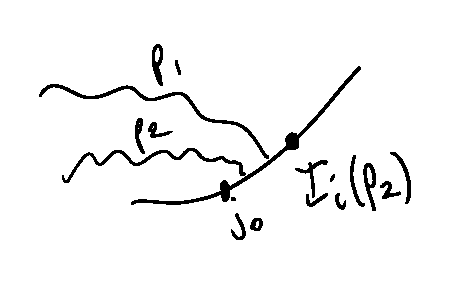
\includegraphics{impossible_config}
\]
which is impossible as $p_2$ is supported at $j_0$ but not taken in $I_i$ until after $j_0$ even though $j_0\not\in I_i$.  Taking all of this paragraph together we are done unless $I_i(p_{k-1})\not<_i J(p_{k-1})$ so now assume this.

By the induction hypothesis,  $I_i(p_{k-1})\not<_i J(p_{k-1})$ implies that there exists and $\ell < k-1$ such that $p_{k-1}$ is on the side of $p_{\ell}$ that goes from $I_i(p_\ell)$ to $J(p_\ell)$.  If $j_{k-1}$ is not in the support of the $J(p_\ell)$ end of $p_\ell$ then $p_{k-1}$ before $p_{k}$ around $j_{k-1}$ implies that $p_k$ is on the same side of $p_\ell$ as $p_{k-1}$ is.  Then the same arguments as above with $\ell$ in place of $k-1$ give $j_k \leq_i J(P_\ell)+1$ implying $j_k <_i j_0$ which is everything we need.

It remains to consider when $j_{k-1}$ is in the support of the $J(p_\ell)$ end of $p_\ell$, call this case $(*)$.  Since $J(p_\ell) = j_{\ell-1}$ and the $j_i$ are distinct this means that we have one of the following two configurations
\[
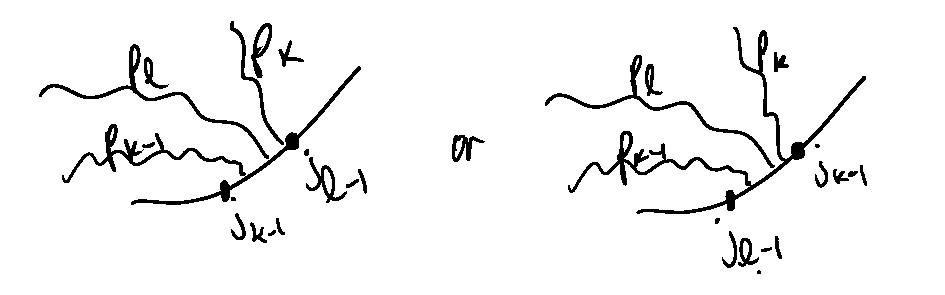
\includegraphics{induction_conf}
\]
If $p_\ell=p_1$ then $j_{\ell-1}=j_0$ and then as $j_0\not\in I_i$ but $p_k$ is supported at $j_0$ we get $I_i(p_k) <_i j_0$ and also $I_i(p_k) <_i j_{k-1} = J(p_k)$ as the only vertices not yet taken for $I_i(p_k)$ must be before both labelled vertices in the illustration.

If $p_\ell \neq p_1$ then we argue as above with $\ell-1$ in place of $k-1$: in particular $J(p_\ell) = I_i(p_{\ell-1})$ but $p_k$ is supported at $p_{\ell-1}$, so either $I_i(p_k) <_i I_i(p_{\ell-1})$ in which case as before we get desired conclusion, or $p_k$ comes before $p_{\ell-1}$ at $j_{\ell-1}$.  Then again argue as before getting a new $p_{\ell'}$ in place of $p_{\ell}$, except that then case $(*)$ must occur simultaneously for both $p_{\ell'}$ and $p_{\ell}$ with respect to $p_{k}$.  This can only occur if $j_{\ell-1}, j_{k-1}, j_{\ell'-1}$ are consecutive.  Iterating the argument one more time we finally cannot have case $(*)$ as then all neighbouring vertices of $j_{k-1}$ are used up.

This completes the induction and thence the proof of the theorem.

%Since $J$ is lexicographically smaller than $I_i$, the $<_i$-smallest element of the symmetric difference of $J$ and $I_i$ is some $j_0\in J$, $j_0 \not\in I_i$. Let $p$ be the propagator such that $J(p)=j_0$.  Since $j_0\not\in I_i$ but $p$ is supported at $j_0$, then $p$ must have been assigned to an earlier vertex by $I_i$, i.e. we have $I_i(p) <_i j_0$.  Thus the propagator $p$ has the following property, which we call property $A$:
%\begin{equation}\label{propertyA}\tag{A}I_i(p) <_i J(p) \text{ \ and \ }I_i\cap [i,I_i(p)] = J\cap [i,I_i(p)]. \end{equation}
%
%{}From the previous paragraph we conclude that if we ever had a $J$ which is lexicographically less than $I_i$ and yet a basis of $M(W)$, then there exists a propagator $p$ which has property $A$.
%
%Finally, we will prove that whenever there is a propagator $p$ which has property $A$ then there is another propagator $r$ which also has property $A$ and for which $I_i(r) <_i I_i(p)$.  This would lead to an infinte regress, contradicting the finiteness of $I_i$; thus there could be no such $J$, which will complete the proof of the proposition.
%
%So suppose $p$ has property $A$.  The same vertices in $[i,I_i(p)]$ are in the image of the assignment from $J$ and the image of the assignment from $I_i$ so the same number of propagators are assigned to vertices in this interval by each assignment.  However $p$ is one of the propagators assigned to a vertex in this interval in $I_i$ but not in $J$.  Thus there exists a propagator $q$ for which $J(q)\in [i,I_i(p)]$ but $I_i(q) >_i I_i(p)$.  Therefore $J(q)<_i I_i(q)$ and  $I_i\cap [i,J(q)] = J\cap [i,J(q)]$.  This is analogous to property $A$ but with the roles of $J$ and $I_i$ switched.  Thus by the same argument we must have a propagator $r$ for which $I_i(r)\in[i,J(q)]$ but $J(r)>_i J(q)$.  It follows that $r$ also has property $A$ and that
%\[I_i(r) \leq_i J(q) \leq_i I_i(p)\]
%\hlfix{as required.}{We need $I_i(r) <_i I_i(p)$ but I'm having trouble seeing it?}
\end{proof}





In an arbitrary Grassmann necklace, it is possible for an index $i$ to appear in no terms of the Grassmann necklace (a {\em loop}) or in all terms of the necklace (a {\em coloop}). Using Theorem~\ref{res:alg gives GN}, a characterization of the loops and coloops of the Grassmann necklace associated to a Wilson loop diagram follows easily.


\begin{cor}\label{no coloops}
Grassmann necklaces coming from admissible Wilson loop diagrams have no coloops. A vertex $j$ is a loop if and only if $j$ supports no propagators. 
\end{cor}
\begin{proof}
For any $i \in [n]$, $i-1$ is maximal with respect to the $<_{i}$ order. Therefore there can be no propagator $p$ with $I_{i}(p) = i-1$ by Lemma~\ref{lem no fourth vertex}, i.e. $i-1 \not\in I_{i}$. Thus the Grassmann necklace admis no coloops.

If $j \in [n]$ is a loop then $j \not\in I_j$, which can only happen if there are no propagators supported on vertex $j$. Conversely, if $j$ supports no propagators, then Algorithm~\ref{alg:put GN on WLD} never assigns a propagator to $j$ and hence $j \not\in I_i$ for all $i \in [n]$.
\end{proof}





\subsection{Dimension of the Wilson Loop cells}

Our next goal is to show that the dimension of the positroid cell defined by a Wilson loop diagram $(\cP, [n])$ has dimension $3|\cP|$.  Marcott in ***cite this*** has a different proof which is geometric and more elegant, but it is not easy to track the effect of a particular propagator.  Our approach is much more explicit.


Recall that the dimension of a positroid cell is equal to the number of plusses in the associated Le diagram \cite[Theorem 6.5]{Postnikov}. By combining Algorithms~\ref{alg:put GN on WLD} and \ref{alg:GN to Le} (converting from WLD to Grassmann necklace to Le diagram) we explicitly describe the effect of adding another propagator to a Wilson loop diagram in terms of the plusses of the associated Le diagrams, and hence give a recursive proof of the $3|\cP|$-dimensionality of the cells.

We start with several lemmas, of roughly increasing degree of technicality.

\begin{lem}\label{lem uncovered}

Let $W$ be an admissible Wilson loop diagram with $k$ propagators, and with a vertex $i$ that supports no propagators.  Let $V$ be $W$ with vertex $i$ removed.  Then the Le diagram of $W$ is obtained from the Le diagram of $V$ by inserting an extra column containing all $0$s in position $i$ (i.e. such that the new column has the label $i$).
\end{lem}

\begin{proof}
  By Algorithm~\ref{alg:put GN on WLD} the Grassmann necklace of $W$ is obtained from the Grassmann necklace of $V$ by duplicating the $i$th element of the Grassmann necklace of $V$ (shifting indices as appropriate), and incrementing all indices greater than $i$ in each Grassmann necklace element.  Formally, if $I_1^{V}, \ldots, I_{n-1}^{V}$ and $I_1^{W}, \ldots, I_n^{W}$ are the Grassmann necklaces of $V$ and $W$ respectively then
  \[
  I_j^{W} =
  \begin{cases}
    \{\ell \in I_j^{V} : \ell < i\} \cup \{\ell+1 \in I_j^{V} : \ell \geq i\} & \text{if $j\leq i$} \\
    \{\ell \in I_{j-1}^{V} : \ell < i\} \cup \{\ell+1 \in I_{j-1}^{V} : \ell \geq i\} & \text{if $j > i$.}
  \end{cases}
  \]


By Lemma~\ref{no coloops} we know that $i \not\in I_1^W$, and so $i$ must label a horizontal edge on the boundary of the Le diagram of $W$, i.e. it must be a column label. The shapes of the Le diagram of $V$ and $W$ are the same except for the insertion of this column since $I_1^*$ is the same for $V$ and $W$ except for the incrementation of the indices $\geq i$ in the transition from the necklace for $V$ to the necklace for $W$. 
\end{proof}


\begin{lem}\label{lem dihedral}
If two Wilson loop diagrams differ by a dihedral transformation then their Le diagrams have same number of plusses.
\end{lem}
\begin{proof}
By \cite[Proposition 17.10]{Postnikov}, the dimension of a positroid (and hence the number of plusses in its Le diagram) is $k(n-k) - A(\pi_W)$, where $A(\pi_W)$ denotes the number of alignments of the decorated permutation $\pi_W$ of the positroid associated to $W$. (See \cite[Figure 17.1]{Postnikov} and preceding discussion.)

It can easily be seen from \cite[Section 17]{Postnikov} and Algorithm \ref{alg:put GN on WLD} that dihedral transformations of a Wilson loop diagram $W$ correspond to dihedral transformations of the chord diagram representation of $\pi_W$. Since the number of alignments in a chord diagram is preserved under dihedral transformations, the result follows.
\end{proof}


\begin{lem}\label{lem good p}
  Let $W$ be an admissible Wilson loop diagram with $n\geq 1$ propagators.  Then there is some dihedral transformation $W'$ of $W$ such that $W'$ has a propagator $p$ with the following properties.
  \begin{itemize}
  \item $p = (i, n-1)$ for some $i$, and $p$ has no propagators inside it (that is $i+2, \ldots, n-2$ do not support any propagators in $W'$).
  \item Either the edge $i$ in $W'$ only supports $p$ or the edge $i$ in $W'$ supports exactly one other propagator $q = (j, i)$ with no other propagators inside $q$.
  \end{itemize}
\end{lem}

\begin{proof}
  Remove all vertices of $W$ which do not support any propagators to get a weakly admissible Wilson loop diagram $V$.  Lemma~\ref{lem sian} applied to $V$ gives a length 2 propagator $p$ in $V$ for which either no other propagator is supported on one of the supporting edges of $p$ or there is a second length 2 propagator which is the only other propagator supported on one of the supporting edges of $p$.  (Figure~\ref{fig 3 cases} shows the possible configurations arising from Lemma~\ref{lem sian}, and the reader can easily check that in each case $p$ must be in one of the two situations described above.)

  We can now make a dihedral transformation of $V$ to obtain a diagram satisfying the statement of the lemma with $p$ and $q$ both length 2. Restoring the vertices which do not support any propagators, we obtain a dihedral transformation $W'$ of $W$ as desired (with potentially longer lengths for $p$ and $q$).
\end{proof}



Combining Lemmas \ref{lem uncovered}, \ref{lem dihedral}, and \ref{lem good p}, it therefore suffices to study the Le diagrams of weakly admissible Wilson loop diagrams admitting one of the configurations described in Lemma~\ref{lem good p} with propagators $p$ and $q$ (if $q$ exists) both of length 2. See Figure~\ref{fig special p} for an illustration of the two possibilities.

The next few lemmas describe how diagrams of this type are related to the corresponding diagram with propagator $p$ removed, first in terms of the Grassmann necklaces and then in terms of the Le diagrams. These technical lemmas will form the backbone of the inductive step in the main dimensionality argument.

\begin{lem}\label{lem I}
Let $W$ be an admissible Wilson loop diagram with $n\geq 1$ propagators, and suppose that $W$ admits one of the configurations described in Lemma~\ref{lem good p}, with $p$ and $q$ (if $q$ exists) both of length 2. Let $V$ be $W$ with $p$ removed.  Then

  \begin{align*}
    I_1^{W} & = I_1^{V} \cup \{n-3\} \\
    I_n^{W} & = I_1^{V} \cup \{n\} \\
    I_{n-1}^{W} & = I_n^{V} \cup \{n-1\} \\
    I_{n-2}^{W} & =
    \begin{cases}
      I_{n-2}^{V}\cup \{n-2\} & \text{if $n-2\not\in I_{n-2}^{V}$} \\
      I_{n-2}^{V}\cup \{n-1\} & \text{if $n-2\in I_{n-2}^{V}$, $n-1\not\in I_{n-2}^{V}$} \\
      (I_{n}^{V} - \{n-5\})\cup \{n-1,n-2\} & \text{if $n-1, n-2\in I_{n-2}^{V}$}
    \end{cases} \\
    I_{k}^{W} & =
    \begin{cases}
      I_k^{V}\cup \{n-3\} & \qquad \qquad \qquad \qquad \text{if $n-3 \not\in I_k^{V}$}\\
      I_k^{V}\cup\{n-2\} & \qquad \qquad \qquad \qquad \text{if $n-3\in I_k^{V}$}
    \end{cases} \\
    & \text{for $1<k<n-2$}
  \end{align*}
\end{lem}

\begin{figure}
 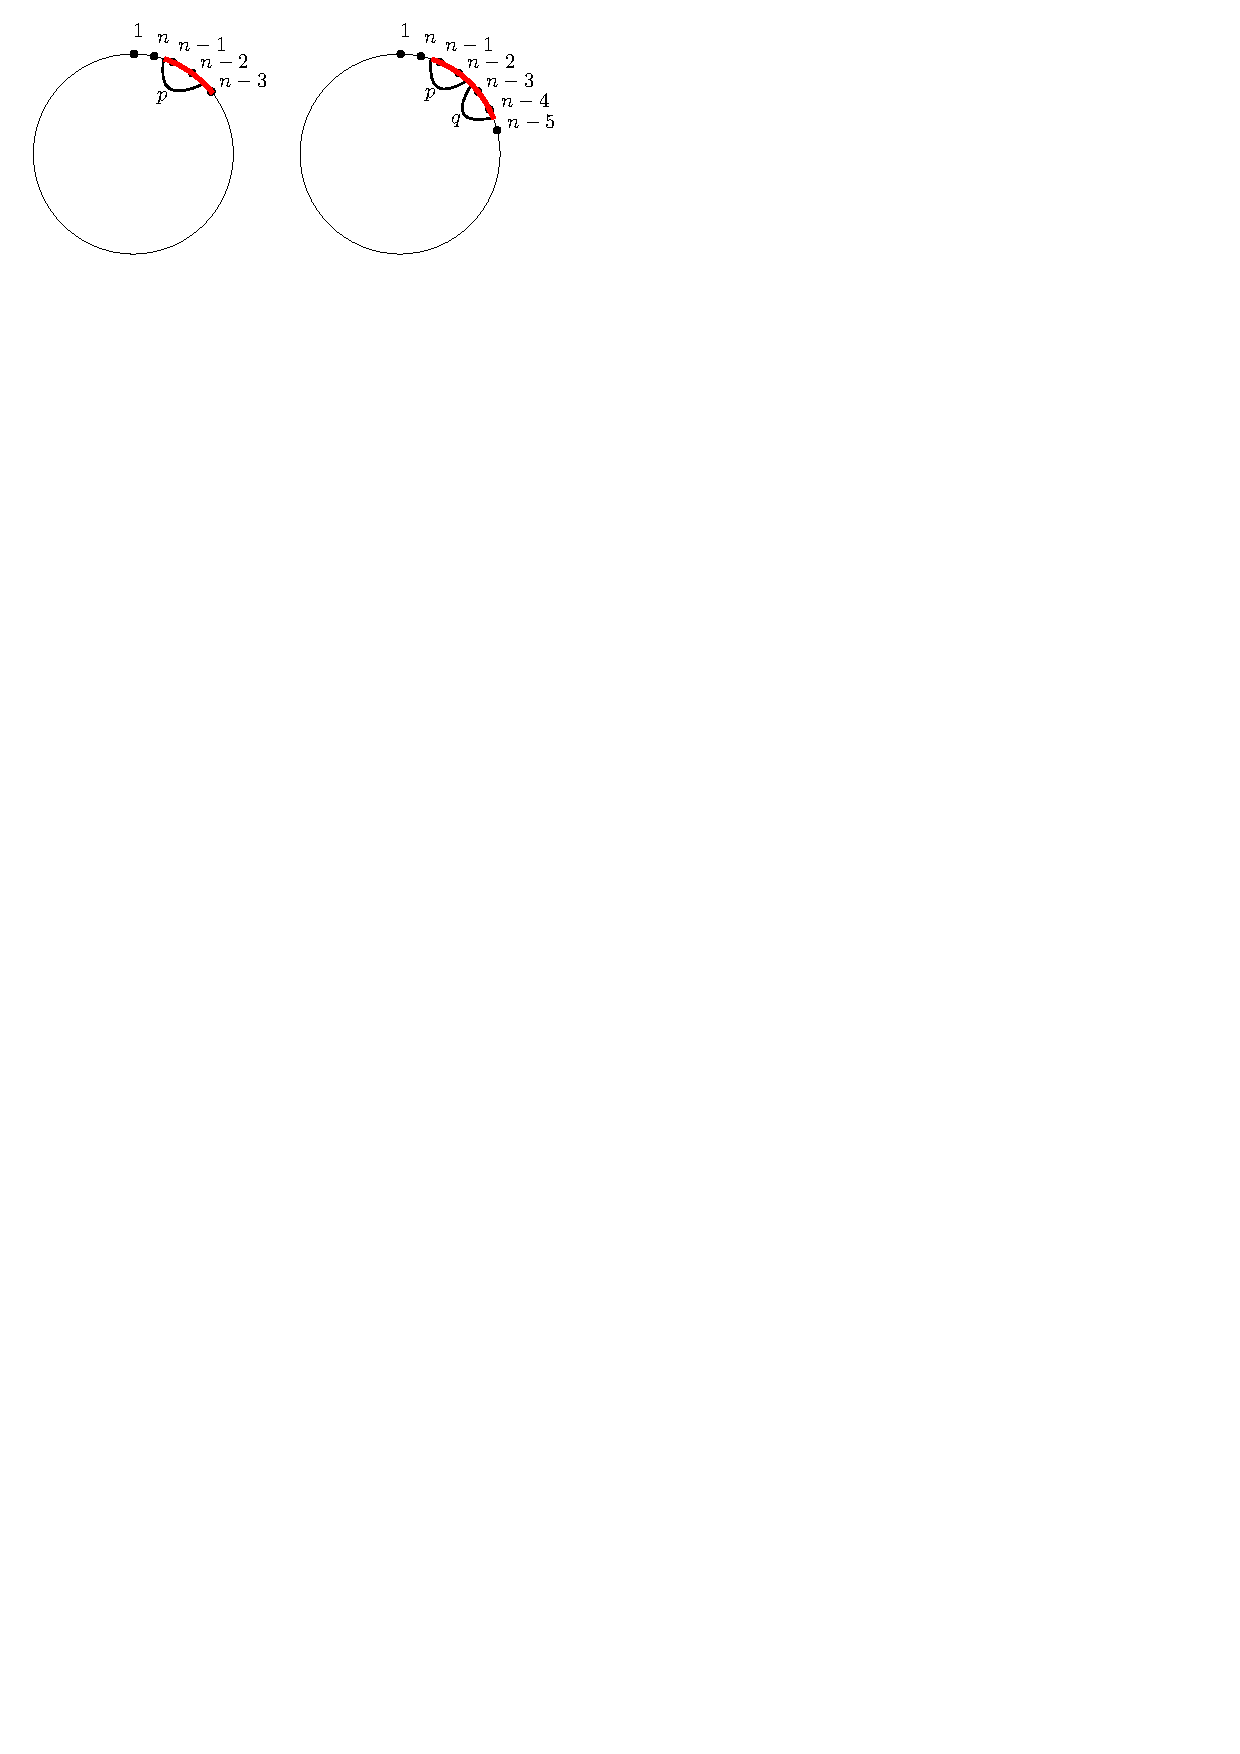
\includegraphics{specialp}
  \caption{The two cases for $W$ and $p$.  No other propagators can end in the fat red sections.  Other segments may have additional propagators ending in them.}\label{fig special p}
\end{figure}

\begin{proof}

The two possible cases for $W$ are illustrated in Figure~\ref{fig special p}; all references to the ``left hand case'' or ``right hand case'' below refer to the diagrams in this figure.

We first consider $I_1^{W}$, i.e. the set obtained by applying the Grassmann necklace algorithm to $W$ with starting vertex 1. Note that $n-3 \not\in I_1^{V}$: for the right hand case this is clear from the diagram (since Algorithm~\ref{alg:put GN on WLD} would assign $q$ no later than vertex $n-4$), while for the left hand case it follows from Lemma \ref{lem no fourth vertex}. Therefore when we start at vertex 1 and apply the Grassmann necklace algorithm to $W$, $p$ is the only remaining unassigned propagator when we reach vertex $n-3$, and so we have $ I_1^{W}(p) = n-3$ and $I_1^W = I_1^V\cup \{n-3\}$.


Next consider $I_n^{W}$. From the figure we see that in both cases we have $I_n^{W}(p) = n$. We are now at vertex 1, and the unassigned propagators are exactly those that appear in $V$. Therefore the algorithm continues as in $I_1^{V}$, i.e. we have $I_n^{W} = I_1^{V} \cup \{n\}$. By a similar argument, we must have $I_{n-1}^{W} = I_n^{V} \cup \{n-1\}$.

Now consider $I_{n-2}^{W}$. If $n-2\not\in I_{n-2}^{V}$ (i.e. $n-2$ supports no propagators in $V$), then in $W$ the algorithm assigns $p$ to $n-2$ and this does not affect the rest of the construction of $I_{n-2}^{V}$, so we obtain $I_{n-2}^{W} = I_{n-2}^{V}\cup \{n-2\}$ as above.

On the other hand, if $n-2\in I_{n-2}^{V}$ then we must be in the right hand case of Figure~\ref{fig special p} and the algorithm assigns $q$ to vertex $n-2$ in both $V$ and $W$ (since $q$ is always the clockwise-most propagator supported on vertex $n-2$; see Figure~\ref{fig special p}). If $n-1 \not\in I_{n-2}^{V}$, then in $W$ the algorithm assigns $p$ to $n-1$ and then proceeds identically to $I_{n-2}^{V}$ for the remainder of its steps; thus $I_{n-2}^{W} = I_{n-2}^{V}\cup \{n-1\}$ in this case.

Finally, if $n-2,n-1 \in I_{n-2}^{V}$ then in $W$ the algorithm assigns $q$ to $n-2$ and $p$ to $n-1$ as above, but this is different to what occured in $I_{n-2}^{V}$ so we cannot use the same argument as above. We are now at vertex $n$ and only propagators $p$ and $q$ have been assigned; thus we are proceeding as in the construction of $I_n^{V}$ but without propagator $q$. By Lemma~\ref{vertex cyclic int lem} we know that $q$ was assigned to $n-5$ by $I_n^{V}$, and from the diagram we see that the only way this could occur is if all other propagators in $V$ had already been assigned when we reached vertex $n-5$; thus $q$ was the final propagator to be assigned in $I_n^{V}$. Therefore $I_{n-2}^{W} = (I_{n}^{V} \setminus \{n-5\}) \cup \{n-1, n-2\}$ in this case. This completes all cases for $I_{n-2}^{W}$.

The arguments for $I_k^{W}$ ($1< k < n-2$) proceed analagously to those of $I_{n-2}^{W}$, with one simplification: we cannot have both $n-3$ and $n-2$ in $I_k^{V}$ since $q$ is the only propagator that could be assigned to either of them, and it cannot be assigned to both.

This covers all cases and hence completes the proof.
\end{proof}

\begin{figure}
  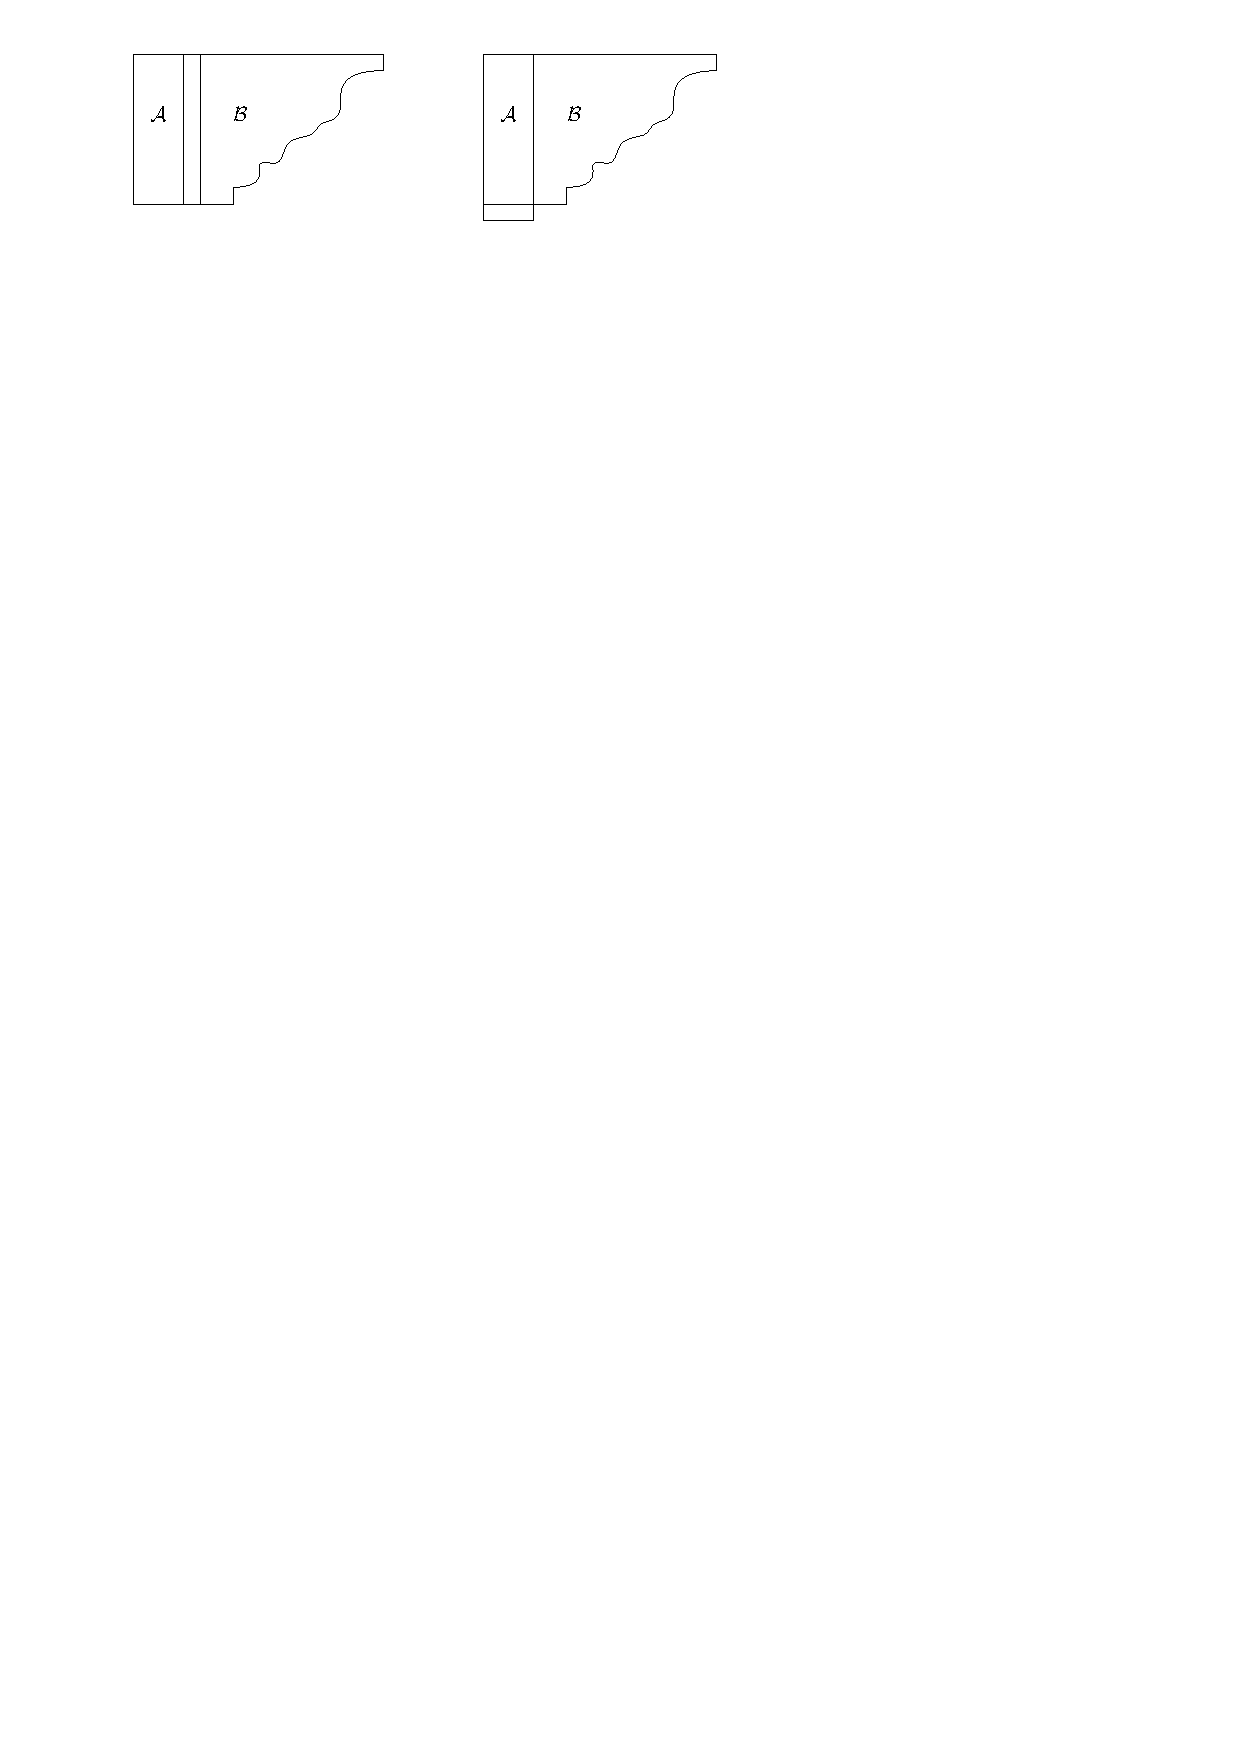
\includegraphics{Le_diagrams}
  \caption{Le diagrams for $V$ (left) and $W$ (right).}\label{fig Le}
\end{figure}

\note{When doing the final formatting, try to ensure that Figure \ref{fig Le} and Lemma \ref{lem shape} are on the same page}
\begin{lem}\label{lem shape}
  Let $V$ and $W$ be as in Lemma~\ref{lem I}.
  The shape of the Le diagram of $V$ can be built from left to right of the following blocks: a rectangle which is 3 columns wide, one more column of the same height, and a partition shape with at most as many rows as the rectangle.
  The shape of the Le diagram of $W$ can be built from left to right of the following blocks: a rectangle with 3 columns and one more row than the first rectangle of $V$, and the same partition shape as in $V$.
\end{lem}

\begin{proof}
See Figure~\ref{fig Le} for an illustration of the shapes described in the statement of the lemma.

Recall that $I_1$ determines the shape of the Le diagram. By Lemma~\ref{lem I} we know that
\newline ${n,n-1,n-2, n-3 \not\in I_1^{V}}$ (which yields the leftmost four columns of the diagram for $V$) and that $I_1^{W} = I_1^{V}\cup \{n-3\}$. This implies that the right hand boundary of the shape of $V$ is the same as the right hand boundary of the shape of $W$ except that $W$ has one additional row of 3 boxes while $V$ has an additional column in the $n-3$ position; that is, an extra column fourth from the left.
\end{proof}

As illustrated in Figure~\ref{fig Le}, the pieces of the Le diagrams of $V$ and $W$ will be called $\mathcal{A}$ and $\mathcal{B}$ in what follows. Over the course of the next few lemmas we will prove that the plusses in the $\mathcal{B}$ parts of each diagram are identical, and that the relationship between the plusses in the $\mathcal{A}$ regions can be described explicitly.


We do this by applying Algorithm~\ref{alg:GN to Le}, which constructs the Le diagram associated to a Grassmann necklace, to the Grassmann necklaces of $V$ and $W$. As described in Section [ref], if Algorithm~\ref{alg:GN to Le} places a $+$ in the box with row index $i$ and column index $j$, we say that this plus is in the $i \rightarrow j$ position, and refer to it as the plus defined by ``the (hook) path from $i$ to $j$''. Note that the collection of paths contributed by a single Grassmann necklace term  must be non-crossing.



Finally, we also note that when we speak of a plus in the Le diagram of $V$ being the same as in $W$ or vice versa, we mean that the position of the plus in $\mathcal{A}$ or $\mathcal{B}$ is the same; because of the column insertion the absolute indices may differ.




\begin{lem}\label{lem n and n-1}
Let $V$ and $W$ be as in Lemma~\ref{lem I}.
Then $I_n^{W}$ and $I_{n-1}^{W}$ together yield the same plusses as $I_n^{V}$ did, along with two extra plusses which appear in the leftmost two boxes of the bottom row of the Le diagram of $W$.
\end{lem}

\begin{proof}
By Lemma~\ref{lem I} we have $I_n^{W}= I_1^{V} \cup \{n\}$ and $I_1^{W} = I_1^{V} \cup \{n-3\}$. Thus 
\[I_1^{W} \setminus I_n^{W} = \{n-3\}, \qquad \qquad I_n^{W} \setminus I_1^{W} = \{n\},\]
and so by Algorithm~\ref{alg:GN to Le} we have a plus in the $(n-3) \rightarrow n$ position, i.e. in the leftmost box of the bottom row.

Also by Lemma~\ref{lem I} we have $I_{n-1}^{W} = I_n^{V} \cup \{n-1\}$. Recall from the proof of Lemma~\ref{lem I} that $n-3,n-2,n-1,n \not\in I_1^V$; therefore $I_1^W\setminus I_{n-1}^W = (I_1^V \setminus I_n^V) \cup\{n-3\}$, and $n-3$ is maximal in this set. Similarly, 
\[I_{n-1}^W \setminus I_1^W = (I_n^V \setminus I_1^V) \cup \{n-1\} \subseteq \{n-1,n\},\]
where the final inclusion follows from the definition of Grassmann necklace. In particular, $n-1$ is minimal in this set, so Algorithm~\ref{alg:GN to Le} yields a plus in the $(n-3) \rightarrow (n-1)$ position (i.e. the second box in the bottom row of the Le diagram of $W$) along with any plusses yielded by $I_n^V$.
\end{proof}

% Additionally $n-3\not\in I_{n}^{V}$ since if it were then $n-3$ would also be in $I_1^{V}$ and hence propagator $p$ could not contribute $n-3$ to $I_1^{W}$ in contradiction to Lemma~\ref{vertex cyclic int lem}.  Similarly $n-1, n-2\not\in I_n^{V}$.  Thus the paths putting the plusses in from $I_n^{V}$ lie completely in $\mathcal{B}$ or take some vertical boundary edge $>n-3$ to $n$.   Now view these paths in the Le diagram of $W$ and note that the path $n-3\rightarrow n-1$ is compatible, and so these paths together build the plusses that $I_{n-1}^{W}$ contributes.  That is, we get all the plusses from $I_{n}^{V}$ along with a $n-3\rightarrow n-1$ plus, that is a plus in the second to the right box of the bottom row.


\begin{lem}\label{lem n-2 good}
  Let $V$ and $W$ be as in Lemma~\ref{lem I}, and suppose that $n-2 \not\in I_{n-2}^{V}$. Then $I_{n-2}^{W}$ contributes all of the same plusses as $I_{n-1}^{V}=I_{n-2}^{V}$, along with a new $(n-3)\rightarrow (n-2)$ plus.
\end{lem}

\begin{proof}
If $n-2\not\in I_{n-2}^{V}$ then $I_{n-1}^{V}=I_{n-2}^{V}$ by definition, and by Lemma~\ref{lem I} we have $I_{n-2}^{W} = I_{n-1}^{V} \cup \{n-2\}$.  Note that $n-3\not\in I_{n-2}^{V}$ by Lemma~\ref{lem no fourth vertex}.  Therefore the paths controlling the plusses contributed by $I_{n-2}^{W}$ are exactly the paths for $I_{n-1}^{V}$ along with the $(n-3)\rightarrow (n-2)$ path.  This gives the statement of the lemma.
\end{proof}

\begin{lem}\label{lem n-2 bad}
Let $V$ and $W$ be as in Lemma~\ref{lem I}, and suppose that $n-2,n-1 \in I_{n-2}^{V}$.

Then $I_{n-2}^{W}$ and $I_{n-3}^{W}$ contribute the following plusses to the Le diagram of $W$
  \begin{itemize}
  \item An $(n-3)\rightarrow (n-2)$ plus and an $(n-5)\rightarrow (n-1)$ plus.
  \item All of the $I_{n-1}^{V}$ plusses.
  \item In the Le diagram of $V$, $I_{n-2}^{V}$ contributes an $n-5\rightarrow n-2$ plus and no other term in the Grassmann necklace of $V$ gives a plus in this column.  $I_{n-2}^W$ does not contribute this $+$ but yields an $n-5\rightarrow n-1$ plus instead.
  \item All other plusses of $I_{n-2}^{V}$.
  \item In the Le diagram of $V$, $I_{n-3}^{V}$ gives a plus in the $n-3$ column.  This $+$ is shifted over into the $n-2$ column in $W$.
  \item All other plusses of $I_{n-3}^{V}$.
  \end{itemize}
Furthermore, no element of the Gramann necklace of $V$ gives an $n-5\rightarrow n-1$ plus.
\end{lem}

\begin{proof}
  By Lemma~\ref{lem I} $I_{n-2}^{W}= (I_{n}^{V} - \{n-5\})\cup \{n-1,n-2\}$.  Also, by the location of $q$ in the WLD,  $n-2\not\in I_{n-3}^{V}$ and and $n-5$ is the index of the lowest vertical edge in $\mathcal{B}$.  Thus this section of the Gramann necklace of $V$ looks like
  \begin{equation}\label{eq necklace}
  I_{n-3}^{V} \underset{\substack{n-3\text{ out}\\n-2\text{ in}}}{\rightarrow} I_{n-2}^{V} \underset{\substack{n-2\text{ out}\\n-5\text{ in}}}{\rightarrow} I_{n-1}^{V} \underset{\substack{n-1\text{ out}\\\text{something in}}}{\rightarrow} I_{n}^{V} \underset{\substack{n \text{ out}\\\text{something in}}}{\rightarrow} I_1^{V}
  \end{equation}
  where the first ``something'' is either $n$ or an element of $I_1^{V}$ and the second ``something'' is an element of $I_1^{V}$.  Additionally all elements not explicitly mentioned must be in $I_1^{V}$ as they remain unchanged through this portion of the necklace.

  Using this information now determine the symmetric difference of $I_{n-2}^{V}$ and $I_1^{V}$: $n-1, n-2$ and possibly $n$ are in $I_{n-2}^{V}$ but not in $I_1^{V}$.  $n-5$ is in $I_1^{V}$ as are at least one and at most two other elements.  If there is one such element call it $a$.  If there are two call them $a$ and $b$ with $a>b$.  This means that the plusses in the Le diagram of $V$ coming from $I_{n-2}^{V}$ are as in the first part of Figure~\ref{fig messy}.  Stepping to $I_{n-1}^{V}$ simply removes the $n-5\rightarrow n-2$ path, see the second part of Figure~\ref{fig messy}.

  \begin{figure}
    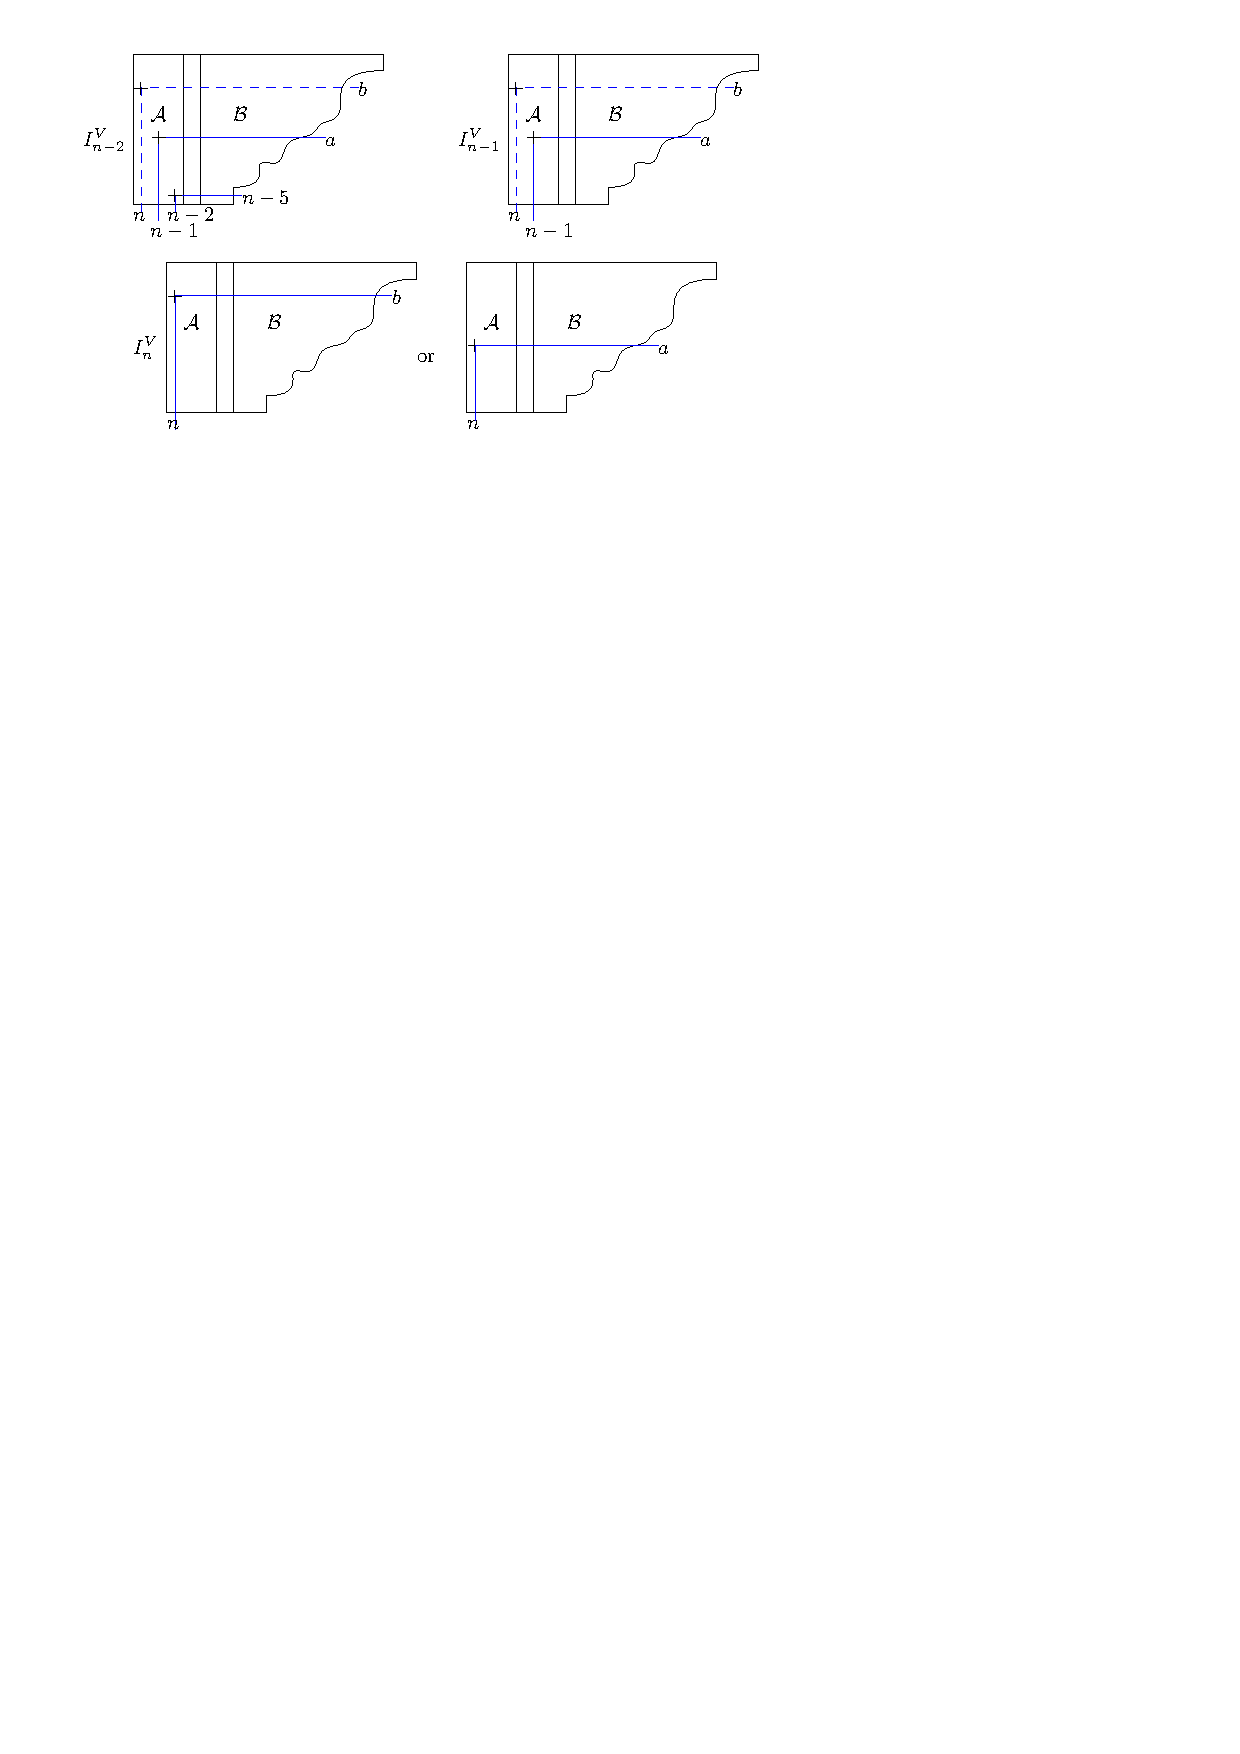
\includegraphics{messy}
    \caption{Plusses coming from $I_{n-2}^{V}$ (top left),  $I_{n-1}^{V}$ (top right) and $I_{n}^{V}$ bottom when $n-1, n-2\in I_{n-1}^{V}$.  The blue lines are the non-intersecting paths.  The dashed blue lines may or may not appear, but if one appears then they both do.}\label{fig messy}
  \end{figure}

  Stepping to $I_{n}^{V}$, $n-1$ is taken out and either $n$ is put in if it was not there before, or one of $a$ or $b$ is put in and hence no longer available as a right end for a path.  This gives two possible configurations illustrated in the bottom two parts of Figure~\ref{fig messy}.

  Now we know that $I_{n-2}^{W}  = (I_{n}^{V} - \{n-5\})\cup \{n-1,n-2\}$ so the paths for building plusses from $I_{n-2}^{W}$ go from the set $\{n-5, n-3\}$ along with whichever of $a$ and $b$ is not in $I_{n}^{V}$ to $\{n-2, n-1, n\}$.  This means that we get plusses as in Figure~\ref{fig messyD} where the left and right cases correspond to the left and right cases in the bottom parts of Figure~\ref{fig messy}

  \begin{figure}
     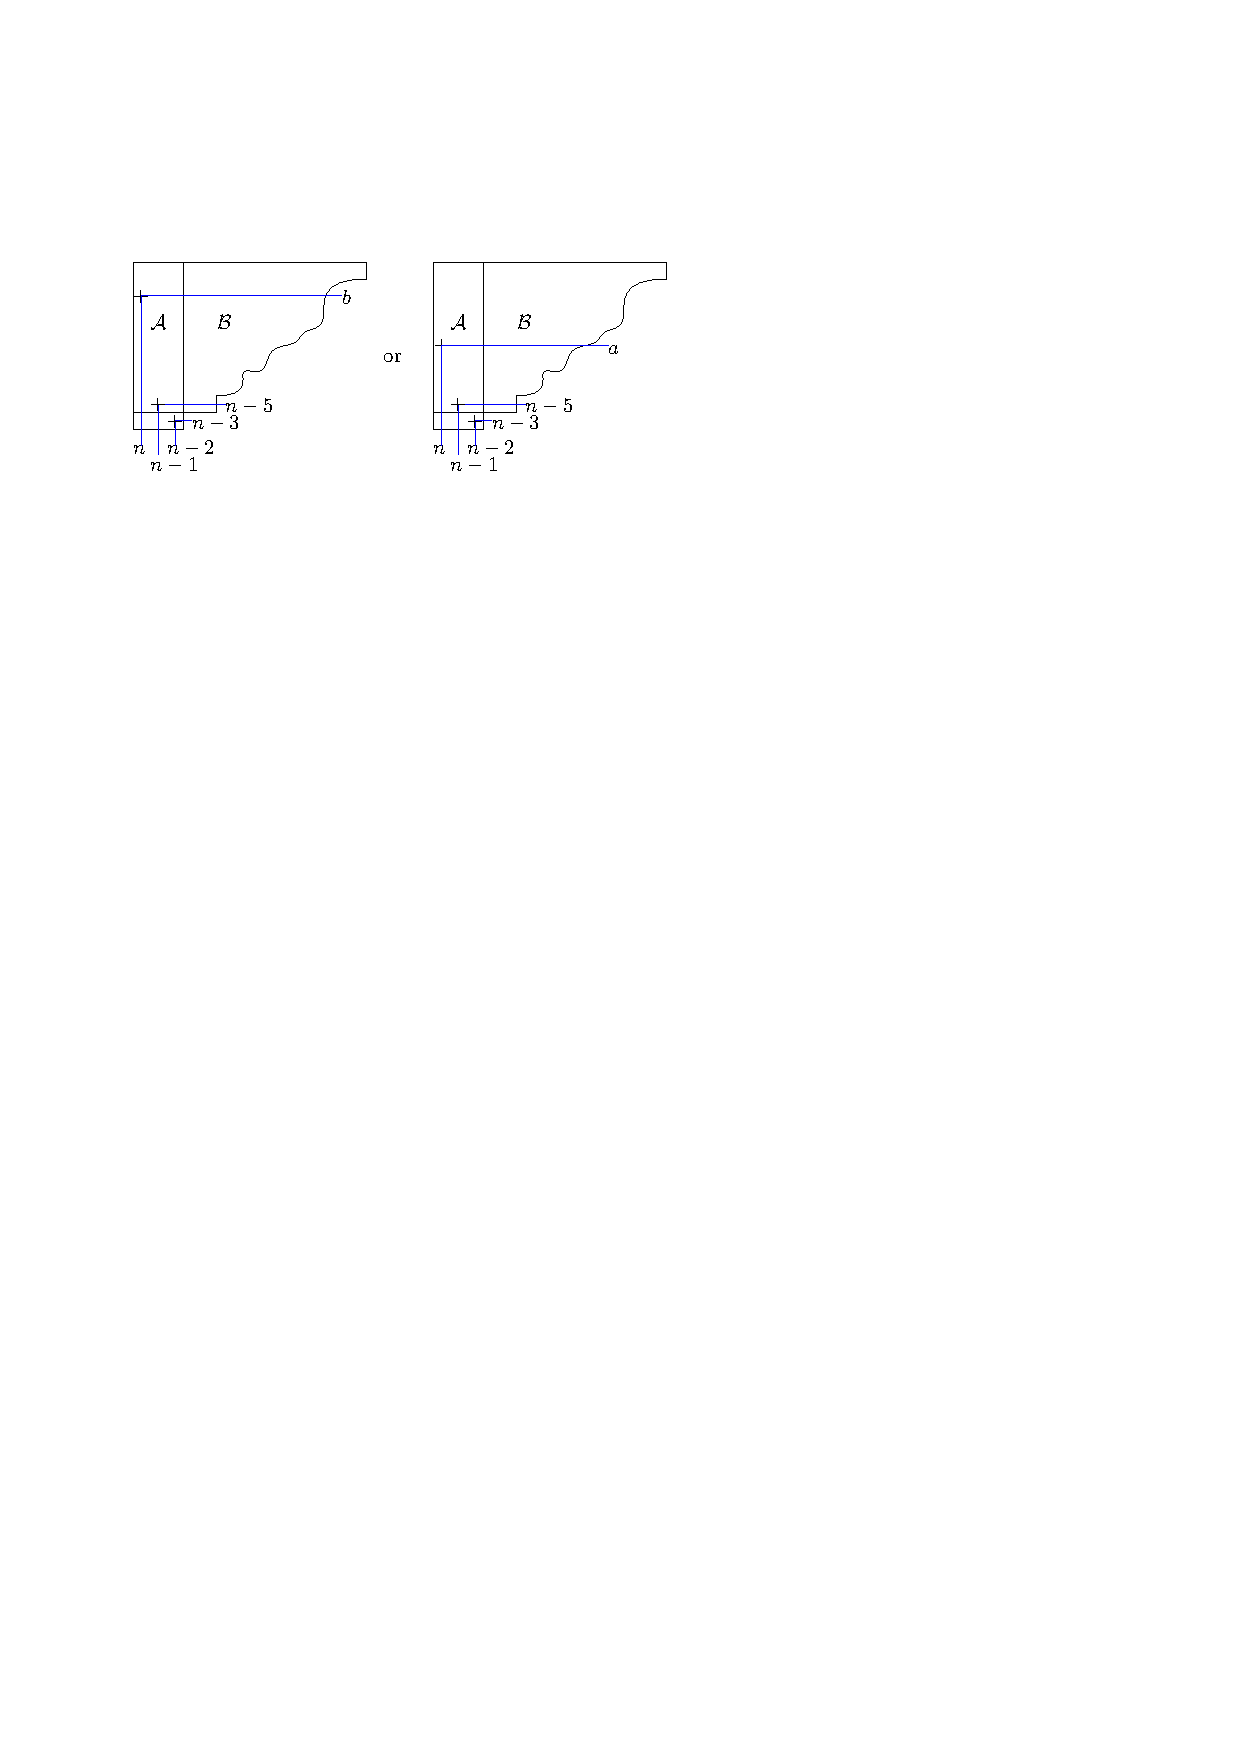
\includegraphics{messyD}
    \caption{Plusses coming from $I_{n-2}^{W}$.}\label{fig messyD}
  \end{figure}

  This proves the first item of statement of the lemma.

  Now consider $I_{n-3}^{V}$.  By \eqref{eq necklace} $I_{n-3}^{V}$ contributes the same plusses as $I_{n_2}^{V}$ except that it contributes an $n-5\rightarrow n-3$ plus in place of the $n-5\rightarrow n-2$ plus.  Also, we have $n-3\in I_{n-3}^{V}$ be the location of $q$ and so $I_{k}^{W} = I_k^{V}\cup\{n-2\}$.  Thus the paths for $I^{W}_{n-3}$ are the same as for $I^{V}_{n-3}$ except that the path that did go to $n-3$ now goes to $n-2$.  This cannot conflict with another path since \eqref{eq necklace} shows that $n-2$ only appears in $I_{n-2}^{V}$ among the necklace elements of $V$.

  Also note that $I_{n-3}^{V}, I_{n-2}^{V}$, and $I_{n-1}^{V}$ share their plusses outside of the $n-3$ and $n-2$ columns.  This proves the remaining statements of the lemma except the furthermore.

  Finally, suppose there were a $n-5\rightarrow n-1$ plus in the Le diagram of $V$.  By the algorithm, it would have to come when $n-5 \not\in I_j^{V}$.  By \eqref{eq necklace} this means that it would have to come from $I_{n-4}^{V}$, $I_{n-3}^{V}$, or $I_{n-2}^{V}$. The analysis above shows it does not come from $I_{n-3}^{V}$ or $I_{n-2}^{V}$.   Now, $n-4\in I_{n-4}^{V}$ by the location of $q$ and so $I_{n-4}^{V}$ must give an $n-5\rightarrow n-4$ plus and so cannot give an $n-5\rightarrow n-1$ plus.

\end{proof}



\note{This is a reorganised version of the previous lemma, keeping both in place for now for comparison.}
\begin{lem}\label{lem n-2 bad v2}
Let $V$ and $W$ be as in Lemma~\ref{lem I}, and suppose that $n-2,n-1 \in I_{n-2}^{V}$. Then:
  \begin{enumerate}
  \item $I_{n-2}^W$ contributes an $(n-3)\rightarrow (n-2)$ plus and an $(n-5)\rightarrow (n-1)$ plus, along with any plusses contributed by $I_n^V$.
  \item $I_{n-3}^W$ contributes the same plusses as $I_{n-3}^V$, except that the plus in the $n-3$ column is shifted one square left into the $n-2$ column.
  \item In the Le diagram of $V$, $I_{n-2}^{V}$ contributes an $(n-5)\rightarrow (n-2)$ plus and no other term in the Grassmann necklace of $V$ gives a plus in this column.  $I_{n-2}^W$ does not contribute this $+$ but yields the $(n-5)\rightarrow (n-1)$ plus from point (1) instead.
  \item All other plusses from $I_{n-2}^{V}$ and all plusses from $I_{n-1}^V$ were already contributed by $I_{n-3}^V$, so they yield no new information.
  \item No element of the Grassmann necklace of $V$ contributes a $(n-5)\rightarrow (n-1)$ plus.
  \end{enumerate} 
\end{lem}

\begin{proof}
  By Lemma~\ref{lem I} we have $I_{n-2}^{W}= (I_{n}^{V} \setminus \{n-5\})\cup \{n-1,n-2\}$ and $I_1^W = I_1^V\cup \{n-3\}$. We are necessarily in the case where $W$ admits a propagator $q$ (the right hand case of Figure~\ref{fig special p}) and we can see from the location of $q$ that $n-2\not\in I_{n-3}^{V}$ and that $n-5$ is the index of the lowest vertical edge in $\mathcal{B}$.  Thus this section of the Gramann necklace of $V$ looks like

  \begin{equation}\label{eq necklace}
  I_{n-3}^{V} \xrightarrow[\substack{n-3\text{ out}\\n-2\text{ in}}]{} I_{n-2}^{V} \xrightarrow[\substack{n-2\text{ out}\\n-5\text{ in}}]{} I_{n-1}^{V} \xrightarrow[\substack{n-1\text{ out}\\\text{something in}}]{} I_{n}^{V}  \xrightarrow[\substack{n \text{ out}\\\text{something in}}]{\text{\ no change, {\em or}\ }} I_1^{V}
  \end{equation}
  where the first ``something'' is either $n$ or an element of $I_1^{V}$, and the second ``something'' (if it exists) is an element of $I_1^{V}$. If $n\not\in I_n^V$ then $I_n^V = I_1^V$.

  Using this information we can determine the symmetric difference of $I_{n-2}^{V}$ and $I_1^{V}$, which has size $\leq 3$ by the definition of a Grassmann necklace. We have $n-1, n-2 \in I_{n-2}^{V} \setminus I_1^V$ for certain, and the third element (if it exists) must be $n$. On the other hand we have $n-5 \in I_1^{V} \setminus I_{n-2}^V$, along with at least one and at most two other elements.  If there is one such element call it $a$.  If there are two call them $a$ and $b$ with $a>b$.  

  This means that the plusses in the Le diagram of $V$ coming from $I_{n-2}^{V}$ are as in the first part of Figure~\ref{fig messy}.  Stepping to $I_{n-1}^{V}$ simply removes the $(n-5)\rightarrow (n-2)$ path (second part of Figure~\ref{fig messy}), so $I_{n-1}^V$ contributes no new information about the Le diagram of $V$.

  \begin{figure}
    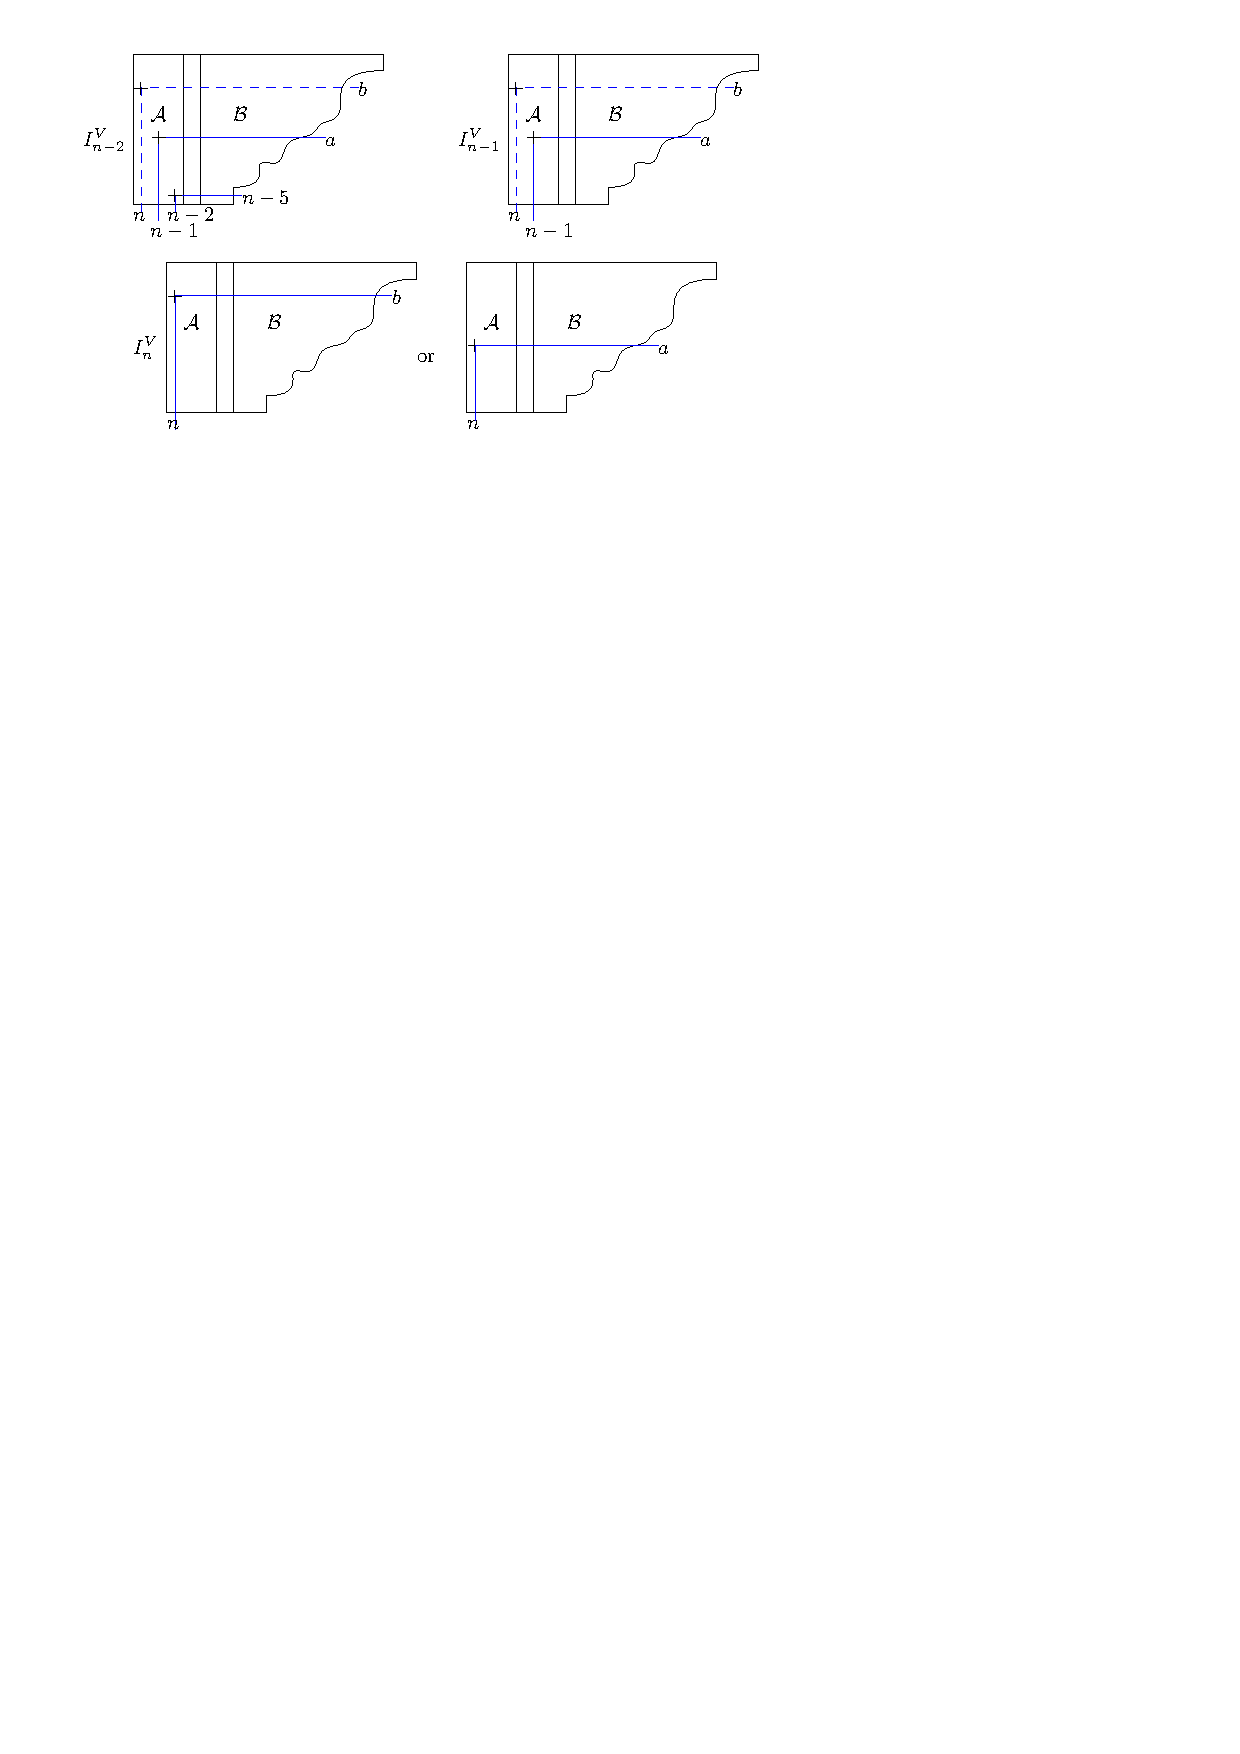
\includegraphics{messy}
    \caption{Plusses coming from $I_{n-2}^{V}$ (left) and  $I_{n-1}^{V}$ (right), in the case where $n-1, n-2\in I_{n-2}^{V}$.  The blue lines are the non-intersecting paths defining the position of the plusses.  The dashed blue lines may or may not appear, but if one appears then they both do.}\label{fig messy}
  \end{figure}

  \note{Remove the $I_n^V$ diagrams}

  %Stepping to $I_{n}^{V}$, $n-1$ is removed and either $n$ is put in if it was not there before, or one of $a$ or $b$ is put in and hence is no longer available as the starting point for a path.  This gives two possible configurations illustrated in the bottom two parts of Figure~\ref{fig messy}.

  With this information in hand, we can now tackle the points in the statement of the lemma. We know that 
  \[I_{n-2}^{W}  = (I_{n}^{V} - \{n-5\})\cup \{n-1,n-2\}, \quad n-5 \in I_1^W, \quad n-3\not\in I_{n-2}^W,\]
 and so the paths for building plusses from $I_{n-2}^{W}$ start at
 \[I_1^W \setminus I_{n-2}^W = \{n-3,n-5\} \cup (I_1^V \setminus I_n^V)\]
 and end at
 \[I_{n-2}^W \setminus I_1^W = \{n-2,n-1\}\cup(I_n^V \setminus I_1^V).\]
This means that $I_{n-2}^W$ contributes plusses as in Figure~\ref{fig messyD}, which proves point (1) and most of point (3). From equation \eqref{eq necklace} we see that $n-2$ appears only in $I_{n-2}^V$, so no other Grassmann necklace term for $V$ can contribute a plus in the $n-2$ column; this completes the proof of item (3).

  \begin{figure}
     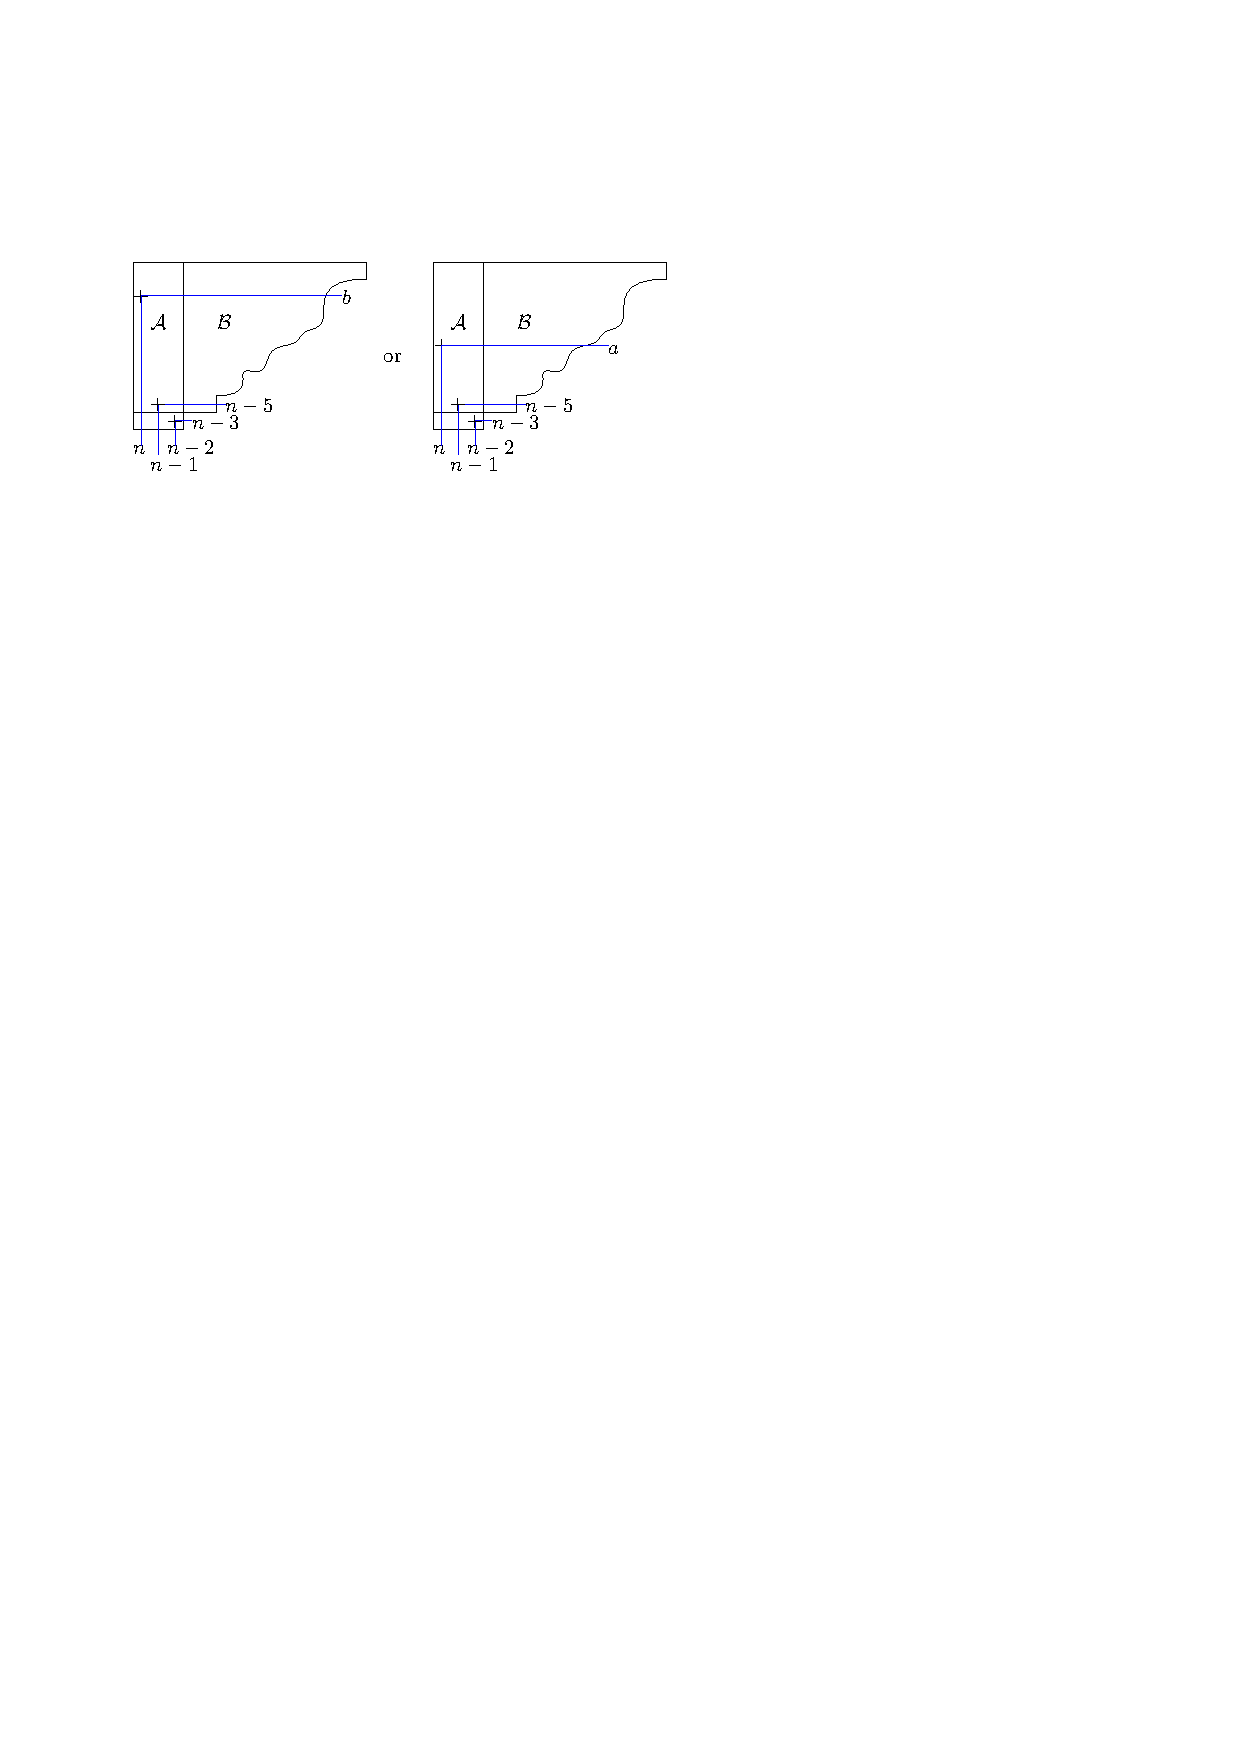
\includegraphics{messyD}
    \caption{Plusses coming from $I_{n-2}^{W}$.}\label{fig messyD}
  \end{figure}

\note{Modify this figure to include the case where there's no plus for column $n$.}

Now consider $I_{n-3}^{V}$.  By \eqref{eq necklace} $I_{n-3}^{V}$ contributes almost the same plusses as $I_{n-2}^{V}$: the only difference is that it contributes an $(n-5)\rightarrow (n-3)$ plus in place of the $(n-5)\rightarrow (n-2)$ plus.  Since we must have $n-3\in I_{n-3}^{V}$ (because the propagator $q$ exists in $V$), it follows from Lemma~\ref{lem I} that $I_{n-3}^{W} = I_{n-3}^{V}\cup\{n-2\}$.  Thus the paths for $I^{W}_{n-3}$ are the same as those for $I^{V}_{n-3}$ except that the path that did go to $n-3$ now goes to $n-2$.  This cannot conflict with another path since \eqref{eq necklace} shows that $n-2$ only appears in $I_{n-2}^{V}$ among the necklace elements of $V$.

This proves point (2), and combined with the observation above that $I_{n-1}^V$ contributes no new plusses compared to $I_{n-2}^V$, we also obtain item (4).


  Finally, if the Le diagram of $V$ did admit a $(n-5)\rightarrow (n-1)$ plus, it could only have been contributed by a necklace term that doesn't contain $n-5$.  By equation \eqref{eq necklace} the only terms that could have this property are $I_{n-2}^{V}$, $I_{n-3}^{V}$, and $I_{n-4}^{V}$, and the analysis above shows that $I_{n-2}^V$ and $I_{n-3}^V$ do not contribute a plus in this position.

  Recall that $n-5$ is the largest row index in the Le diagram of $V$, and $n-5 \in I_1^V \setminus I_{n-4}^V$ so $I_{n-4}^V$ does contribute a path starting at $n-5$. Since $n-4 \in I_{n-4}^V$ by the location of the propagator $q$, we must also have a path ending at $n-4$. Since the paths cannot cross, this implies that $I_{n-4}^V$ must contribute a $(n-5) \rightarrow (n-4)$ plus, and hence cannot contribute a $(n-5)\rightarrow (n-1)$ plus. This proves point (5) and completes the proof of the lemma.
\end{proof}



\begin{lem}\label{lem other k}
  Let $V$ and $W$ be as in Lemma~\ref{lem I}, and suppose that if $n-2\in I_{n-2}^{V}$ then $n-1\in I_{n-2}^{V}$ also. Then for each $k$ in the range $1<k<n-2$, $I_k^{W}$ contributes the same plusses as $I_{k}^{V}$, except that if $I_{k}^{V}$ contributed a plus in the $n-3$ column of the Le diagram of $V$ then this plus is shifted one square left in the Le diagram of $W$, and no plus was already in that location in the Le diagram of $W$.
\end{lem}

\begin{proof}
Recall that $I_1^W = I_1^V\cup \{n-3\}$ and that $n-2,n-1,n \not\in I_1^W$.

  If $n-3\not\in I_{k}^{V}$ then by Lemma~\ref{lem I} we have $I_{k}^{W} = I_k^{V}\cup \{n-3\}$.  Then since $n-3$ is the largest element of $I_1^{W}$ this transformation leaves the disjoint paths unchanged and so the plusses carry over from $V$ to $W$ directly.

  If $n-3\in I_{k}^{V}$ then $I_k^V$ must contribute a plus in the $n-3$ column of the Le diagram of $V$, and by Lemma~\ref{lem I} we have $I_{k}^{W} = I_k^{V}\cup \{n-2\}$. If $n-2$ supports no propagators in $V$ then certainly no pluses appear in the $n-2$ column of the Le diagram of $V$. If $n-2$ supports at least one propagator in $V$ then $n-2 \in I_{n-2}^V$ and so by hypothesis $n-1 \in I_{n-2}^V$ as well. By Lemma~\ref{lem n-2 bad}, the only necklace element of $V$ containing $n-2$ is $I_{n-2}^{V}$ and the corresponding plus is not contributed to the Le diagram of $W$ by $I_{n-2}^{W}$.

  Since $n-3 \in I_k^V \setminus I_1^V$, we must have a path from some vertical edge $i$ to the bottom edge $n-3$ in the Le diagram of $V$.  In the Le diagram of $W$, the index $n-3$ labels a vertical edge with no path starting at it (since $n-3$ belongs to both $I_1^W$ and $I_k^W$), and there must be a path leading to $n-2$ since $n-2 \in I_k^W \setminus I_1^W$.  By the previous paragraph no other path from $I_k^V$ could end at $n-2$, and since the paths cannot cross we conclude that the $i\rightarrow (n-3)$ path in the Le diagram of $V$ must become a $i\rightarrow (n-2)$ path in the Le diagram of $W$. All other paths are unchanged.

   Thus the plus contributed by $I_k^V$ in the $n-3$ column of the Le diagram of $V$ is shifted into the $n-2$ column in the Le diagram for $W$, where there was no plus before, and no other plusses are changed.
\end{proof}

\begin{thm}
  The number of plusses in the Le diagram of an admissible Wilson loop diagram is three times the number of propagators.
\end{thm}

\begin{proof}
  The proof is by induction on the number of propagators.

  First note that a Wilson loop diagram $W$ with one propagator supported on vertices $i<j<k<\ell$ has Le diagram a single row with $|W|-i$ boxes.  Labelling the columns from left to right by $|W|, \ldots, |W|-i+1$, by the algorithm there are plusses in the $j$, $k$, and $\ell$ positions.

  Now consider Wilson loop diagrams with $k>1$ propagators.  By Lemma~\ref{lem uncovered} it suffices to prove the result for weakly admissible Wilson loop diagrams with $k$ propagators and no non-supporting vertices.  By Lemma~\ref{lem dihedral} it suffices to prove the result for at least one Wilson loop diagram from each dihedral orbit.  Take a weakly admissible Wilson loop diagram $W$ with $k$ propagators and no non-supporting vertices.  Make a dihedral transformation of $W$ if necessary so that $W$ has a propagator $p$ with the properties in Lemma~\ref{lem good p}.  

  We make one further simplification: if our $W$ is in Case 2 of Figure~\ref{fig special p} and $n-1$ supports only $p$ but $n-2$ supports at least one other propagator, then flip $W$ on the line perpendicular to the edge from $n-2$ to $n-1$ to obtain a diagram with the configuration of Case 1. This eliminates the possibility that we could have $n-2 \in I_{n-2}^W$ but $n-1 \not\in I_{n-2}^W$. 

  This diagram will be our $W$ for the remainder of the proof. Let $V$ be $W$ with $p$ removed. 

  From Lemma~\ref{lem shape} we know how the shapes of the Le diagrams of $V$ and $W$ are related; let $\mathcal{A}$ and $\mathcal{B}$ be as described after that lemma.  Lemmas~\ref{lem n and n-1}, \ref{lem n-2 good}, and \ref{lem n-2 bad} tell us that the three boxes of the bottom row of the Le diagram of $W$ each have a plus.  Lemmas~\ref{lem n and n-1} through \ref{lem other k} show that there is a bijection between the plusses of the Le diagram of $V$ and the plusses of the Le diagram of $W$ that are not in the bottom row.  This bijection can be described as follows:
  \begin{itemize}
  \item All plusses from $\mathcal{B}$ for $V$ maintain their positions in $\mathcal{B}$ for $W$.
  \item All plusses from the leftmost two columns (the $n$ and the $n-1$ columns) of $\mathcal{A}$ for $V$ maintain their positions in $\mathcal{A}$ for $W$.
  \item If there is a plus in the $n-2$ column of $\mathcal{A}$ in $V$ then Lemma~\ref{lem n-2 bad} applies, so there is exactly one such plus.  This plus is mapped to the $(n-5)\rightarrow (n-1)$ plus for $W$.
  \item All plusses in the $n-3$ column for $V$ are shifted one square to the left in $\mathcal{A}$ for $W$, i.e. into the $n-2$ column.
  \end{itemize}
  Note that this map is reversible and hence bijective. Indeed, the only possible ambiguity is at the $(n-5)\rightarrow (n-1)$ plus in $W$ (if it exists), which could have come from either of the first or third bullet points. However, if the third bullet point applies then by Lemma~\ref{lem n-2 bad} there is no $(n-5)\rightarrow (n-1)$ plus in $V$, i.e. the first bullet point does not apply. 



  % If the Le diagram for $V$ has a plus in the $n-2$ column then Lemma~\ref{lem n-2 bad} applies. By the final part of Lemma~\ref{lem n-2 bad} there is no $n-5\rightarrow n-1$ plus in the Le diagram of $V$, and so the $n-5\rightarrow n-1$ plus of $W$ can be uniquely mapped to the plus in the $n-2$ column of the Le diagram of $V$.  If the Le diagram for $V$ has no plus in the $n-2$ column, then leave the $n-5\rightarrow n-1$ plus where it is in moving back to $V$.  This reverses the map.

Therefore the Le diagram of $W$ contains $3(k-1)$ plusses in bijection with the plusses from the Le diagram of $V$ and 3 new plusses in the bottom row, yielding $3k$ in total. Applying induction completes the proof.
\end{proof}



\section{Poles of Wilson Loop Integrals}



The results of Section~\ref{sec GN algorithm} allow us to relate the position of propagators in a Wilson loop diagram $W$ to minors of $C(W)$, which we use in this section to understand the denominator of the integral $I(W)$ associated to a Wilson loop diagram (see Definition~\ref{def R(W)}). 

The main result of this section is Theorem~\ref{thm denom}, which expresses the denominator $R(W)$ in terms of the Grassmann necklace of $W$. This simplifies the computation of $R(W)$ and allows us to directly relate the poles of the integral to the combinatorics of the diagram.

We first give an algorithm which extracts the required minors from the Grassmann necklace. 


\begin{algorithm}\label{alg WLD to denom via GN}
Let $W = (\cP,n)$ be a Wilson loop diagram, and let $C(W)$ be the matrix of $W$ as defined in \eqref{C(W) dfn} (see Section~\ref{section background}).
\begin{itemize}
  \item For each $i \in [n]$, we construct a factor $r_i$ as follows:
    \begin{itemize}
      %\item Use Algorithm~\ref{alg:put GN on WLD} to obtain a bijection between the propagators and the $i-1$st Grassmann necklace element, $I_{i-1}$.  (By convention set $I_{-1}=I_n$.)  Write $I_{i-1}(p)$ for the vertex associated to propagator $p$ under this bijection.
      %\item Use Algorithm~\ref{alg:put GN on WLD} to obtain a bijection between the propagators and the $i$th Grassmann necklace element, $I_{i}$.  Write $I_{i}(p)$ for the vertex associated to propagator $p$ under this bijection.
      \item Let $S_i = \{p \in \cP \ | \ I_{i-1}(p) \neq I_i(p)\}$. (By convention, set $I_{-1} = I_n$.)
	  %\item Write $\Delta_{I_i}$ for the determinant of the $k \times k$ minor of $C(W)$ with columns indexed by $I_i$.
      \item Let $r_i$ be the determinant of the $|S_i|\times |S_i|$ minor of $C(W)$ with rows indexed by $S_i$ and columns indexed by $I_i(S_i)$.  %$\Delta_{I_i}$ with all variables from rows associated to $p\not\in S_i$ set to $1$.
    \end{itemize}
  \item Define $R = \prod_{i=1}^n r_i$.
\end{itemize}
\end{algorithm}

As we discuss the algorithm it will also be useful to have the notation $\Delta_{I_i}$ for the determinant of the $k\times k$ minor of $C(W)$ with columned indexed by $I_i$.

As we take each $r_i$ to simply be the determinant of a particular submatrix of $C(W)$, the sign of each $r_i$ is well-defined.  The goal is to show that $R$ is equal to the denominator of the Wilson loop diagram as defined in Definition~\ref{def R(W)}.
%  However, we will not be interested in these signs as they only contribute an overall sign to $R$ and our main theorem in this section (Theorem~\ref{thm denom}) will simply be to show that $R$ is equal up to a $\mathbb{Q}$-multiple to the denominator of the Wilson loop diagram (see Definition~\ref{def R(W)}). 

\begin{figure}
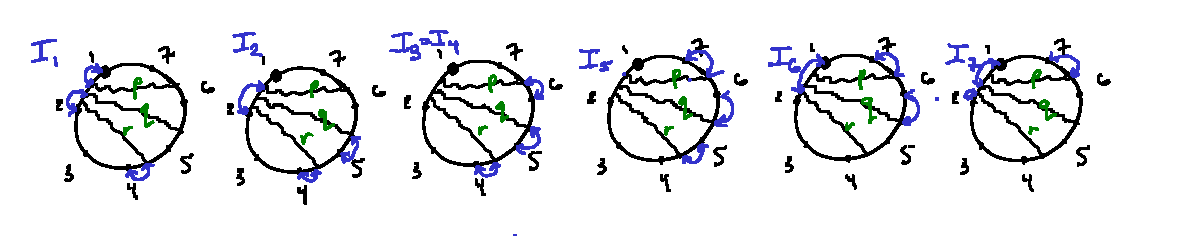
\includegraphics{egWLD_forR}
\caption{Example WLD for illustrating Algorithm~\ref{alg WLD to denom via GN} and bijections between propagators and vertices for each Grassmann necklace element.}\label{fig R eg}
\end{figure}

\begin{eg}
Consider the Wilson loop diagram in Figure~\ref{fig R eg}. Assigning propagators $p$, $q$, $s$ to rows $1,2,3$ respectively, we obtain the matrix
\[
C(W) = \begin{bmatrix} a & b & 0 & 0 & 0 & c & d \\ e & f & 0 & 0 & g & h & 0 \\ i & j & 0 & k & l & 0 & 0 \end{bmatrix}
\]
The Grassmann necklace of this diagram is 
\begin{gather*}I_1 = \{1,2,4\}, I_2 = \{2,4,5\}, I_3 = \{4,5,6\}, I_4=\{4,5,6\},\\ I_5=\{5,6,7\}, I_6 = \{6,7,1\}, I_7=\{7,1,2\}. \end{gather*}  
Figure~\ref{fig R eg} indicates the pairings between propagators and vertices for each $i \in [1,7]$.  

From $I_1$ to $I_2$, the propagators $p$ and $q$ change which vertex they are assigned to but $r$ is assigned to vertex 4 in both, so $S_2 = \{p,q\}$.  Then
\[
\Delta_{I_2}=\det\begin{bmatrix} b & 0 & 0 \\ f & 0 & g \\ j & k & l \end{bmatrix} = kgb, \qquad r_2 = \det\begin{bmatrix} b & 0 & 0 \\ f & 0 & g \\ 1 & 1 & 1 \end{bmatrix} = gb.
\]
where the 1s in the third row of the second matrix correspond to the fact that $I_1(s) = I_2(s)$.  Continuing likewise, we get $r_3 = c$, $r_4=1$ (since $I_4 = I_3$), $r_5 = lhd$, and $r_6 = i$.

At $I_7$ the situation is more complicated: we have $S_7 = \{q,s\}$, so we find that $\Delta_{I_7} = d(ej-fi)$ and $r_7 = ej-fi$. This quadratic factor corresponds to the fact that $q$ and $s$ share an edge {\em and} contribute both endpoints of that edge to $I_7$; see Proposition~\ref{prop alg gives rad} below.  

Finally, we have $r_1 = (af-be)k$.  Putting everything together, we obtain
\[
R = (af-be)kgbclhdi(ej-fi)
\]
which is squarefree and contains all factors of $\prod_{i=1}^{n}\Delta_{I_i}$. If one were to construct the denominator $R(W)$ associated to this Wilson loop diagram as per Definition~\ref{def R(W)}, we would find that we have $R(W) = R$.
\end{eg}


\begin{prop}\label{prop alg gives rad}
  With notation as in Algorithm~\ref{alg WLD to denom via GN} we have the following:
  \begin{enumerate}
    \item Each $\Delta_{I_i}$ is homogeneous, as is each $r_i$.
    \item Each $\Delta_{I_i}$ splits into linear and quadratic factors.  All linear factors of  $\Delta_{I_i}$ are single variables and all irreducible quadratic factors are $2\times 2$ determinants of single variables.
    \item Quadratic factors in $\Delta_{I_i}$ arise precisely when propagators $p$ and $q$ are supported on a common edge $(a,b)$ with $I_i(p)=a$ and $I_i(q)=b$.
    \item $r_i$ divides $\Delta_{I_i}$.
    \item The ideal generated by $R$ is the radical of the ideal generated by $\prod_{i=1}^{n}\Delta_{I_i}$.
  \end{enumerate}
\end{prop}

\begin{proof}
\begin{enumerate}
    \item The nonzero entries of $C(W)$ are independent indeterminates and so every $i\times i$ minor of $C(W)$ is either homogeneous of degree $i$ or is $0$.  Thus each $\Delta_{I_i}$ and each $r_i$ is homogeneous.  %Furthermore, each row contributes one factor to each term in the expansion of $\Delta_{I_i}$ so the result of setting the variables from a subset of rows to $1$ is still homogeneous.  Thus each $r_i$ is homogeneous.
    \item Using the expression for the determinant as a sum over permutations we see that $\Delta_{I_i}$ is a sum over bijections between $I_i$ and $\mathcal{P}$.  The nonzero terms in this sum are precisely those bijections such that each propagator is associated to one of its supporting vertices in $I_i$, since only those locations in $C(W)$ are nonzero.  Since the nonzero entries of $C(W)$ are independent there can be no cancellation between terms in this expansion.

Suppose $\Delta_{I_i}$ has an irreducible factor $f$.  Let $\mathcal{P}'$ be the set of propagators which contribute a variable to $f$ and let $J$ be the set of vertices which contribute a variable to $f$.

The first claim is that the minor of $C(W)$ associated to $\mathcal{P}'$ and $J$ is precisely $f$.

{\em Proof of claim}: By the structure of determinants we know that $\Delta_{I_i} = fg$, where $g$ involves only variables associated to propagators not in $\mathcal{P}'$ and associated to vertices not in $J$.  

Expanding out $fg$ yields a signed sum of monomials. In each of these monomials, $f$ contributes those variables associated both to a propagator in $\mathcal{P}'$ and to a vertex in $J$, and $g$ contributes those variables associated both to a propagator not in $\mathcal{P}'$ and to a vertex not in $J$, and no other variables appear.  


Since there is no cancellation between terms, this means that the full expansion over permutations of $\Delta_{I_i}$ contains no other nonzero terms and hence no other variables.  Therefore $\Delta_{I_i}$ is equal to the determinant of the matrix obtained by taking the submatrix of $C(W)$ with columns indexed by $I_i$ and setting any variables not appearing in $\Delta_{I_i}$ to $0$.  This new matrix is, up to permutations of rows and columns, a block matrix with one block for $\mathcal{P}'$ and $J$ and the other block for the complements.  Thus its determinant, and hence also $\Delta_{I_i}$, is the product of the minors for these two blocks.  By considering which variables appear, these two factors must also be $f$ and $g$, and so in particular $f$ is the minor of $C(W)$ associated to $\mathcal{P}'$ and $J$.  This proves the claim.

A consequence of this claim is that every linear factor of $\Delta_{I_i}$ is a $1\times 1$ minor of $C(W)$, hence is a single variable, and every irreducible quadratic factor of $\Delta_{I_i}$ is a $2\times 2$ minor of $C(W)$, hence is a $2\times 2$ determinant of single variables.

All that remains is to prove that $\Delta_{I_i}$ has no irreducible factors of degree 3 or more.  Suppose for a contradiction that $f$ is a factor of $\Delta_{I_i}$ of degree $\geq 3$. Note that by removing the propagators which come before those contributing to $f$ and changing $i$ to be the first vertex which contributes to $f$, we obtain a different admissible diagram for which $f$ still divides $\Delta_{I_i}$ but also $i\in I_i$ and
$i$ contributes to $f$.  Showing that this different admissible diagram gives a contradiction is sufficient, and so we may assume that $i\in I_i$ and $i$ contributes to $f$.  Finally, we can suppose that $W$ is minimal in number of propagators with the above occuring.

Let $p$ be the propagator such that $I_i(p) = i$. There are two cases to consider, depending on which edge $p$ is supported on.  These are illustrated in Figure~\ref{fig no big factors}

\begin{figure}
  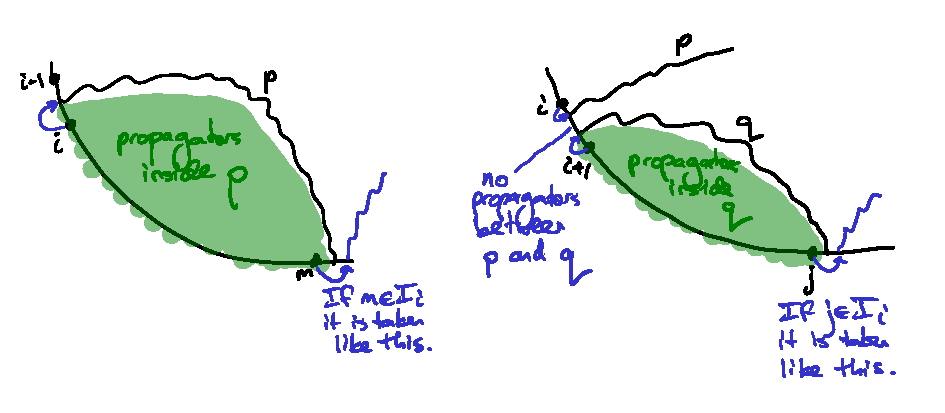
\includegraphics{no_big_factors}
  \caption{The two cases in the proof that no factors of $\Delta_{I_i}$ have degree 3 or more.}\label{fig no big factors}
\end{figure}

\textbf{Case 1}: Suppose $p$ has one end on the edge $(i-1, i)$.  Thus $p$ is supported on $(i-1, i, m, m+1)$ for some $m >_i i$, and $I_{i+1}(p) = m$ by Lemma~\ref{vertex cyclic int lem}.  

Let $S$ be the set of propagators inside $p$ along with $p$ itself. $I_i$ and $I_{i+1}$ can only differ once $p$ contributes to $I_{i+1}$, so $I_i(q) = I_{i+1}(q)$ for each $q \in S \backslash \{p\}$. Thus if a propagator contributes $m$ in $I_i$ then it must lie outside $p$.

If neither $m$ nor $m+1$ appear in $I_i$ then by Corollary~\ref{no coloops} $V(p) \cap I_i = \{i\}$, and so the row of $p$ in the matrix of $\Delta_{I_i}$ has only one nonzero entry; hence $\Delta_{I_i}$ has a linear factor contributed by $p$ and $i$, which is a contradiction.  So we must have at least one of $m$ and $m+1$ in $I_i$.  However, all propagators in $S$ are mapped by the function $I_{i}(\cdot)$ to vertices strictly before $m$, so the matrix giving $\Delta_{I_i}$ has the form
\[
\begin{bmatrix} A & B \\ 0 & C\end{bmatrix}
\]
where $A$ is the $|S|\times |S|$ matrix indexed by the propagators in $S$ and the vertices in $I_i(S)$. No other propagators can be supported on these vertices since all other propagators are outside of $p$, and $p$ is the first propagator supported at $i$; this explains the zero block.  Therefore $\Delta_{I_i} = \det A \det C$, and both factors are nontrivial since at least one of $m$ and $m+1$ appear in $I_i$.  If we remove the propagator outside of $p$ that contributes $m$ or $m+1$, we get a smaller diagram for which $\Delta_{I_i} = \det A$. This contradicts the minimality of our choices unless $\det A$ is quadratic, which in turn contradicts our assumption that $i$ and $p$ contribute to an irreducible factor $f$ of degree at least 3.

\textbf{Case 2}: Suppose $p$ has one end on the edge $(i, i+1)$.  If no other propagators are supported on $i$ then the column of $C(W)$ corresponding to vertex $i$ has only one nonzero entry in it, and so $\Delta_{I_i}$ has a linear factor contributed by $p$ and $i$; as above, this is a contradiction.  Thus we can take $q$ to be the propagator such that $I_i(q)=i+1$. We know that $q$ has one end on the edge $(i, i+1)$ and is adjacent to $p$ on that edge in the counterclockwise direction (see Figure \ref{fig no big factors}).  Write $(i, i+1, j, j+1)$ for the support of $q$.  The situation for $q$ is very similar to case 1: in particular, we have $I_{i+1}(q) = j$ by Lemma~\ref{vertex cyclic int lem} and so if $j\in I_i$ then the propagator which contributes $j$ is outside of $q$.  

Similarly to Case 1, let $S$ be the set of propagators inside $q$ along with $p$ and $q$ themselves. Then all propagators in $S$ are mapped by $I_i(\cdot)$ to vertices strictly before $j$ and no other propagators are supported on vertices strictly before $j$.  Thus the matrix giving $\Delta_{I_i}$ has the form
\[
\begin{bmatrix} A & B \\ 0 & C\end{bmatrix}
\]
where $A$ is the submatrix indexed by the propagators in $S$ and the vertices in $I_i(S)$. Again two things can now happen.  If some vertex $j$ or larger (with respect to $>_i$) belongs to $I_i$ then $B$ and $C$ are at least one column wide, and so the block form of the matrix gives a nontrivial factorization of $\Delta_{I_i}$.  This yields a contradiction as in Case 1: either $W$ contains unnecessary propagators which contradicts our minimality assumption, or $\det A$ is quadratic which contradicts the assumption that $p$ and $i$ contribute to $f$, an irreducible factor of degree at least 3.  

On the other hand, if no vertex $\geq_i j$ is in $I_i$ then $\Delta_{I_i} = \det A$.  Looking in more detail into $A$, note that the only vertices in the support of $p$ and $q$ which belong to $I_i$ are $i$ and $i+1$, and hence
\[
A = \begin{bmatrix} D & 0 \\ E & F\end{bmatrix}
\]
where $D$ is the $2\times 2$ matrix indexed by the propagators $p$ and $q$ and the vertices $i$ and $i+1$.  Thus $p$ and $i$ contribute to a quadratic factor of $\Delta_{I_i}$, once again contradicting our assumptions.

All cases have now been covered and so $\Delta_{I_i}$ has only irreducible factors of degree $2$ or less.

\item Suppose propagators $p$ and $q$ are supported on a common edge $(a,b)$, with $I_i(p)=a$ and $I_i(q)=b$.  Let $x_{p,a},x_{p,b},x_{q,a},x_{q,b}$ be the associated variables in $C(W)$. For any fixed bijection $\sigma$ from $\cP-\{p,q\}$ to $I_i -\{a,b\}$ for which each propagator is supported on its image under the bijection, we can extend $\sigma$ to a bijection of all propagators with $I_i$ in two ways: either $p\mapsto a$ and $q\mapsto b$ or $p\mapsto b$ and $q\mapsto a$.  The sum of the contributions of all these bijections to $\Delta_{I_i}$ is therefore the product of $x_{p,a}x_{q,b}-x_{p,b}x_{q,a}$ with the minor coming from $\cP-\{p, q\}$ and $I_i - \{a,b\}$.  Since there is no cancellation of terms in the expansion of $\Delta_{I_i}$, if any other terms appear then they will cause a factor which is not in the form described in the previous part.  Therefore no such terms exist and $x_{p,a}x_{q,b}-x_{p,b}x_{q,a}$ is a factor of $\Delta_{I_i}$.

Now let $f$ be a quadratic factor of $\Delta_{I_i}$.  By part (2) we know that $f$ is a $2\times 2$ minor coming from two propagators, call them $p$ and $q$, and two vertices, call them $a <_i b$.  It remains to show that $a$ and $b$ are adjacent.  From this we can conclude that $p$ and $q$ each have one end on $(a,b)$, as any other way for both $p$ and $q$ to be supported on two consecutive vertices would contradict noncrossing or the density requirement of admissibility.

As in the proof of part (2), make a new admissible diagram by removing the propagators which come before $f$ and set $i=a$.  The cases in the proof of part (2) show how $\Delta_{I_i}$ factors: in particular the vertices supporting the other end of $p$ either do not appear in $I_i$, or they contribute to a different factor of $\Delta_{I_i}$ than $p$ and $a$ do.  By assumption $b$ contributes to the same factor as $a$.  Therefore $(a,b)$ is an edge.

\item Consider $p\in S_i$, and note that $\Delta_{I_i}$ is homogeneous linear in the variables of the row corresponding to $p$.  By part (2), either exactly one variable in the row corresponding to $p$ appears in $\Delta_{I_i}$ and this variable is a factor of $\Delta_{I_i}$, or exactly two variables from the row corresponding to $p$ appear in $\Delta_{I_i}$ and they appear as part of a quadratic factor.  In the first case let the variable be $x$. Then $x$ is a factor of $\Delta_{I_i}$ and so in particular the monomial in $\Delta_{I_i}$ corresponding to the bijection between propagators and vertices of $I_i$ associates the column of $x$ to $p$.  Thus $x$ also appears in $r_i$ and since the matrix for $r_i$ is a minor of the matrix for $\Delta_{I_i}$ and every term in $\Delta_{I_i}$ involves $x$, we also have that every term in $r_i$ involves $x$ so $x$ is a factor of both $r_i$ and $\Delta_{I_i}$ and is the only variable from this row in either polynomial.  

Now suppose two variables from the row $p$ appear in a quadratic factor $f$.  By part (3), there is another propagator $q$ and an edge $(a,b)$ such that $f$ is the $2\times 2$ minor coming from $p, q$ and $a, b$, with $I_i(p)=a$, $I_i(q)=b$.  There are two situations which can occur, both illustrated in Figure~\ref{fig quadratic}; we show that in both cases it follows that $q \in S_i$ as well.

\begin{figure}
  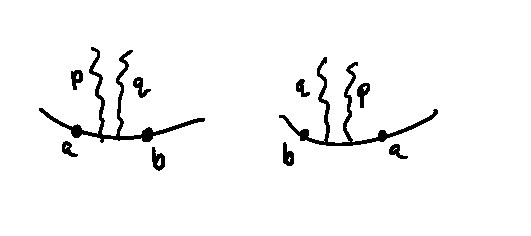
\includegraphics{quadratic}
  \caption{The situations giving a quadratic factor with variables appearing in $r_i$.}\label{fig quadratic}
\end{figure}

In both cases, since $I_{i-1}(p)\neq a$ by assumption it follows from Lemma~\ref{vertex cyclic int lem} that $I_{i-1}(p) <_{i-1} a$ and no other vertex supporting $p$ lies between $I_{i-1}(p)$ and $a$. In the case that $b<_i a$ and $q$ is taken before $p$ in $I_i$, this means that $I_{i-1}(p)=b$ and so $I_{i-1}(q)\neq b$.  Thus $q\in S_i$ and so $f$ is a factor of $r_i$.

Now consider the case where $a<_i b$, and suppose for contradiction that $q \not\in S_i$, i.e. that $I_{i-1}(q) = b$. Since $I_{i-1}(p) \neq a$, there must be some other propagator $s$ with $I_{i-1}(s) = a$ (else $I_{i-1}$ assigns $q$ to $a$). This propagator cannot lie on edge $(a,b)$ since by Lemma~\ref{vertex cyclic int lem} we must have $I_i(s) = a$ or $b$, contradicting the fact that $I_i(p) = a$ and $I_i(q) = b$; thus $s$ has an end on $(a-1,a)$ and is inside $p$ from the point of view of $i-1$.

Say $s$ is supported on $(j, j+1, a-1, a)$ and $p$ is supported on $(k, k+1, a, b)$ with $i-1 \leq_{i-1} k+1 \leq_{i-1} j+1$. But by Lemma~\ref{lem no fourth vertex}, if $I_{i-1}(s) = a$ then $a$ cannot be maximal in the support of $s$ with respect to $<_{i-1}$; thus we must have $i-1 = j+1$, and we are in the situation in figure~\ref{fig part 4}.

\begin{figure}
  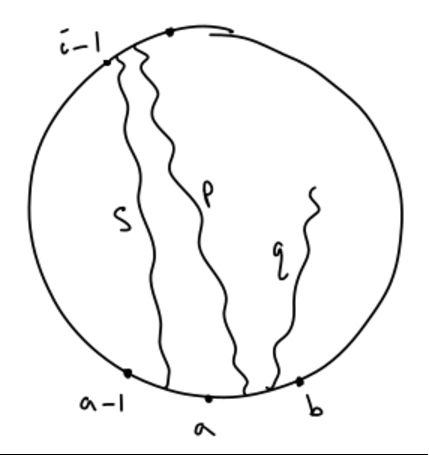
\includegraphics[scale=0.5]{part4}
  \caption{In order to obtain $I_{i-1}(s) = a$, propagators $s$ and $p$ must each have an end on the edge $(i-2,i-1)$.}\label{fig part 4}
\end{figure}

Since $p$ changed its association from $I_{i-1}$ to $I_i$, we have $I_{i-1}(p) = i-1$ by Lemma~\ref{vertex cyclic int lem}. From figure~\ref{fig part 4} it follows that $I_{i-1}$ assigns $p$ to $i-1$ and then proceeds identically to $I_i$ for all vertices inside $p$, implying that $I_{i-1}(s) = I_i(s)$. Since $I_{i-1}(s) = a$ and $I_i(s) \neq a$, this is a contradiction. 

Thus $q\in S_i$ after all, and so $f$ is a factor of $r_i$ as required.

  

% Thus $s$ is supported on $a$ but does not have an edge on $(a,b)$ and so $s$ must have an end on $(a-1, a)$ and so be inside $p$ from the point of view of $i-1$.  Say $s$ is supported on $(j, j+1, a-1, a)$ and $p$ is supported on $(k, k+1, a, b)$ with $i-1 \leq_{i-1} k+1 \leq_{i-1} j+1$.  Again by Lemma~\ref{lem susama}, immediately after $s$ contributes $a$ it must contribute $j$ and so $I_i(s)=j$.

% Finally we want to show $I_i(s)=j$ gives a contradiction.  If $k=j$ then $I_{i}(s)= k$, but $p$ has not yet been taken as $I_i(p)=a$ and $p$ comes before $s$ around $k$, so this is a contradiction.  If $k+1=j$ then similarly $I_{i}(s)=k+1$ and yet $p$ comes before $s$ around $k$, a contradiction to $I_i(p)=a$.  Now suppose $k+1 <_{i-1} j$ then we have $i-1 \leq_{i-1} k+1 <_{i-1} I_i(s) = j$ so $i\leq_{i} I_i(s)$ which gives that
% \[
% I_i(s) <_i I_{i-1}(s) \qquad \text{and} \qquad I_i(s) <_{i-1} I_{i-1}(s)
% \]
% \note{Is this known to be impossible by the proof sketch of Lemma~\ref{lem susama} that you emailed or something similar.  I'm thinking this proof is already too long and the fact that this is impossible would be better as a lemma.}

\item If $W$ has zero propagators then all $I_i=\emptyset$ and both $R$ and $\prod_{i=1}^n \Delta_{I_i}$ are equal to $1$, so the result holds in this case.  Now assume $W$ has at least one propagator.

First we show that every factor of $\prod_{i=1}^n \Delta_{I_i}$ divides $R$.  Take an irreducible factor $f$ of $\prod_{i=1}^n \Delta_{I_i}$. There exists some $i$ such that $f|\Delta_{I_i}$ but $f\!\!\nmid\!\! \Delta_{I_{i-1}}$, since otherwise the variables corresponding to the propagators contributing to $f$ which do not themselves appear in $f$ could never appear, contradicting Lemma~\ref{vertex cyclic int lem}.  If $f$ is a linear factor, say from associating propagator $p$ to vertex $a$, then $I_{i}(p)=a$ and $I_{i-1}(p)\neq a$ so this factor appears in $r_i$.  If $f$ is a quadratic factor, say from associating propagators $p$ and $q$ to vertices $a$ and $b$ respectively, then again we cannot have both $I_{i-1}(p) = a$ and $I_{i-1}(q) = b$, else $f$ divides $\Delta_{i-1}$. However, by the proof of part (4), if one of $p,q$ belongs to $S_i$ then the other does as well.  Thus $f$ divides $r_i$.

Next we need to show that $R$ is squarefree.  Suppose $f^2|R$.  If $f$ is a linear factor, say from associating propagator $p$ to vertex $a$, then there must be two distinct points in the Grassmann necklace algorithm where $p$ changes from not being associated to vertex $a$ to being associated to vertex $a$.  This contradicts Lemma~\ref{vertex cyclic int lem}.  Now suppose $f$ is a quadratic factor, say from propagators $p$ and $q$ supported on the edge $(a, b)$ with $p$ before $q$ on the edge.  In this case it is not possible for any $I_i$ to associate $p$ to $b$ and $q$ to $a$.  Furthermore, we know by part (4) that $p$ changes from not being associated to $a$ to being associated to $a$ if and only if $q$ changes from not being associated to $b$ to being associated to $b$.  Thus $f^2|R$ implies that twice in the Grassmann necklace $p$ must change from not being associated to vertex $a$ to being associated to vertex $a$. This is again a contradiction, and so $R$ is squarefree.

Taking everything together we have that $R|\prod_{i=1}^n \Delta_{I_i}$, $R$ contains all factors of $\prod_{i=1}^n \Delta_{I_i}$ and $R$ is squarefree.  Therefore the ideal generated by $R$ is the radical of the ideal generated by $\prod_{i=1}^n \Delta_{I_i}$.
  \end{enumerate}
\end{proof}


\begin{thm}\label{thm denom}
  Given any admissible Wilson loop diagram $W$, let $\{I_1, \ldots I_n\}$ be the associated Grasmann necklace. Then the denominator of the integral, $R(W)$ (see Definition~\ref{def R(W)}), is the $R$ of Algorithm~\ref{alg WLD to denom via GN}, which is also, up to scalar multiple, the radical of $\prod_{i=1}^n \Delta_{I_i}$, where $\Delta_{I_i}$ is the determinant of the $k \times k$ minor indicated by $I_i$.  
\end{thm}

\note{Note that there is still a mention of scalar multiple in this theorem because it seems to me that the def of radical is only up to scalar multiple, but the part relating $R(W)$ to $R$ is exact with no scalar multiples.}

\begin{proof}
The equivalence up to scalar multiple of $R$ and the radical of $\prod_{i=1}^n \Delta_{I_i}$ is due to Proposition~\ref{prop alg gives rad}.  It remains to prove that $R(W)$ is the $R$ of Algorithm~\ref{alg WLD to denom via GN}.

To this end, first note that $R(W)$ and $R$ both have total degree $4|\mathcal{P}|$; the degree of $R(W)$ is immediate from the definition while that of $R$ follows from Lemma~\ref{vertex cyclic int lem}.  By Proposition~\ref{prop alg gives rad} every factor of $R$ is either a single variable or a quadratic factor coming from two propagators supported on a common edge.  The factors of each $R_e$ making up $R(W)$ in the notation of Definition~\ref{def R(W)} are all of this form and hence every factor of $R$ divides $R(W)$.
Finally, since $R$ is squarefree, this implies that $R(W)$ is a scalar multiple of $R$.

Finally then we need to check the scalar.  By Definition~\ref{def R(W)} each linear factor appears with coefficient $1$ and each $2\times 2$ deteriminant factor appears with the same sign as the determinant of the corresponding minor in $C(W)$.  Therefore $R=R(W)$.
\end{proof}


***explain why this result was interesting***



\begin{thebibliography}{10}

\bibitem{wilsonloop}
S. Agarwala, E. M. Amat.
\newblock Wilson loop diagrams and positroids.
\newblock {\em Commun. Math. Phys.} 2016.

\bibitem{reversingOh}
S. Agarwala, S. Fryer.
\newblock An algorithm to construct the Le diagram associated to a Grassmann necklace
\newblock \url{arXiv:1803.01726}

\bibitem{Gale}
D. Gale.
\newblock Optimal assignments in an ordered set: {A}n application of matroid theory.
\newblock {\em J. Combinatorial Theory}, 4: 176 - 180 (1968).

\bibitem{Oh}
S. Oh.
\newblock Positroids and {S}chubert matroids.
\newblock {\em J. Combin. Theory Ser. A}, 118(8):2426--2435, (2011)


\bibitem{Postnikov}
A.~Postnikov.
\newblock Total positivity, {G}rassmannians, and networks.
\newblock \url{arXiv:math/0609764}.


\end{thebibliography}


\end{document}
